\documentclass[]{book}
\usepackage{lmodern}
\usepackage{amssymb,amsmath}
\usepackage{ifxetex,ifluatex}
\usepackage{fixltx2e} % provides \textsubscript
\ifnum 0\ifxetex 1\fi\ifluatex 1\fi=0 % if pdftex
  \usepackage[T1]{fontenc}
  \usepackage[utf8]{inputenc}
\else % if luatex or xelatex
  \ifxetex
    \usepackage{mathspec}
  \else
    \usepackage{fontspec}
  \fi
  \defaultfontfeatures{Ligatures=TeX,Scale=MatchLowercase}
\fi
% use upquote if available, for straight quotes in verbatim environments
\IfFileExists{upquote.sty}{\usepackage{upquote}}{}
% use microtype if available
\IfFileExists{microtype.sty}{%
\usepackage{microtype}
\UseMicrotypeSet[protrusion]{basicmath} % disable protrusion for tt fonts
}{}
\usepackage[a4paper]{geometry}
\usepackage{hyperref}
\PassOptionsToPackage{usenames,dvipsnames}{color} % color is loaded by hyperref
\hypersetup{unicode=true,
            pdftitle={Intermediate distance sampling workshop - St Andrews 2017},
            pdfauthor={Laura Marshall, David L. Miller and Len Thomas},
            colorlinks=true,
            linkcolor=blue,
            citecolor=Blue,
            urlcolor=Blue,
            breaklinks=true}
\urlstyle{same}  % don't use monospace font for urls
\usepackage{color}
\usepackage{fancyvrb}
\newcommand{\VerbBar}{|}
\newcommand{\VERB}{\Verb[commandchars=\\\{\}]}
\DefineVerbatimEnvironment{Highlighting}{Verbatim}{commandchars=\\\{\}}
% Add ',fontsize=\small' for more characters per line
\usepackage{framed}
\definecolor{shadecolor}{RGB}{248,248,248}
\newenvironment{Shaded}{\begin{snugshade}}{\end{snugshade}}
\newcommand{\KeywordTok}[1]{\textcolor[rgb]{0.13,0.29,0.53}{\textbf{#1}}}
\newcommand{\DataTypeTok}[1]{\textcolor[rgb]{0.13,0.29,0.53}{#1}}
\newcommand{\DecValTok}[1]{\textcolor[rgb]{0.00,0.00,0.81}{#1}}
\newcommand{\BaseNTok}[1]{\textcolor[rgb]{0.00,0.00,0.81}{#1}}
\newcommand{\FloatTok}[1]{\textcolor[rgb]{0.00,0.00,0.81}{#1}}
\newcommand{\ConstantTok}[1]{\textcolor[rgb]{0.00,0.00,0.00}{#1}}
\newcommand{\CharTok}[1]{\textcolor[rgb]{0.31,0.60,0.02}{#1}}
\newcommand{\SpecialCharTok}[1]{\textcolor[rgb]{0.00,0.00,0.00}{#1}}
\newcommand{\StringTok}[1]{\textcolor[rgb]{0.31,0.60,0.02}{#1}}
\newcommand{\VerbatimStringTok}[1]{\textcolor[rgb]{0.31,0.60,0.02}{#1}}
\newcommand{\SpecialStringTok}[1]{\textcolor[rgb]{0.31,0.60,0.02}{#1}}
\newcommand{\ImportTok}[1]{#1}
\newcommand{\CommentTok}[1]{\textcolor[rgb]{0.56,0.35,0.01}{\textit{#1}}}
\newcommand{\DocumentationTok}[1]{\textcolor[rgb]{0.56,0.35,0.01}{\textbf{\textit{#1}}}}
\newcommand{\AnnotationTok}[1]{\textcolor[rgb]{0.56,0.35,0.01}{\textbf{\textit{#1}}}}
\newcommand{\CommentVarTok}[1]{\textcolor[rgb]{0.56,0.35,0.01}{\textbf{\textit{#1}}}}
\newcommand{\OtherTok}[1]{\textcolor[rgb]{0.56,0.35,0.01}{#1}}
\newcommand{\FunctionTok}[1]{\textcolor[rgb]{0.00,0.00,0.00}{#1}}
\newcommand{\VariableTok}[1]{\textcolor[rgb]{0.00,0.00,0.00}{#1}}
\newcommand{\ControlFlowTok}[1]{\textcolor[rgb]{0.13,0.29,0.53}{\textbf{#1}}}
\newcommand{\OperatorTok}[1]{\textcolor[rgb]{0.81,0.36,0.00}{\textbf{#1}}}
\newcommand{\BuiltInTok}[1]{#1}
\newcommand{\ExtensionTok}[1]{#1}
\newcommand{\PreprocessorTok}[1]{\textcolor[rgb]{0.56,0.35,0.01}{\textit{#1}}}
\newcommand{\AttributeTok}[1]{\textcolor[rgb]{0.77,0.63,0.00}{#1}}
\newcommand{\RegionMarkerTok}[1]{#1}
\newcommand{\InformationTok}[1]{\textcolor[rgb]{0.56,0.35,0.01}{\textbf{\textit{#1}}}}
\newcommand{\WarningTok}[1]{\textcolor[rgb]{0.56,0.35,0.01}{\textbf{\textit{#1}}}}
\newcommand{\AlertTok}[1]{\textcolor[rgb]{0.94,0.16,0.16}{#1}}
\newcommand{\ErrorTok}[1]{\textcolor[rgb]{0.64,0.00,0.00}{\textbf{#1}}}
\newcommand{\NormalTok}[1]{#1}
\usepackage{longtable,booktabs}
\usepackage{graphicx,grffile}
\makeatletter
\def\maxwidth{\ifdim\Gin@nat@width>\linewidth\linewidth\else\Gin@nat@width\fi}
\def\maxheight{\ifdim\Gin@nat@height>\textheight\textheight\else\Gin@nat@height\fi}
\makeatother
% Scale images if necessary, so that they will not overflow the page
% margins by default, and it is still possible to overwrite the defaults
% using explicit options in \includegraphics[width, height, ...]{}
\setkeys{Gin}{width=\maxwidth,height=\maxheight,keepaspectratio}
\IfFileExists{parskip.sty}{%
\usepackage{parskip}
}{% else
\setlength{\parindent}{0pt}
\setlength{\parskip}{6pt plus 2pt minus 1pt}
}
\setlength{\emergencystretch}{3em}  % prevent overfull lines
\providecommand{\tightlist}{%
  \setlength{\itemsep}{0pt}\setlength{\parskip}{0pt}}
\setcounter{secnumdepth}{5}
% Redefines (sub)paragraphs to behave more like sections
\ifx\paragraph\undefined\else
\let\oldparagraph\paragraph
\renewcommand{\paragraph}[1]{\oldparagraph{#1}\mbox{}}
\fi
\ifx\subparagraph\undefined\else
\let\oldsubparagraph\subparagraph
\renewcommand{\subparagraph}[1]{\oldsubparagraph{#1}\mbox{}}
\fi

%%% Use protect on footnotes to avoid problems with footnotes in titles
\let\rmarkdownfootnote\footnote%
\def\footnote{\protect\rmarkdownfootnote}

%%% Change title format to be more compact
\usepackage{titling}

% Create subtitle command for use in maketitle
\newcommand{\subtitle}[1]{
  \posttitle{
    \begin{center}\large#1\end{center}
    }
}

\setlength{\droptitle}{-2em}
  \title{Intermediate distance sampling workshop - St Andrews 2017}
  \pretitle{\vspace{\droptitle}\centering\huge}
  \posttitle{\par}
  \author{Laura Marshall, David L. Miller and Len Thomas}
  \preauthor{\centering\large\emph}
  \postauthor{\par}
  \predate{\centering\large\emph}
  \postdate{\par}
  \date{2017-07-06}

\usepackage[scaled=0.95]{helvet}
\usepackage[T1]{fontenc}
\renewcommand{\familydefault}{\sfdefault}
\usepackage{booktabs}
\usepackage{longtable}
\usepackage{array}
\usepackage{multirow}
\usepackage[table]{xcolor}
\usepackage{wrapfig}

\usepackage{amsthm}
\newtheorem{theorem}{Theorem}[chapter]
\newtheorem{lemma}{Lemma}[chapter]
\theoremstyle{definition}
\newtheorem{definition}{Definition}[chapter]
\newtheorem{corollary}{Corollary}[chapter]
\newtheorem{proposition}{Proposition}[chapter]
\theoremstyle{definition}
\newtheorem{example}{Example}[chapter]
\theoremstyle{remark}
\newtheorem*{remark}{Remark}
\begin{document}
\maketitle

{
\hypersetup{linkcolor=black}
\setcounter{tocdepth}{1}
\tableofcontents
}
\chapter*{Preface}\label{preface}
\addcontentsline{toc}{chapter}{Preface}

A bookdown version of the workshop practicals. Section numbers
correspond to practicals and topics:

\begin{longtable}[]{@{}rll@{}}
\toprule
Section number & Topic & Scheduled\tabularnewline
\midrule
\endhead
1 & R tutorial & Sunday pm\tabularnewline
2 & simple ds() of simulated data & Monday am\tabularnewline
3 & awkward data & Monday pm\tabularnewline
4 & DSsim & Monday pm\tabularnewline
5 & Sperm whale intro & Tuesday am\tabularnewline
6 & density surface & Tuesday am\tabularnewline
7 & density surface II & Tuesday pm\tabularnewline
8 & prediction with dsm & Wednesday am\tabularnewline
9 & variance with dsm & Wednesday pm\tabularnewline
10 & double observer & Thursday am\tabularnewline
\bottomrule
\end{longtable}

\chapter{A hands on introduction to R
tutorial}\label{a-hands-on-introduction-to-r-tutorial}

\begin{quote}
prepared by Tiago A. Marques, Danielle Harris \& Len Thomas
\end{quote}

\begin{center}\rule{0.5\linewidth}{\linethickness}\end{center}

\section{Introduction}\label{introduction}

This tutorial was created as a gentle introduction to the R environment.
It does not assume any basic knowledge about R, but some basic
programming notions would be desirable.

There is an extensive community revolving around R, and abundant
courses, tutorials, books, blogs, list servers, etc, freely available
online. We provide here a small list of some of these:

\begin{itemize}
\tightlist
\item
  \href{http://www.r-project.org}{R webpage} - the main R webpage,
  including links to downloading R, manuals, tutorials, dedicated search
  engines, etc.
\item
  \href{http://blog.revolutionanalytics.com/2013/08/google-video-r-tutorials.html}{R
  video tutorials} - video how to's in R
\item
  \href{http://www.datamind.org/}{Online tutorial} - a course with
  interactive exercises
\item
  \href{https://www.datacamp.com/getting-started?step=2\&track=r}{Online
  course} - DataCamp commercial site
\item
  \href{http://cran.r-project.org/doc/contrib/refcard.pdf}{Reference
  card} - A very handy list of useful R functions
\item
  \href{http://cran.r-project.org/doc/contrib/Short-refcard.pdf}{Short
  reference card} - A longer reference card with most commonly used R
  functions
\end{itemize}

To facilitate the interaction with R we leverage on RStudio, a piece of
software which allows users to have at a click's distance many useful
features in R. In the following sections of the tutorial you will be
guided through a first session of R via RStudio.

The tutorial is intended to follow a brief presentation about R and
RStudio, their interaction and capabilities. It assumes that R and
RStudio have been previously installed in the computer you are using.
The latest version of both software packages is recommended. Both are
free and open source.

\section{Introduction to RStudio}\label{introduction-to-rstudio}

Most users (except perhaps die-hard command line users) will use some
sort of graphical user interface (GUI) to R. While the basic R
installation comes with a simple GUI, here we adopt the use of RStudio,
which considerably facilitates an introduction to R by providing many
shortcuts and convenient features which we introduce next.

A major advantage of RStudio is that it makes it easy for you to type
your R code into a script window, which you can easily save, and then
send individual lines or blocks of code to the R command line to be
acted upon. This way, you have a record of what you have done, in the
saved script file, and can easily reproduce it any time you like. We
strongly recommend that you save your code script.

Given RStudio has been installed, when you double-click on a R workspace
it should open in RStudio\footnote{If this fails, you might have to
  first associate .Rdata files with RStudio.}. After the presentation on
R and RStudio you just sat through, from within RStudio you should be
able to know where to find:

\begin{itemize}
\tightlist
\item
  the command line (bottom left pane\footnote{All the tab positions are
    the RStudio defaults, but this can be customized by the user later.})
\item
  the code scripts (top left pane)
\item
  the workspace objects (top right pane)
\item
  the loaded packages and how to load them (bottom right pane)
\item
  the created plots (bottom right pane)
\item
  the help files (bottom right pane)
\item
  a file navigator system akin to windows explorer (bottom right pane)
\end{itemize}

Note that you can customize the aspect of RStudio (e.g.~font size and
colours of the smart syntax highlighting scheme) via
\texttt{Tools\textbar{}Global\ options}.

A very handy feature of RStudio is that you can preview the possible
arguments of functions, as well as their description, directly when you
are inserting the code. Let's try doing that. Type say \texttt{seq()} in
the command line or the script window and then place the cursor between
the parenthesis and press the \texttt{Tab} key\ldots{} Is this a nice
feature or what?

Now we have \emph{met} RStudio and we know how it can make our life
simpler, let's move on.

\section{A first session in RStudio}\label{a-first-session-in-rstudio}

We have provided a R workspace named \texttt{tutorial.Rdata}. Open
RStudio and then open it by selecting \texttt{File\textbar{}Open\ File}.
We recommend that you begin by creating a script file
(\texttt{Ctrl+Shift+N}, RStudio Shortcut) and use that to save and
comment all your code that will be executed during the tutorial. In this
way you will have a record of everything you did.

You know that R is ready to receive a command when you see the R prompt
on the command line (on the bottom left tab by default in RStudio):
``\textgreater{}''. If you type a line of code that is not complete, R
presents the ``+'' character, so that the user knows it expects the
conclusion of the current line. Important note: while the prompt
``\textgreater{}'' and ``+'' will be shown in this tutorial's code, you
should not try to add either ``\textgreater{}'' nor ``+'' to the command
line: this is something that R does for you and will complain if you try
to do it yourself!\footnote{Past experience tells us that more than one
  person will have problems because they forgot to delete a
  ``\textgreater{}'' and/or ``+'' from the code below when they copy
  paste the code into their own R sessions. Avoid being that person!}

On the top right corner tab, where objects available in the
\texttt{Environment} are listed, you can see that in
\texttt{tutorial.Rdata} there are only two example objects. These are
\texttt{x1} and \texttt{obj2}. We can print an object to the screen by
simply typing its name and press enter (despite the fact that currently
you can actually see the values on these objects \texttt{Environment}
tab - but that is because they are simple objects and the workspace is
almost empty. )

R is a very powerful calculator! Try some simple maths, say for example
(you need to press enter after each line so that the line is evaluated)

\begin{Shaded}
\begin{Highlighting}[]
\DecValTok{4}\OperatorTok{+}\DecValTok{3}
\end{Highlighting}
\end{Shaded}

\begin{verbatim}
## [1] 7
\end{verbatim}

\begin{Shaded}
\begin{Highlighting}[]
\KeywordTok{log}\NormalTok{(}\DecValTok{8}\NormalTok{)}
\end{Highlighting}
\end{Shaded}

\begin{verbatim}
## [1] 2.079442
\end{verbatim}

\begin{Shaded}
\begin{Highlighting}[]
\KeywordTok{sin}\NormalTok{(pi)}
\end{Highlighting}
\end{Shaded}

\begin{verbatim}
## [1] 1.224606e-16
\end{verbatim}

Tip: There is actually a simpler way to do sourcing from the script file
in RStudio. CTRL-Enter is a keyboard shortcut for ``source the current
line of code in my script file and move the cursor to the next line''.
In general if you like keyboard shortcuts, look in RStudio under the
menu ``Help \textbar{} Keyboard shortcuts``.

At the moment your workspace is almost empty, but we can change that
easily by creating new objects. We will create a variable called
\texttt{myvar1} which we will assign the value of 4. This is typically
done using the assign operator \texttt{\textless{}-}.

\begin{Shaded}
\begin{Highlighting}[]
\NormalTok{myvar1 <-}\StringTok{ }\DecValTok{4}
\end{Highlighting}
\end{Shaded}

There are typically multiple ways to do the same thing in R, and this is
sometimes referred to as a disadvantage. For simplicity, we deliberately
avoid presenting the several alternatives for each action, and
concentrate on the ones we prefer. This is not the same as saying these
are the best, and if you continue to work with R you will likely get
used to doing things your way - for now we do it our way!

An object should have been created in your workspace. You can list all
objects in a given workspace using

\begin{Shaded}
\begin{Highlighting}[]
\KeywordTok{ls}\NormalTok{()}
\end{Highlighting}
\end{Shaded}

\begin{verbatim}
## [1] "myvar1" "obj2"   "pdf"    "x1"
\end{verbatim}

You can also remove any object by using the \texttt{rm} function, so
here we remove \texttt{myvar1}, \texttt{x1} and \texttt{obj2}

\begin{Shaded}
\begin{Highlighting}[]
\KeywordTok{rm}\NormalTok{(myvar1,x1,obj2)}
\end{Highlighting}
\end{Shaded}

and hence our workspace is empty again. Note the difference between
\texttt{ls()} and \texttt{rm()}. While the first function does not need
any arguments, the second requires at least one argument (but can take
several). This can be easily seen by checking their help files and
noting that \texttt{rm()} needs at least 1 explicit argument while
\texttt{ls()} can work with defaults.

\begin{Shaded}
\begin{Highlighting}[]
\NormalTok{?rm}
\end{Highlighting}
\end{Shaded}

This is a convenient way to obtain more information about a given
function. If one does not know what the name of the function might be,
one can search for functions containing a given string. The following
command lists all the functions with the string ``mean'' in them.

\begin{Shaded}
\begin{Highlighting}[]
\KeywordTok{apropos}\NormalTok{(}\StringTok{"mean"}\NormalTok{)}
\end{Highlighting}
\end{Shaded}

\begin{verbatim}
##  [1] ".colMeans"     ".rowMeans"     "colMeans"      "kmeans"       
##  [5] "mean"          "mean.Date"     "mean.default"  "mean.difftime"
##  [9] "mean.POSIXct"  "mean.POSIXlt"  "rowMeans"      "weighted.mean"
\end{verbatim}

Not surprisingly, most if not all of these functions will be used for
some kind of mean calculation. You can look into any one of them using
the \texttt{?} as above. We have assigned a number to a variable , but
we can actually more generally have vectors (strictly, \texttt{myvar1}
was a numeric vector of length 1) containing variables. The following
code assigns some numbers to 3 different vectors.

\begin{Shaded}
\begin{Highlighting}[]
\NormalTok{x2 <-}\StringTok{ }\KeywordTok{c}\NormalTok{(}\DecValTok{1}\NormalTok{,}\DecValTok{2}\NormalTok{,}\FloatTok{0.12}\NormalTok{,}\DecValTok{4}\NormalTok{,}\OperatorTok{-}\DecValTok{22}\NormalTok{)}
\NormalTok{x3 <-}\StringTok{ }\KeywordTok{seq}\NormalTok{(}\DecValTok{1}\NormalTok{,}\DecValTok{8}\NormalTok{,}\DataTypeTok{by=}\DecValTok{2}\NormalTok{)}
\CommentTok{#and a useful shortcut for sequences with the by argument = 1}
\NormalTok{x1 <-}\StringTok{ }\DecValTok{1}\OperatorTok{:}\DecValTok{5}
\end{Highlighting}
\end{Shaded}

The function \texttt{seq} is very useful for setting sequences of
numbers. The optional arguments \texttt{length.out} and
\texttt{along.with} provides extra flexibility.

\begin{Shaded}
\begin{Highlighting}[]
\NormalTok{x1}
\end{Highlighting}
\end{Shaded}

\begin{verbatim}
## [1] 1 2 3 4 5
\end{verbatim}

We can use the usual mathematical operators over vectors. A few examples
follow:

\begin{Shaded}
\begin{Highlighting}[]
\NormalTok{x1 }\OperatorTok{+}\StringTok{ }\NormalTok{x2}
\end{Highlighting}
\end{Shaded}

\begin{verbatim}
## [1]   2.00   4.00   3.12   8.00 -17.00
\end{verbatim}

\begin{Shaded}
\begin{Highlighting}[]
\NormalTok{x4 <-}\StringTok{ }\NormalTok{x1 }\OperatorTok{+}\StringTok{ }\NormalTok{x2}
\NormalTok{x5 <-}\StringTok{ }\NormalTok{x1 }\OperatorTok{-}\StringTok{ }\NormalTok{x2}
\NormalTok{x6 <-}\StringTok{ }\NormalTok{x1 }\OperatorTok{*}\StringTok{ }\NormalTok{x2}
\NormalTok{x7 <-}\StringTok{ }\NormalTok{x1 }\OperatorTok{/}\StringTok{ }\NormalTok{x2}
\NormalTok{x4}
\end{Highlighting}
\end{Shaded}

\begin{verbatim}
## [1]   2.00   4.00   3.12   8.00 -17.00
\end{verbatim}

\begin{Shaded}
\begin{Highlighting}[]
\NormalTok{x5}
\end{Highlighting}
\end{Shaded}

\begin{verbatim}
## [1]  0.00  0.00  2.88  0.00 27.00
\end{verbatim}

\begin{Shaded}
\begin{Highlighting}[]
\NormalTok{x6}
\end{Highlighting}
\end{Shaded}

\begin{verbatim}
## [1]    1.00    4.00    0.36   16.00 -110.00
\end{verbatim}

\begin{Shaded}
\begin{Highlighting}[]
\NormalTok{x7}
\end{Highlighting}
\end{Shaded}

\begin{verbatim}
## [1]  1.0000000  1.0000000 25.0000000  1.0000000 -0.2272727
\end{verbatim}

Note that if the vectors are of the same length, R performs the
operation element-wise. Another useful feature is that R recycles
vectors if they are not the same length

\begin{Shaded}
\begin{Highlighting}[]
\NormalTok{x8 <-}\StringTok{ }\KeywordTok{c}\NormalTok{(}\DecValTok{1}\NormalTok{,}\DecValTok{2}\NormalTok{,}\DecValTok{3}\NormalTok{,}\DecValTok{4}\NormalTok{)}
\NormalTok{x8 }\OperatorTok{+}\StringTok{ }\DecValTok{2}
\end{Highlighting}
\end{Shaded}

\begin{verbatim}
## [1] 3 4 5 6
\end{verbatim}

However, if one of the vectors is smaller, unexpected behaviour can
happen, because R recycles elements regardless (so be careful, a warning
is typically produced)

\begin{Shaded}
\begin{Highlighting}[]
\NormalTok{x9 <-}\StringTok{ }\KeywordTok{c}\NormalTok{(}\DecValTok{3}\NormalTok{,}\DecValTok{4}\NormalTok{,}\DecValTok{5}\NormalTok{)}
\NormalTok{x10 <-}\StringTok{ }\KeywordTok{c}\NormalTok{(}\FloatTok{0.7}\NormalTok{,}\FloatTok{0.9}\NormalTok{,}\FloatTok{1.3}\NormalTok{)}
\NormalTok{x9 }\OperatorTok{+}\StringTok{ }\NormalTok{x10}
\end{Highlighting}
\end{Shaded}

\begin{verbatim}
## [1] 3.7 4.9 6.3
\end{verbatim}

\begin{Shaded}
\begin{Highlighting}[]
\NormalTok{x8 }\OperatorTok{+}\StringTok{ }\NormalTok{x9}
\end{Highlighting}
\end{Shaded}

\begin{verbatim}
## Warning in x8 + x9: longer object length is not a multiple of shorter
## object length
\end{verbatim}

\begin{verbatim}
## [1] 4 6 8 7
\end{verbatim}

Notice that a warning message was produced when \texttt{x8} and
\texttt{x9} were added. Usually these messages are important and should
be read! Quite often the answer to your current question lies in the
previous error or warning message.

Another useful function is \texttt{rep}, which allows one to create
repetitions of patterns. As examples, see the difference between the
next two lines of code

\begin{Shaded}
\begin{Highlighting}[]
\KeywordTok{rep}\NormalTok{(}\KeywordTok{c}\NormalTok{(}\DecValTok{1}\NormalTok{,}\DecValTok{2}\NormalTok{,}\DecValTok{3}\NormalTok{,}\DecValTok{4}\NormalTok{), }\DataTypeTok{times=}\DecValTok{3}\NormalTok{)}
\end{Highlighting}
\end{Shaded}

\begin{verbatim}
##  [1] 1 2 3 4 1 2 3 4 1 2 3 4
\end{verbatim}

\begin{Shaded}
\begin{Highlighting}[]
\KeywordTok{rep}\NormalTok{(}\KeywordTok{c}\NormalTok{(}\DecValTok{1}\NormalTok{,}\DecValTok{2}\NormalTok{,}\DecValTok{3}\NormalTok{,}\DecValTok{4}\NormalTok{), }\DataTypeTok{each=}\DecValTok{3}\NormalTok{)}
\end{Highlighting}
\end{Shaded}

\begin{verbatim}
##  [1] 1 1 1 2 2 2 3 3 3 4 4 4
\end{verbatim}

It is now time to end our first R session. At this point you need to
decide what to do, as all objects created so far are in the memory, but
this will be wiped out unless we explicitly save it to a file. The
easiest way to do so is by calling the \texttt{save.image()} function.

\begin{Shaded}
\begin{Highlighting}[]
\KeywordTok{save.image}\NormalTok{(}\DataTypeTok{file=}\StringTok{"my1stR.Rdata"}\NormalTok{)}
\end{Highlighting}
\end{Shaded}

Note the unusual extension name \texttt{.Rdata} associated with R
workspaces (an R file is called a workspace). We could now load up this
workspace in a new R session, or typically we will load up that
workspace by starting R by double clicking on the file created. Do this
to see that you retrieve the above created objects. Note that if you
already have an R session open, you can load up any previously saved
workspace via function \texttt{load()}.

Note that you have saved your workspace in some directory but you have
not defined it. By default, this is your working directory. You can
check what that directory currently is by using the following command

\begin{Shaded}
\begin{Highlighting}[]
\KeywordTok{getwd}\NormalTok{()}
\end{Highlighting}
\end{Shaded}

You can always change the directory you are working on by setting it up
explicitly to your desired location, using

\begin{Shaded}
\begin{Highlighting}[]
\CommentTok{#set the working directory - but remember to use your own path!!!}
\KeywordTok{setwd}\NormalTok{(}\StringTok{"C:/Users/myusername/Desktop/mycourse"}\NormalTok{)}
\CommentTok{#note how you can write comments in R by using "#"}
\CommentTok{#anything in front of # is not interpreted by R}
\CommentTok{#and treated as a comment}
\CommentTok{#you should have the good habit of extensively commenting}
\CommentTok{#all your code so that you know what you've done}
\CommentTok{#when you return to it even months or years later}
\end{Highlighting}
\end{Shaded}

We have just started R, created and removed some objects, and used
simple functions like \texttt{ls()}, \texttt{seq()} or \texttt{save()}.
R is an object oriented language, and functions and vectors are just
examples of types of objects available in R. In Section
\ref{Types-classes} we go through the most common objects in R.

\section{Types and classes of objects}\label{Types-classes}

Objects can have classes, which allow functions to interact with them.
Objects can be of several classes. We already used the class
\texttt{numeric}, which is used for general numbers, but there are also
additional very commonly used classes

\begin{itemize}
\tightlist
\item
  \texttt{integer}, for integer numbers
\item
  \texttt{character}, just for character strings
\item
  \texttt{factor}, used to represent levels of a categorical variable
\item
  \texttt{logical}, the values TRUE and FALSE
\end{itemize}

While many others exist, these are the more commonly used. Outputs of
some analyses have special classes, as an example, the output of a call
of function \texttt{lm()} is an object of class \texttt{lm}, i.e., a
linear model. Typically, functions behave differently according to the
class of an object. As an example, note how \texttt{summary()} treats
differently an object of class \texttt{factor} or one of class
\texttt{numeric}, producing a table of counts per level for a factor but
a 6 number summary for numeric values.

\begin{Shaded}
\begin{Highlighting}[]
\NormalTok{obj1 <-}\StringTok{ }\KeywordTok{factor}\NormalTok{(}\KeywordTok{c}\NormalTok{(}\KeywordTok{rep}\NormalTok{(}\StringTok{"a"}\NormalTok{,}\DecValTok{12}\NormalTok{), }\KeywordTok{rep}\NormalTok{(}\StringTok{"b"}\NormalTok{,}\DecValTok{4}\NormalTok{), }\KeywordTok{rep}\NormalTok{(}\StringTok{"c"}\NormalTok{,}\DecValTok{2}\NormalTok{)))}
\KeywordTok{summary}\NormalTok{(obj1)}
\end{Highlighting}
\end{Shaded}

\begin{verbatim}
##  a  b  c 
## 12  4  2
\end{verbatim}

\begin{Shaded}
\begin{Highlighting}[]
\NormalTok{obj2 <-}\StringTok{ }\KeywordTok{c}\NormalTok{(}\DecValTok{2}\NormalTok{,}\DecValTok{5}\NormalTok{,}\OperatorTok{-}\FloatTok{0.2}\NormalTok{,}\DecValTok{89}\NormalTok{,}\DecValTok{12}\NormalTok{,}\OperatorTok{-}\DecValTok{3}\NormalTok{,}\OperatorTok{-}\FloatTok{5.4}\NormalTok{)}
\KeywordTok{summary}\NormalTok{(obj2)}
\end{Highlighting}
\end{Shaded}

\begin{verbatim}
##    Min. 1st Qu.  Median    Mean 3rd Qu.    Max. 
##    -5.4    -1.6     2.0    14.2     8.5    89.0
\end{verbatim}

We can check the class of an object using function \texttt{class}, as in
the following examples

\begin{Shaded}
\begin{Highlighting}[]
\KeywordTok{class}\NormalTok{(obj1)}
\end{Highlighting}
\end{Shaded}

\begin{verbatim}
## [1] "factor"
\end{verbatim}

\begin{Shaded}
\begin{Highlighting}[]
\KeywordTok{class}\NormalTok{(obj2)}
\end{Highlighting}
\end{Shaded}

\begin{verbatim}
## [1] "numeric"
\end{verbatim}

\begin{Shaded}
\begin{Highlighting}[]
\KeywordTok{class}\NormalTok{(}\OtherTok{TRUE}\NormalTok{)}
\end{Highlighting}
\end{Shaded}

\begin{verbatim}
## [1] "logical"
\end{verbatim}

It is sometimes useful to coerce objects into different classes, but
care should be used when doing so. Some examples are presented below.
Can you describe in your own words what R did below?

\begin{Shaded}
\begin{Highlighting}[]
\KeywordTok{as.integer}\NormalTok{(}\KeywordTok{c}\NormalTok{(}\DecValTok{3}\NormalTok{,}\OperatorTok{-}\FloatTok{0.3}\NormalTok{,}\FloatTok{0.4}\NormalTok{,}\FloatTok{0.6}\NormalTok{,}\FloatTok{0.9}\NormalTok{,}\FloatTok{13.2}\NormalTok{,}\DecValTok{12}\NormalTok{))}
\end{Highlighting}
\end{Shaded}

\begin{verbatim}
## [1]  3  0  0  0  0 13 12
\end{verbatim}

\begin{Shaded}
\begin{Highlighting}[]
\KeywordTok{as.numeric}\NormalTok{(}\KeywordTok{c}\NormalTok{(}\OtherTok{TRUE}\NormalTok{,}\OtherTok{FALSE}\NormalTok{,}\OtherTok{TRUE}\NormalTok{))}
\end{Highlighting}
\end{Shaded}

\begin{verbatim}
## [1] 1 0 1
\end{verbatim}

\begin{Shaded}
\begin{Highlighting}[]
\KeywordTok{as.numeric}\NormalTok{(obj1)}
\end{Highlighting}
\end{Shaded}

\begin{verbatim}
##  [1] 1 1 1 1 1 1 1 1 1 1 1 1 2 2 2 2 3 3
\end{verbatim}

A common way to organize multiple vectors together is in the form of a
matrix. Here we create such an object

\begin{Shaded}
\begin{Highlighting}[]
\NormalTok{mat1 <-}\StringTok{ }\KeywordTok{matrix}\NormalTok{(}\DecValTok{1}\OperatorTok{:}\DecValTok{12}\NormalTok{, }\DataTypeTok{nrow=}\DecValTok{3}\NormalTok{, }\DataTypeTok{ncol=}\DecValTok{4}\NormalTok{)}
\NormalTok{mat1}
\end{Highlighting}
\end{Shaded}

\begin{verbatim}
##      [,1] [,2] [,3] [,4]
## [1,]    1    4    7   10
## [2,]    2    5    8   11
## [3,]    3    6    9   12
\end{verbatim}

Note that by default R fills the first column (with 1,2,3) then the
second column (4,5,6) etc. If you want it to fill the first row, then
the second, you can use the optional argument \texttt{byrow=TRUE}, like
this:

\begin{Shaded}
\begin{Highlighting}[]
\KeywordTok{matrix}\NormalTok{(}\DecValTok{1}\OperatorTok{:}\DecValTok{12}\NormalTok{, }\DataTypeTok{nrow=}\DecValTok{3}\NormalTok{, }\DataTypeTok{ncol=}\DecValTok{4}\NormalTok{, }\DataTypeTok{byrow=}\OtherTok{TRUE}\NormalTok{)}
\end{Highlighting}
\end{Shaded}

\begin{verbatim}
##      [,1] [,2] [,3] [,4]
## [1,]    1    2    3    4
## [2,]    5    6    7    8
## [3,]    9   10   11   12
\end{verbatim}

R also allows data structures with more than 2 dimensions -- we don't
cover those here, but look up the help on \texttt{array} if you're
interested. A matrix is just a two dimensional array.

Arrays are useful objects, but can be complex to visualize due to their
potential high dimensionality. Another common type of object is a
\texttt{data.frame}. This is essentially a matrix but for which each
column can be of a different type. These are what we would typically
associate with an excel spreadsheet or a table in a database. Typically
columns correspond to variables observed in a number of subjects, each
subject recorded in its own row. A simple example with 3 variables and 5
subjects follows:

\begin{Shaded}
\begin{Highlighting}[]
\NormalTok{mysex <-}\StringTok{ }\KeywordTok{c}\NormalTok{(}\StringTok{"male"}\NormalTok{,}\StringTok{"female"}\NormalTok{,}\StringTok{"female"}\NormalTok{,}\StringTok{"male"}\NormalTok{,}\StringTok{"male"}\NormalTok{)}
\NormalTok{myage <-}\StringTok{ }\KeywordTok{c}\NormalTok{(}\DecValTok{34}\NormalTok{,}\DecValTok{23}\NormalTok{,}\DecValTok{56}\NormalTok{,}\DecValTok{45}\NormalTok{,}\DecValTok{12}\NormalTok{)}
\NormalTok{myhei <-}\StringTok{ }\KeywordTok{c}\NormalTok{(}\DecValTok{185}\NormalTok{,}\DecValTok{178}\NormalTok{,}\DecValTok{167}\NormalTok{,}\DecValTok{165}\NormalTok{,}\DecValTok{148}\NormalTok{)}
\NormalTok{df1 <-}\StringTok{ }\KeywordTok{data.frame}\NormalTok{(}\DataTypeTok{ID=}\DecValTok{1}\OperatorTok{:}\DecValTok{5}\NormalTok{, }\DataTypeTok{sex=}\NormalTok{mysex, }\DataTypeTok{age=}\NormalTok{myage, }\DataTypeTok{height=}\NormalTok{myhei)}
\NormalTok{df1}
\end{Highlighting}
\end{Shaded}

\begin{verbatim}
##   ID    sex age height
## 1  1   male  34    185
## 2  2 female  23    178
## 3  3 female  56    167
## 4  4   male  45    165
## 5  5   male  12    148
\end{verbatim}

Typically, \texttt{data.frames} are used to store the data we
subsequently analyse. Usually the data are not manually imputed as
above, but read into R from other software, using R functions addressed
in a later section.

A data frame is just a special type of \texttt{list}. A \texttt{list}
can contain objects of different types and dimensions. An example is
here

\begin{Shaded}
\begin{Highlighting}[]
\NormalTok{list1 <-}\StringTok{ }\KeywordTok{list}\NormalTok{(}\DataTypeTok{Note=}\StringTok{"whatever I want here"}\NormalTok{, }\DataTypeTok{X2=}\DecValTok{4}\NormalTok{, }\DataTypeTok{age=}\DecValTok{1}\OperatorTok{:}\DecValTok{4}\NormalTok{)}
\NormalTok{list1}
\end{Highlighting}
\end{Shaded}

\begin{verbatim}
## $Note
## [1] "whatever I want here"
## 
## $X2
## [1] 4
## 
## $age
## [1] 1 2 3 4
\end{verbatim}

Lists are typically used to store outputs of computations which require
different kinds of objects to be recorded. Note the use of \texttt{\$}
to access the sub-components of a list or a data.frame.

\begin{Shaded}
\begin{Highlighting}[]
\NormalTok{list1}\OperatorTok{$}\NormalTok{X2}\OperatorTok{+}\DecValTok{10}
\end{Highlighting}
\end{Shaded}

\begin{verbatim}
## [1] 14
\end{verbatim}

A final type of object which we already used are functions. While there
are thousands of available functions inside R, later we will learn how
to create our own functions.

\section{Subsetting data}\label{subsetting-data}

One useful feature of R relates to how we can index subsets of data. The
indexing information is included within square brackets:\texttt{{[}{]}}.
As an example, we can select the third element of a vector

\begin{Shaded}
\begin{Highlighting}[]
\NormalTok{x<-}\KeywordTok{c}\NormalTok{(}\DecValTok{1}\NormalTok{,}\FloatTok{3.5}\NormalTok{,}\DecValTok{7}\NormalTok{,}\DecValTok{8}\NormalTok{,}\OperatorTok{-}\DecValTok{7}\NormalTok{,}\FloatTok{0.43}\NormalTok{,}\OperatorTok{-}\DecValTok{1}\NormalTok{)}
\NormalTok{x[}\DecValTok{3}\NormalTok{]}
\end{Highlighting}
\end{Shaded}

\begin{verbatim}
## [1] 7
\end{verbatim}

but we can also select all \emph{except} the second and third elements
of the same vector

\begin{Shaded}
\begin{Highlighting}[]
\NormalTok{x[}\OperatorTok{-}\KeywordTok{c}\NormalTok{(}\DecValTok{2}\NormalTok{,}\DecValTok{3}\NormalTok{)]}
\end{Highlighting}
\end{Shaded}

\begin{verbatim}
## [1]  1.00  8.00 -7.00  0.43 -1.00
\end{verbatim}

We can also select only the objects which follow a given condition, say
only those that are positive

\begin{Shaded}
\begin{Highlighting}[]
\NormalTok{x[x}\OperatorTok{>}\DecValTok{0}\NormalTok{]}
\end{Highlighting}
\end{Shaded}

\begin{verbatim}
## [1] 1.00 3.50 7.00 8.00 0.43
\end{verbatim}

or those between (-1,1)

\begin{Shaded}
\begin{Highlighting}[]
\NormalTok{x[(x}\OperatorTok{>-}\DecValTok{1}\NormalTok{) }\OperatorTok{&}\StringTok{ }\NormalTok{(x}\OperatorTok{<}\DecValTok{1}\NormalTok{)]}
\end{Highlighting}
\end{Shaded}

\begin{verbatim}
## [1] 0.43
\end{verbatim}

Note the subtle difference between the previous and next statements

\begin{Shaded}
\begin{Highlighting}[]
\NormalTok{x[(x}\OperatorTok{>=-}\DecValTok{1}\NormalTok{) }\OperatorTok{&}\StringTok{ }\NormalTok{(x}\OperatorTok{<=}\DecValTok{1}\NormalTok{)]}
\end{Highlighting}
\end{Shaded}

\begin{verbatim}
## [1]  1.00  0.43 -1.00
\end{verbatim}

which reminds us we should be careful when setting these logical
conditions, especially when working with integer boundaries which might
be on the limits of those conditions. Note indexing can be done using
additional information. As an example, we select here the elements in
\texttt{x} such that the corresponding elements in \texttt{y} are
positive:

\begin{Shaded}
\begin{Highlighting}[]
\CommentTok{#rnorm(k) produces k Gaussian random deviates}
\NormalTok{x <-}\StringTok{ }\KeywordTok{rnorm}\NormalTok{(}\DecValTok{10}\NormalTok{)}
\NormalTok{y <-}\StringTok{ }\KeywordTok{rnorm}\NormalTok{(}\DecValTok{10}\NormalTok{)}
\NormalTok{x2 <-}\StringTok{ }\NormalTok{x[y}\OperatorTok{>}\DecValTok{0}\NormalTok{]}
\end{Highlighting}
\end{Shaded}

When working on a matrix the indexing is done by row and column,
therefore for selecting the value that is in the third row and second
column of a matrix we use

\begin{Shaded}
\begin{Highlighting}[]
\NormalTok{mat1[}\DecValTok{3}\NormalTok{,}\DecValTok{2}\NormalTok{]}
\end{Highlighting}
\end{Shaded}

\begin{verbatim}
## [1] 6
\end{verbatim}

but we can also select all the elements in the second row

\begin{Shaded}
\begin{Highlighting}[]
\NormalTok{mat1[}\DecValTok{2}\NormalTok{,]}
\end{Highlighting}
\end{Shaded}

\begin{verbatim}
## [1]  2  5  8 11
\end{verbatim}

or the fourth column

\begin{Shaded}
\begin{Highlighting}[]
\NormalTok{mat1[,}\DecValTok{4}\NormalTok{]}
\end{Highlighting}
\end{Shaded}

\begin{verbatim}
## [1] 10 11 12
\end{verbatim}

\section{Mathematical functions and simple data
calculations}\label{mathematical-functions-and-simple-data-calculations}

Within R there are a number of mathematical operators but also
mathematical and statistical functions. As any other functions, many of
these have required parameters and optional parameters. It would take a
very long time to describe even the most basic functions. Therefore, we
prefer to let you try hands on explore a number of these.

\textbf{Task 1}: Take your time to explore the functions below:

\begin{longtable}[]{@{}llllll@{}}
\toprule
\texttt{sum(x)} & \texttt{sqrt(x)} & \texttt{log(x)} & \texttt{log(x,n)}
& \texttt{exp(x)} & \texttt{choose(n,x)}\tabularnewline
\texttt{factorial(x)} & \texttt{floor(x)} & \texttt{ceiling(x)} &
\texttt{round(x,digits)} & \texttt{abs(x)} &
\texttt{cos(x)}\tabularnewline
\texttt{sin(x)} & \texttt{tan(x)} & \texttt{acos(x)} & \texttt{acosh(x)}
& \texttt{max(x)} & \texttt{min(x)}\tabularnewline
\texttt{mean(x)} & \texttt{median(x)} & \texttt{range(x)} &
\texttt{var(x)} & \texttt{cor(x,y)} &
\texttt{quantile(x)}\tabularnewline
\bottomrule
\end{longtable}

(Tip: do not forget that you can get a full description what each
function can be used for, what arguments it takes, and what kind of
output it produces, using ``?''. Further, the help of most functions
includes examples of their use, which proves invaluable to understand
their usage.)

\section{Importing and exporting
data}\label{importing-and-exporting-data}

Rather than importing data into R manually, typically the data we work
with are imported from some external source. Typically this might be
some simple file format, like a txt or a csv file, but while not covered
here, direct import from say Excel files or Access data bases is
possible. Such more specialized inputs often require additional
packages.

RStudio includes a useful dedicated shortcut ``Import dataset'', by
default available through the top right window of RStudio's interface.
Note this shortcut essentially just calls the appropriate functions
required for each import. Here we present a couple of examples just for
practising.

First, we load up a data frame which exists in R\footnote{R includes a
  large variety of example data sets which are useful to illustrate the
  use of code.} and contains an example data set, with variables
measured in 150 flowers of 3 varieties. This is in object \texttt{iris},
and we use the function \texttt{data()} to load it so that we have
access to it.

\begin{Shaded}
\begin{Highlighting}[]
\KeywordTok{data}\NormalTok{(iris)}
\end{Highlighting}
\end{Shaded}

we can take a look at what this data set contains

\begin{Shaded}
\begin{Highlighting}[]
\CommentTok{# example of head use: see the first 4 rows in iris}
\KeywordTok{head}\NormalTok{(iris, }\DataTypeTok{n=}\DecValTok{4}\NormalTok{)}
\end{Highlighting}
\end{Shaded}

\begin{verbatim}
##   Sepal.Length Sepal.Width Petal.Length Petal.Width Species
## 1          5.1         3.5          1.4         0.2  setosa
## 2          4.9         3.0          1.4         0.2  setosa
## 3          4.7         3.2          1.3         0.2  setosa
## 4          4.6         3.1          1.5         0.2  setosa
\end{verbatim}

\begin{Shaded}
\begin{Highlighting}[]
\CommentTok{# example of str use}
\KeywordTok{str}\NormalTok{(iris)}
\end{Highlighting}
\end{Shaded}

\begin{verbatim}
## 'data.frame':    150 obs. of  5 variables:
##  $ Sepal.Length: num  5.1 4.9 4.7 4.6 5 5.4 4.6 5 4.4 4.9 ...
##  $ Sepal.Width : num  3.5 3 3.2 3.1 3.6 3.9 3.4 3.4 2.9 3.1 ...
##  $ Petal.Length: num  1.4 1.4 1.3 1.5 1.4 1.7 1.4 1.5 1.4 1.5 ...
##  $ Petal.Width : num  0.2 0.2 0.2 0.2 0.2 0.4 0.3 0.2 0.2 0.1 ...
##  $ Species     : Factor w/ 3 levels "setosa","versicolor",..: 1 1 1 1 1 1 1 1 1 1 ...
\end{verbatim}

\begin{Shaded}
\begin{Highlighting}[]
\CommentTok{# example of summary use}
\KeywordTok{summary}\NormalTok{(iris)}
\end{Highlighting}
\end{Shaded}

\begin{verbatim}
##   Sepal.Length    Sepal.Width     Petal.Length    Petal.Width   
##  Min.   :4.300   Min.   :2.000   Min.   :1.000   Min.   :0.100  
##  1st Qu.:5.100   1st Qu.:2.800   1st Qu.:1.600   1st Qu.:0.300  
##  Median :5.800   Median :3.000   Median :4.350   Median :1.300  
##  Mean   :5.843   Mean   :3.057   Mean   :3.758   Mean   :1.199  
##  3rd Qu.:6.400   3rd Qu.:3.300   3rd Qu.:5.100   3rd Qu.:1.800  
##  Max.   :7.900   Max.   :4.400   Max.   :6.900   Max.   :2.500  
##        Species  
##  setosa    :50  
##  versicolor:50  
##  virginica :50  
##                 
##                 
## 
\end{verbatim}

Now we create a new data frame which we then modify to include a new
variable

\begin{Shaded}
\begin{Highlighting}[]
\NormalTok{mydata <-}\StringTok{ }\NormalTok{iris}
\NormalTok{mydata}\OperatorTok{$}\NormalTok{total <-}\StringTok{ }\NormalTok{mydata}\OperatorTok{$}\NormalTok{Sepal.Length }\OperatorTok{+}\StringTok{ }\NormalTok{mydata}\OperatorTok{$}\NormalTok{Sepal.Width }\OperatorTok{+}\StringTok{ }\NormalTok{mydata}\OperatorTok{$}\NormalTok{Petal.Length }\OperatorTok{+}\StringTok{ }\NormalTok{mydata}\OperatorTok{$}\NormalTok{Petal.Width}
\end{Highlighting}
\end{Shaded}

Now, we are going to export this data set as a txt, named
\texttt{mydatafile.txt}

\begin{Shaded}
\begin{Highlighting}[]
\KeywordTok{write.table}\NormalTok{(mydata, }\DataTypeTok{file=}\StringTok{"mydatafile.txt"}\NormalTok{, }\DataTypeTok{row.names=}\OtherTok{FALSE}\NormalTok{)}
\end{Highlighting}
\end{Shaded}

Note the use of the optional argument \texttt{row.names=FALSE},
otherwise some arbitrary row names would be added to the file. If you
look in the folder you are working in, you should now have a new file
there. Open it and check that it looks as you would expect. Next, we are
going to import it back into R, into an object named \texttt{indat}.

\begin{Shaded}
\begin{Highlighting}[]
\NormalTok{indat <-}\StringTok{ }\KeywordTok{read.table}\NormalTok{(}\DataTypeTok{file=}\StringTok{"mydatafile.txt"}\NormalTok{, }\DataTypeTok{header=}\OtherTok{TRUE}\NormalTok{)}
\end{Highlighting}
\end{Shaded}

So now we have our data back in R.

\textbf{Task 2}: Import the file \texttt{dados1.csv} into R, giving it
the name \texttt{newfile}. Tips: Explore the possible options including
1. \texttt{Import\ Dataset} shortcut in the \texttt{Environment\ tab},
2. the optional argument \texttt{sep=","} in function
\texttt{read.table} or 3. consider using function \texttt{read.csv()}.

\section{Graphics}\label{graphics}

One of the most amazing R capabilities are its graphics customization
properties. One can create pretty much any graphic output desirable. The
plot function is, as we have seen before for function
\texttt{summary()}, a function that attempts to do something smart
depending on the type of arguments used. Using the data set iris
previously considered, plot examples are implemented below, with some
optional arguments being used to show some of the possibilities to
customize plots.

\begin{Shaded}
\begin{Highlighting}[]
\CommentTok{#default use}
\KeywordTok{plot}\NormalTok{(indat}\OperatorTok{$}\NormalTok{Sepal.Length)}
\end{Highlighting}
\end{Shaded}

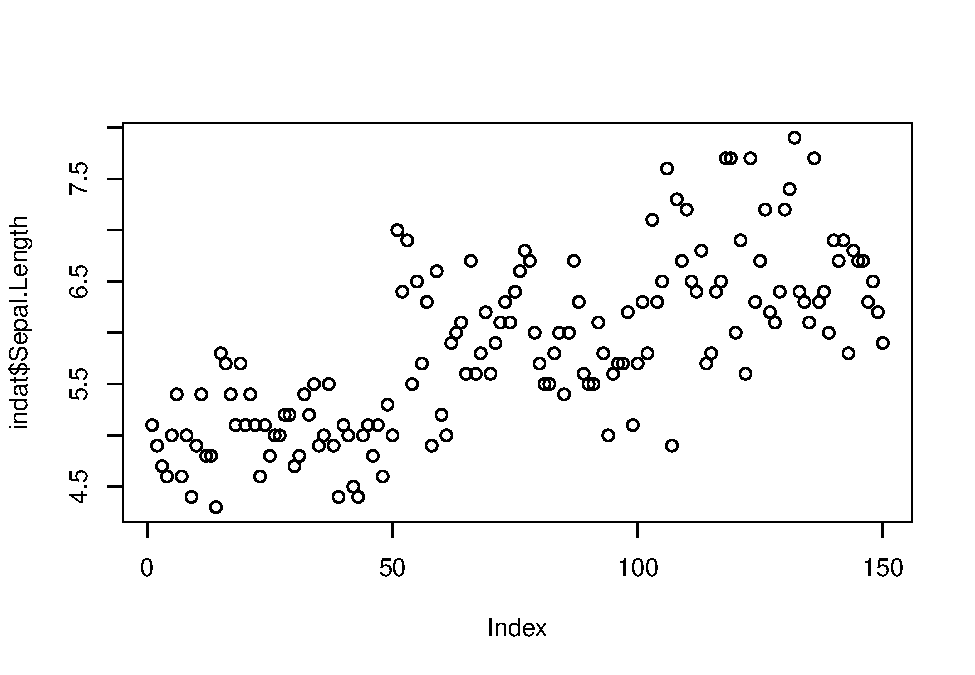
\includegraphics{_main_files/figure-latex/simpleplot-1.pdf}

We now add some labels to a new plot of sepal length as a function of
species (note the use of \texttt{\textasciitilde{}} to mean \emph{as a
function of}; this is also used below when specifying regression models,
where the object on the left of \texttt{\textasciitilde{}} will be the
response variable and the objects on the right explanatory variables)

\begin{Shaded}
\begin{Highlighting}[]
\NormalTok{ys <-}\StringTok{ }\NormalTok{indat}\OperatorTok{$}\NormalTok{Sepal.Length}
\NormalTok{xs <-}\StringTok{ }\NormalTok{indat}\OperatorTok{$}\NormalTok{Species}
\CommentTok{#note use of ~ to represent "as a function of"}
\KeywordTok{plot}\NormalTok{(ys}\OperatorTok{~}\NormalTok{xs, }\DataTypeTok{ylab=}\StringTok{"Sepal Length (in mm)"}\NormalTok{, }\DataTypeTok{main=}\StringTok{"Sepal length by species"}\NormalTok{)}
\end{Highlighting}
\end{Shaded}

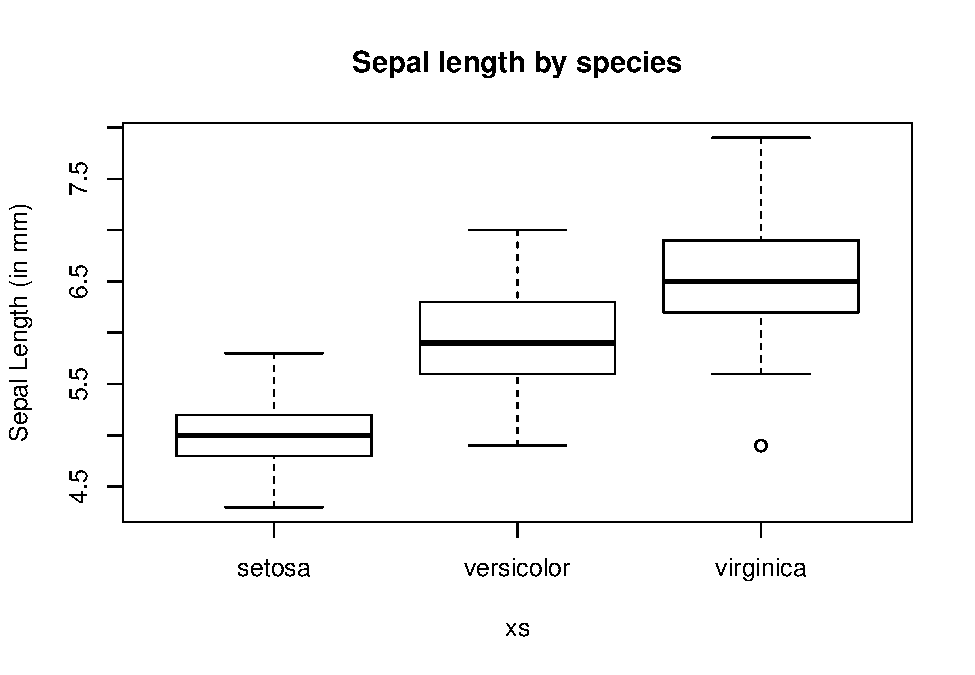
\includegraphics{_main_files/figure-latex/flowerplot-1.pdf}

We can also set the graphic window to hold multiple plots. This is
obtained via argument \texttt{mfrow}, one of the arguments in function
\texttt{par}.\footnote{Note this function controls a much larger number
  of graphical parameters. You can take a look at its help file to get a
  feel for how many and what kind of control it allows you.} An example
follows, in which we leverage on the use of function \texttt{with} to
avoid having to constantly use \texttt{indat\$} to tell R where the data
can be found.

\begin{Shaded}
\begin{Highlighting}[]
\CommentTok{#define two rows and 2 columns of plots}
\KeywordTok{par}\NormalTok{(}\DataTypeTok{mfrow=}\KeywordTok{c}\NormalTok{(}\DecValTok{3}\NormalTok{,}\DecValTok{2}\NormalTok{))}
\KeywordTok{with}\NormalTok{(indat, }\KeywordTok{hist}\NormalTok{(Sepal.Length, }\DataTypeTok{main=}\StringTok{""}\NormalTok{))}
\KeywordTok{with}\NormalTok{(indat, }\KeywordTok{hist}\NormalTok{(Sepal.Width, }\DataTypeTok{main=}\StringTok{""}\NormalTok{))}
\KeywordTok{with}\NormalTok{(indat, }\KeywordTok{hist}\NormalTok{(Petal.Length, }\DataTypeTok{main=}\StringTok{""}\NormalTok{))}
\KeywordTok{with}\NormalTok{(indat, }\KeywordTok{hist}\NormalTok{(Petal.Width, }\DataTypeTok{main=}\StringTok{""}\NormalTok{))}
\KeywordTok{with}\NormalTok{(indat, }\KeywordTok{plot}\NormalTok{(Petal.Length, Petal.Width, }\DataTypeTok{pch=}\DecValTok{21}\NormalTok{, }\DataTypeTok{col=}\DecValTok{12}\NormalTok{, }\DataTypeTok{bg=}\DecValTok{3}\NormalTok{))}
\KeywordTok{with}\NormalTok{(indat, }\KeywordTok{plot}\NormalTok{(Sepal.Length, Sepal.Width, }\DataTypeTok{pch=}\DecValTok{16}\NormalTok{, }\DataTypeTok{col=}\DecValTok{3}\NormalTok{))}
\end{Highlighting}
\end{Shaded}

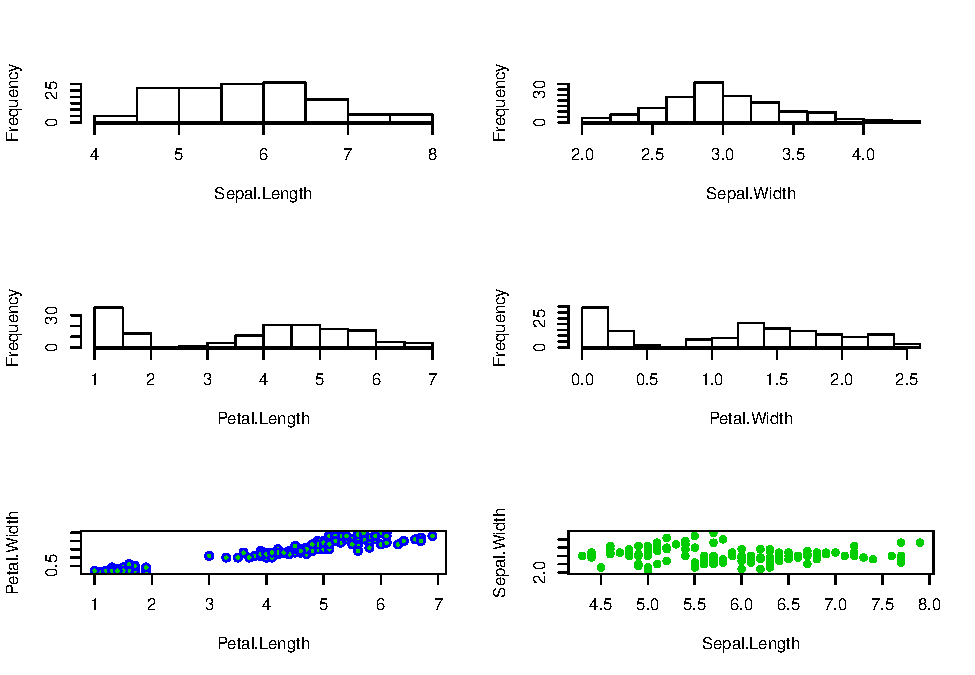
\includegraphics{_main_files/figure-latex/plot2col-1.pdf}

We used argument \texttt{mfrow}, but looking at the help for function
`par gives you an insight to the level of customization one can reach
with respect to these graphical parameters, via dozens of different
arguments.

We can look at the correlation structure between all variables using
function \texttt{pairs()}.

\begin{Shaded}
\begin{Highlighting}[]
\CommentTok{# define two rows and 2 columns of plots}
\KeywordTok{par}\NormalTok{(}\DataTypeTok{mfrow=}\KeywordTok{c}\NormalTok{(}\DecValTok{1}\NormalTok{,}\DecValTok{1}\NormalTok{))}
\KeywordTok{pairs}\NormalTok{(indat)}
\end{Highlighting}
\end{Shaded}

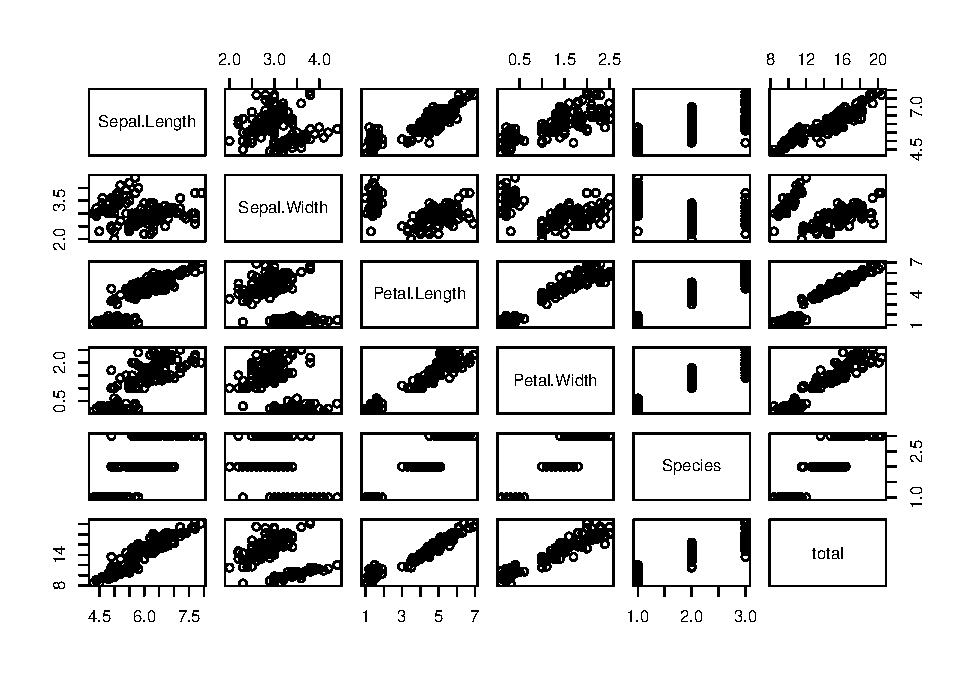
\includegraphics{_main_files/figure-latex/pairs-1.pdf}

\textbf{Task 3}: Using data \texttt{cars}, create a plot that represents
the stopping distances as a function of the speed of cars. Use the
\texttt{points} function to add a special symbol to points corresponding
to cars with speed lower than 15 mph, but distance larger than 70m.
Check out the function \texttt{text} to add text annotations to plots.
Customize axis labels.

\section{Extending basic capabilities via
packages}\label{extending-basic-capabilities-via-packages}

While R base installation includes enough functions that getting
acquainted with them could take several years, many more are available
via the installation of additional packages available online. A package
is just a set of functions and data sets (and the corresponding
documentation plus some additional required files) which usually have
some specific goal. As examples, in our workshop we will be using
packages \texttt{secr} and \texttt{mgcv}, which allow the implementation
of spatially explicit capture recapture (SECR) models and generalized
additive models (GAM), respectively.

Note packages cover a very wide range of applications, and chances are
that at least a package, often more than one, already exists to
implement most kinds of statistical or data processing tasks we might
imagine.

Installing a new package in R requires a call to function
\texttt{install.packages()}. A RStudio shortcut is simply to follow the
\texttt{Tools\textbar{}Install\ packages...} shortcut.

After a package is installed it needs to be loaded to be available. In R
this is done calling function \texttt{library()} with the package name
as an argument. In RStudio this becomes simpler by checking the boxes
under the RStudio tab packages (by default this tab is available on the
bottom right window, along with the Files, Plots, Help and Viewer tabs).

We use \texttt{secr} as an example. Notice, to begin with \texttt{secr}
is not available

\begin{Shaded}
\begin{Highlighting}[]
\NormalTok{?secr}
\end{Highlighting}
\end{Shaded}

\begin{verbatim}
## No documentation for 'secr' in specified packages and libraries:
## you could try '??secr'
\end{verbatim}

Next, we install the package.

\begin{Shaded}
\begin{Highlighting}[]
\KeywordTok{install.packages}\NormalTok{(}\StringTok{"secr"}\NormalTok{)}
\end{Highlighting}
\end{Shaded}

Then, we load the package

\begin{Shaded}
\begin{Highlighting}[]
\KeywordTok{library}\NormalTok{(}\StringTok{"secr"}\NormalTok{)}
\end{Highlighting}
\end{Shaded}

\begin{verbatim}
## This is secr 3.0.1. For overview type ?secr
\end{verbatim}

and finally we check that the functions in it are now loaded

\begin{Shaded}
\begin{Highlighting}[]
\NormalTok{?secr}
\end{Highlighting}
\end{Shaded}

We would now be ready to analyse results from a SECR survey.

\textbf{Task 4}: Run the example code available in the help page from
package \texttt{secr}. Try to understand what is happening: we simulate
some SECR data and we then estimate density based on simulated capture
histories. In particular, look at the simulated density and the
estimated density. This is just a taster for the course to
follow\ldots{}!

\section{Linear regression}\label{linear-regression}

One of the most common type of data analysis is a regression model.
Despite common and conceptually simple, it is a very powerful way to
understand which (and how) of a number of candidate variables, sometimes
referred to covariates, independent or explanatory variables, might
influence a dependent variable, also often referred as the response.
There are many flavours of regression models, from a simple linear
regression to complicated generalized additive mixed models. We do not
wish to present these in any detail, but to introduce you to some
functions that implement these models and the syntax that R uses to
describe them.

Let's start with the basics. You have used the \texttt{cars} data set
above. We use it here again to try to explain the distance a car takes
to stop as a function of its speed. We start with a linear model using
function \texttt{lm()}

\begin{Shaded}
\begin{Highlighting}[]
\KeywordTok{data}\NormalTok{(cars)}
\NormalTok{mylm1 <-}\StringTok{ }\KeywordTok{lm}\NormalTok{(dist}\OperatorTok{~}\NormalTok{speed, }\DataTypeTok{data=}\NormalTok{cars)}
\end{Highlighting}
\end{Shaded}

We have stored the result of fitting the model in object \texttt{mylm1}.
The function \texttt{summary()} can be used to print a summary of the
fit

\begin{Shaded}
\begin{Highlighting}[]
\KeywordTok{summary}\NormalTok{(mylm1)}
\end{Highlighting}
\end{Shaded}

\begin{verbatim}
## 
## Call:
## lm(formula = dist ~ speed, data = cars)
## 
## Residuals:
##     Min      1Q  Median      3Q     Max 
## -29.069  -9.525  -2.272   9.215  43.201 
## 
## Coefficients:
##             Estimate Std. Error t value Pr(>|t|)    
## (Intercept) -17.5791     6.7584  -2.601   0.0123 *  
## speed         3.9324     0.4155   9.464 1.49e-12 ***
## ---
## Signif. codes:  0 '***' 0.001 '**' 0.01 '*' 0.05 '.' 0.1 ' ' 1
## 
## Residual standard error: 15.38 on 48 degrees of freedom
## Multiple R-squared:  0.6511, Adjusted R-squared:  0.6438 
## F-statistic: 89.57 on 1 and 48 DF,  p-value: 1.49e-12
\end{verbatim}

Do not get frightened about all the output. The coefficient associated
with speed tells us what intuition alone would anticipate, the higher
the speed, the larger the distance a car takes to stop. The easier way
to see the relationship is by adding a line to the plot (note this is a
similar plot to what you should have created in task 3 above!). The
predicted relationship is shown in Figure \ref{fig:plotreg}.

\begin{Shaded}
\begin{Highlighting}[]
\NormalTok{xl <-}\StringTok{ "Speed (mph)"}
\NormalTok{yl <-}\StringTok{ "Distance (m)"}
\KeywordTok{plot}\NormalTok{(cars}\OperatorTok{$}\NormalTok{speed, cars}\OperatorTok{$}\NormalTok{dist, }\DataTypeTok{xlab=}\NormalTok{xl, }\DataTypeTok{ylab=}\NormalTok{yl, }\DataTypeTok{ylim=}\KeywordTok{c}\NormalTok{(}\DecValTok{0}\NormalTok{,}\DecValTok{120}\NormalTok{) ,}\DataTypeTok{xlim=}\KeywordTok{c}\NormalTok{(}\DecValTok{0}\NormalTok{,}\DecValTok{30}\NormalTok{))}
\KeywordTok{abline}\NormalTok{(mylm1)}
\end{Highlighting}
\end{Shaded}

\begin{figure}
\centering
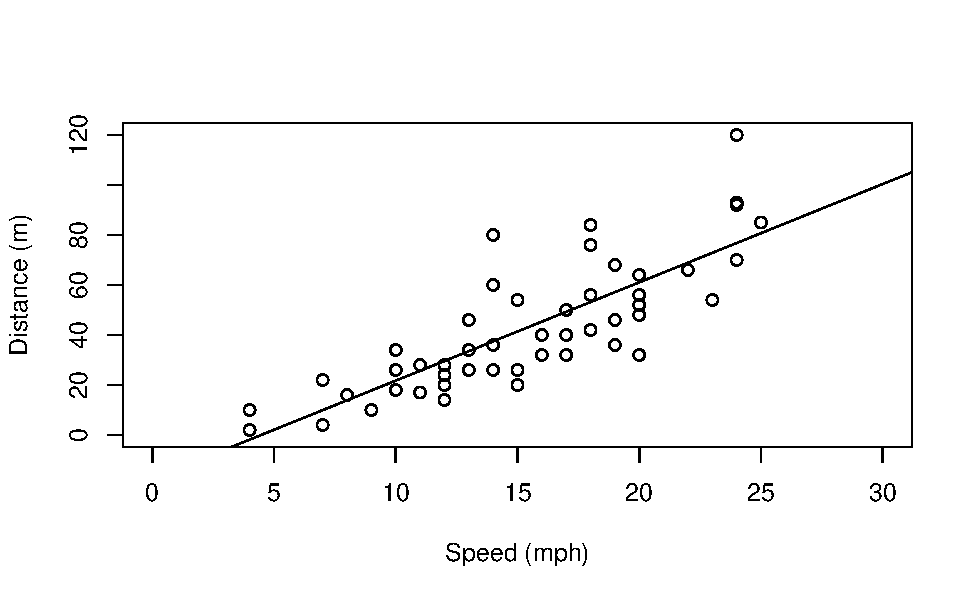
\includegraphics{_main_files/figure-latex/plotreg-1.pdf}
\caption{\label{fig:plotreg}The data and the linear fit added to it.}
\end{figure}

Note how function \texttt{abline()} is used with a linear model as its
first argument and it uses the parameters in said object to add a line
to the plot. The optional arguments \texttt{v} and \texttt{h} are often
very useful to draw vertical and horizontal lines in plots.

\textbf{Task 5}: Use abline to draw dashed lines (tip, use optional
argument \texttt{lty=2}) representing the estimated distance that a car
moving at 16 mph would take to stop.

Note that the line added to the plot represents the distance a car would
take to stop given its speed. Oddly enough, it seems like a car going at
3 mph might take a negative time to stop, which is just plain nonsense.
Why? Because we used a model which does not respect the features of the
data. A stopping distance can not be negative. However, implicit in the
linear model we used, distance is a Gaussian (=normal) random variable.
We can avoid this by using a generalized linear model (GLM). Now the
response can have a range of distributions. An example of such
distribution that takes only positive values is the gamma distribution.
We implement a gamma GLM next

\begin{Shaded}
\begin{Highlighting}[]
\CommentTok{#fit the glm}
\NormalTok{myglm1 <-}\StringTok{ }\KeywordTok{glm}\NormalTok{(dist}\OperatorTok{~}\NormalTok{speed, }\DataTypeTok{data=}\NormalTok{cars, }\DataTypeTok{family=}\KeywordTok{Gamma}\NormalTok{(}\DataTypeTok{link=}\NormalTok{log))}
\CommentTok{#predict using the glm for speeds between 1 and 30}
\NormalTok{predmyglm1 <-}\StringTok{ }\KeywordTok{predict.glm}\NormalTok{(myglm1, }\DataTypeTok{newdata=}\KeywordTok{data.frame}\NormalTok{(}\DataTypeTok{speed=}\DecValTok{1}\OperatorTok{:}\DecValTok{30}\NormalTok{), }
                          \DataTypeTok{type=}\StringTok{"response"}\NormalTok{)}
\end{Highlighting}
\end{Shaded}

Our model now assumes the response has a gamma distribution, and the
link function is the logarithm. The link function allows you to change
how the mean value is related to the covariates. This becomes rather
technical rather fast. Details about glms are naturally beyond the scope
of this tutorial. References like Faraway
(\protect\hyperlink{ref-Faraway2006}{2006}) or Zuur et al.
(\protect\hyperlink{ref-Zuur2009b}{2009}) will provide further details
in an applied context. The predicted relationship is shown in Figure
\ref{fig:plotgam}.

\begin{Shaded}
\begin{Highlighting}[]
\CommentTok{#create a plot}
\KeywordTok{plot}\NormalTok{(cars}\OperatorTok{$}\NormalTok{speed,cars}\OperatorTok{$}\NormalTok{dist, }\DataTypeTok{xlab=}\StringTok{"Speed (mph)"}\NormalTok{, }\DataTypeTok{ylab=}\StringTok{"Distance (m)"}\NormalTok{, }
     \DataTypeTok{ylim=}\KeywordTok{c}\NormalTok{(}\DecValTok{0}\NormalTok{,}\DecValTok{120}\NormalTok{), }\DataTypeTok{xlim=}\KeywordTok{c}\NormalTok{(}\DecValTok{0}\NormalTok{,}\DecValTok{30}\NormalTok{))}
\CommentTok{#add the linear fit}
\KeywordTok{abline}\NormalTok{(mylm1)}
\CommentTok{#and now add the glm predictions}
\KeywordTok{lines}\NormalTok{(}\DecValTok{1}\OperatorTok{:}\DecValTok{30}\NormalTok{, predmyglm1, }\DataTypeTok{col=}\StringTok{"blue"}\NormalTok{, }\DataTypeTok{lwd=}\DecValTok{3}\NormalTok{, }\DataTypeTok{lty=}\DecValTok{3}\NormalTok{)}
\end{Highlighting}
\end{Shaded}

\begin{figure}
\centering
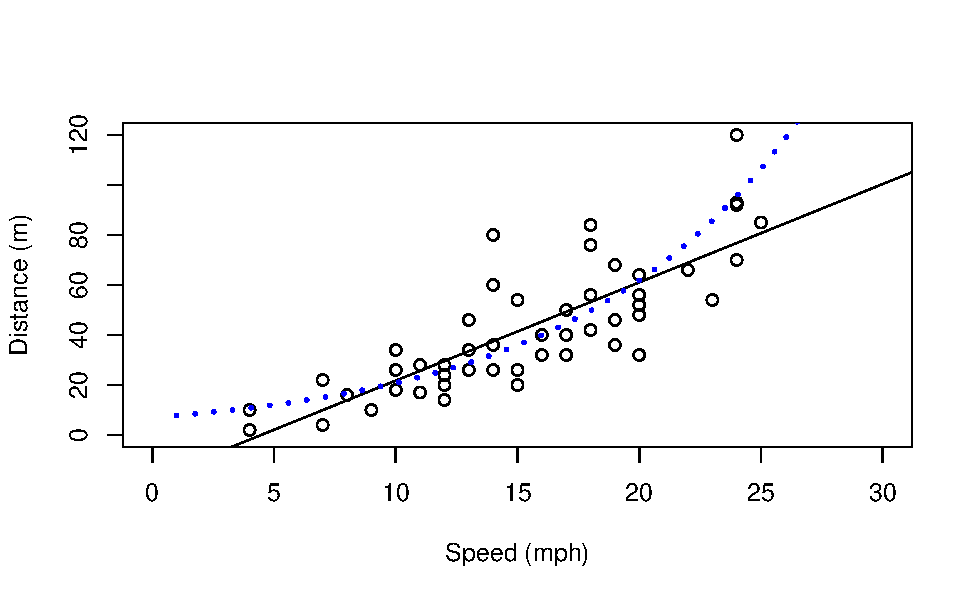
\includegraphics{_main_files/figure-latex/plotgam-1.pdf}
\caption{\label{fig:plotgam}The data and the linear and Gamma glm fits added
to it.}
\end{figure}

However, this glm still requires that the response is linear at some
scale (in this case, on the scale of the link function). Sometimes,
non-linear effects are present. These can be fitted using generalized
additive models. A good introduction to GAMs is provided by Wood
(\protect\hyperlink{ref-Wood2006}{2006}) and Zuur et al.
(\protect\hyperlink{ref-Zuur2009b}{2009}).

So finally we fit a gam model to the same data set. For that we require
library \texttt{mgcv}. The outcome is shown in Figure
\ref{fig:gamfitplot}. Here the fit is not very different from the glm
fit, but under many circumstances a gam might be required over a glm. We
will see such an example in the next few days, when we model the
detectability of beaked whale clicks as a function of distance and angle
(with respect to hydrophones).

\begin{Shaded}
\begin{Highlighting}[]
\CommentTok{#load the mgcv library}
\KeywordTok{library}\NormalTok{(mgcv)}
\end{Highlighting}
\end{Shaded}

\begin{verbatim}
## Loading required package: nlme
\end{verbatim}

\begin{verbatim}
## This is mgcv 1.8-17. For overview type 'help("mgcv-package")'.
\end{verbatim}

\begin{Shaded}
\begin{Highlighting}[]
\CommentTok{#fit the gam}
\NormalTok{mygam1 <-}\StringTok{ }\KeywordTok{gam}\NormalTok{(dist}\OperatorTok{~}\KeywordTok{s}\NormalTok{(speed), }\DataTypeTok{data=}\NormalTok{cars, }\DataTypeTok{family=}\KeywordTok{Gamma}\NormalTok{(}\DataTypeTok{link=}\NormalTok{log))}
\CommentTok{#predict using the glm for speeds between 1 and 30}
\NormalTok{predmygam1 <-}\StringTok{ }\KeywordTok{predict}\NormalTok{(mygam1, }\DataTypeTok{newdata=}\KeywordTok{data.frame}\NormalTok{(}\DataTypeTok{speed=}\DecValTok{1}\OperatorTok{:}\DecValTok{30}\NormalTok{), }\DataTypeTok{type=}\StringTok{"response"}\NormalTok{)}
\end{Highlighting}
\end{Shaded}

\begin{Shaded}
\begin{Highlighting}[]
\CommentTok{#create a plot}
\KeywordTok{plot}\NormalTok{(cars}\OperatorTok{$}\NormalTok{speed, cars}\OperatorTok{$}\NormalTok{dist, }\DataTypeTok{xlab=}\StringTok{"Speed (mph)"}\NormalTok{, }\DataTypeTok{ylab=}\StringTok{"Distance (m)"}\NormalTok{, }
     \DataTypeTok{ylim=}\KeywordTok{c}\NormalTok{(}\DecValTok{0}\NormalTok{,}\DecValTok{120}\NormalTok{), }\DataTypeTok{xlim=}\KeywordTok{c}\NormalTok{(}\DecValTok{0}\NormalTok{,}\DecValTok{30}\NormalTok{))}
\CommentTok{#add the linear fit}
\KeywordTok{abline}\NormalTok{(mylm1)}
\CommentTok{#and now add the glm predictions}
\KeywordTok{lines}\NormalTok{(}\DecValTok{1}\OperatorTok{:}\DecValTok{30}\NormalTok{, predmyglm1, }\DataTypeTok{col=}\StringTok{"blue"}\NormalTok{, }\DataTypeTok{lwd=}\DecValTok{3}\NormalTok{, }\DataTypeTok{lty=}\DecValTok{3}\NormalTok{)}
\KeywordTok{lines}\NormalTok{(}\DecValTok{1}\OperatorTok{:}\DecValTok{30}\NormalTok{, predmygam1, }\DataTypeTok{col=}\StringTok{"green"}\NormalTok{, }\DataTypeTok{lwd=}\DecValTok{3}\NormalTok{, }\DataTypeTok{lty=}\DecValTok{2}\NormalTok{)}
\end{Highlighting}
\end{Shaded}

\begin{figure}
\centering
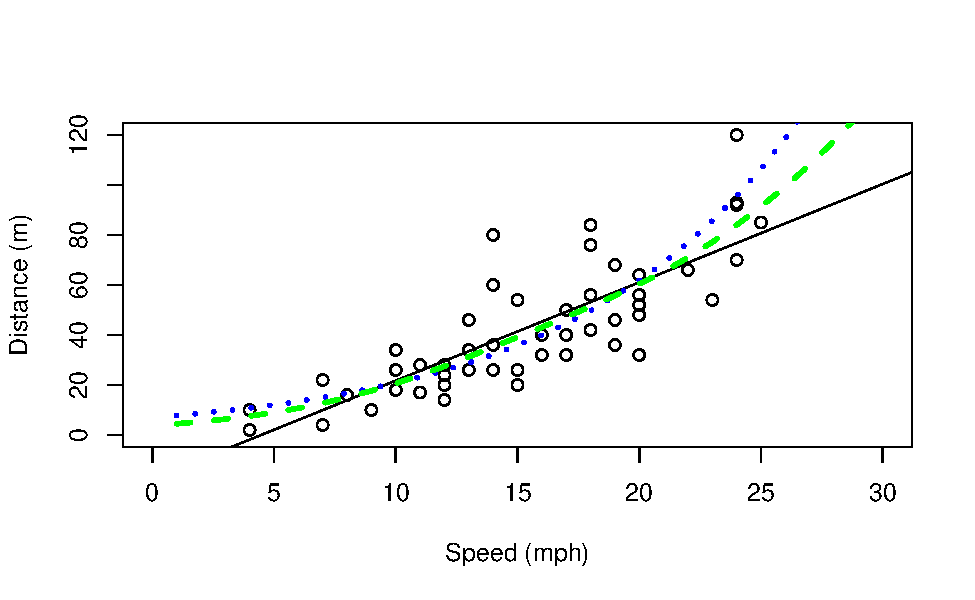
\includegraphics{_main_files/figure-latex/gamfitplot-1.pdf}
\caption{\label{fig:gamfitplot}The data and the linear and Gamma glm and gam
fits added to it.}
\end{figure}

\section{Some advanced capabilities of
R}\label{some-advanced-capabilities-of-r}

\subsection{Simulation and random number
generation}\label{simulation-and-random-number-generation}

Another powerful use of R is for simulation. To this end, R has the
ability to simulate random deviates from a large number of
distributions. Perhaps the more useful and commonly used are the uniform
and the Gaussian distributions. We now create 50 random deviates from
each of these, as well as some Poisson deviates, for illustration

\begin{Shaded}
\begin{Highlighting}[]
\CommentTok{#define two rows and 2 columns of plots}
\NormalTok{rdnorm <-}\StringTok{ }\KeywordTok{rnorm}\NormalTok{(}\DecValTok{50}\NormalTok{,}\DataTypeTok{mean=}\DecValTok{20}\NormalTok{,}\DataTypeTok{sd=}\DecValTok{3}\NormalTok{)}
\NormalTok{rdunif <-}\StringTok{ }\KeywordTok{runif}\NormalTok{(}\DecValTok{50}\NormalTok{,}\DataTypeTok{min=}\DecValTok{3}\NormalTok{,}\DataTypeTok{max=}\DecValTok{6}\NormalTok{)}
\NormalTok{rdpois <-}\StringTok{ }\KeywordTok{rpois}\NormalTok{(}\DecValTok{50}\NormalTok{,}\DataTypeTok{lambda=}\DecValTok{6}\NormalTok{)}
\end{Highlighting}
\end{Shaded}

R can create random numbers from many different distributions (see
help(Distributions) for a list) -- the relevant functions generally
start with r and then an abbreviated distribution name (rbinom, rexp,
rgeom, etc). Additionally, R also includes the ability to obtain the
density function, distribution function and quantile function via the
\texttt{d}+name, \texttt{p}+name and \texttt{q}+name functions. As an
example, the Gaussian function usage of these functions is presented
below

\begin{Shaded}
\begin{Highlighting}[]
\KeywordTok{dnorm}\NormalTok{(}\DecValTok{0}\NormalTok{,}\DataTypeTok{mean=}\DecValTok{0}\NormalTok{,}\DataTypeTok{sd=}\DecValTok{1}\NormalTok{)}
\end{Highlighting}
\end{Shaded}

\begin{verbatim}
## [1] 0.3989423
\end{verbatim}

\begin{Shaded}
\begin{Highlighting}[]
\KeywordTok{pnorm}\NormalTok{(}\DecValTok{0}\NormalTok{,}\DataTypeTok{mean=}\DecValTok{0}\NormalTok{,}\DataTypeTok{sd=}\DecValTok{1}\NormalTok{)}
\end{Highlighting}
\end{Shaded}

\begin{verbatim}
## [1] 0.5
\end{verbatim}

\begin{Shaded}
\begin{Highlighting}[]
\KeywordTok{qnorm}\NormalTok{(}\FloatTok{0.975}\NormalTok{,}\DataTypeTok{mean=}\DecValTok{0}\NormalTok{,}\DataTypeTok{sd=}\DecValTok{1}\NormalTok{)}
\end{Highlighting}
\end{Shaded}

\begin{verbatim}
## [1] 1.959964
\end{verbatim}

\textbf{Task 6}: Using what you have learnt here, create two histograms,
one of 50, another of 5000, random deviates from a Gaussian
distribution, using the optional argument \texttt{freq=FALSE} (leading
to an estimate of the density function). Then add a line to the plot
that represents the true underlying density (tip, you can use function
\texttt{dnorm()}), and comment on the results.

\subsection{Writing your own
functions}\label{writing-your-own-functions}

While the above functions, and the many more available, make R a very
useful tool, there are sometimes problems which require a special tool.
For these, we can create our own functions. Note this is an advanced
topic.

The way of doing that follows a specific syntax

\begin{verbatim}
> name <- function(arg1,arg2,...) {what the function does goes here}
\end{verbatim}

As an example, we create a function that returns the sum of its
arguments:

\begin{Shaded}
\begin{Highlighting}[]
\NormalTok{myfun <-}\StringTok{ }\ControlFlowTok{function}\NormalTok{(i,j)\{}
\NormalTok{  myres <-}\StringTok{ }\NormalTok{i }\OperatorTok{+}\StringTok{ }\NormalTok{j}
  \KeywordTok{return}\NormalTok{(myres)}
\NormalTok{\}}
\end{Highlighting}
\end{Shaded}

\textbf{Task 7}: create a function called \texttt{mystats()} which
returns the mean, variance, maximum and minimum of the first argument (a
vector). Then, update your function such that it can also return the
mean excluding the negative numbers.

\section{Wrap up}\label{wrap-up}

A full introduction to R course could take an entire week. A full course
in regression modelling with R could take an entire semester. A full
course of data analysis in R could take a life time.

Our objective with this tutorial was simply to introduce you to R such
that when we use R in the next few days, the commands do not look too
esoteric. Nonetheless, this material as well as the references provided
should constitute a good basis to learn R further if you so desire.
Beginners find the learning curve is often steep, but once mastered, R
simplifies enormously the task of statistical data analysis.

\begin{Shaded}
\begin{Highlighting}[]
\CommentTok{#cleaning the workspace}
\KeywordTok{rm}\NormalTok{(}\DataTypeTok{list =} \KeywordTok{ls}\NormalTok{())}
\end{Highlighting}
\end{Shaded}

\chapter{analyse simulated data set}\label{analyse-simulated-data-set}

\section{Laura to prepare}\label{laura-to-prepare}

\chapter{Problem datasets}\label{problem-datasets}

\section{Len to prepare}\label{len-to-prepare}

\subsection{Blue monkey data set}\label{blue-monkey-data-set}

\begin{itemize}
\tightlist
\item
  \href{Difficult\%20data/D7BlueMonkey\%20-\%20Demo\%203.zip}{Distance 7
  project}
\item
  \href{Difficult\%20data/BlueMonkey.csv}{Data as csv for R analysis}
\end{itemize}

\subsection{Odd spike data set}\label{odd-spike-data-set}

\begin{itemize}
\tightlist
\item
  \href{Difficult\%20data/D7OddSpike\%20-\%20Demo\%202.zip}{Distance 7
  project}
\item
  \href{Difficult\%20data/Oddspike.r}{R script to manufacture and
  conduct analysis}
\end{itemize}

\chapter{Creating distance sampling simulations using
DSsim}\label{creating-distance-sampling-simulations-using-dssim}

\begin{quote}
Assumes home directory is directory in which exercise has been expanded
\end{quote}

\section{Aim}\label{aim}

The aim of this exercise is to run simulations which will allow you to
compare three different survey designs for a specific population. You
should judge these designs on their accuracy and precision.

You will also need the following R packages installed on your machine:
DSsim, shapefiles, splancs and mrds. Now examine the other files and
folders in the ``DSsim Exercise'' folder. There are three files starting
with the name ``Region'' and ending with .dbf, .shp and .shx, these
files make up the shapefile for the survey region. The
``density.surface.robj'' file is the density surface for the survey
region. The ``Survey Transects'' folder contains a folder for each of
the designs you are asked to look at, these contain the transect
shapefiles. The ``Results'' folder contains the results from 999
replications as this can take a good few hours to run. To setup the
workspace first load the libraries DSsim and shapefiles, loading these
two will automatically make splancs and mrds available.

\begin{Shaded}
\begin{Highlighting}[]
\KeywordTok{library}\NormalTok{(DSsim)}
\KeywordTok{library}\NormalTok{(shapefiles)}
\end{Highlighting}
\end{Shaded}

\section{Create a region object}\label{create-a-region-object}

Read the Region shapefile into R using the read.shapefile function from
the shapefiles library.

\begin{Shaded}
\begin{Highlighting}[]
\NormalTok{region.shapefile <-}\StringTok{ }\KeywordTok{read.shapefile}\NormalTok{(}\StringTok{"Region"}\NormalTok{)}
\end{Highlighting}
\end{Shaded}

Next you are going to create the region object using this shapefile. As
there are no strata you only need to provide a name for your survey
region and the units which are in metres (m). The survey region is
displayed in Figure \ref{fig:finishreg}.

\begin{Shaded}
\begin{Highlighting}[]
\NormalTok{region <-}\StringTok{ }\KeywordTok{make.region}\NormalTok{(}\DataTypeTok{region.name =} \StringTok{"Survey Region"}\NormalTok{, }\DataTypeTok{units =} \StringTok{"m"}\NormalTok{, }
                      \DataTypeTok{shapefile =}\NormalTok{ region.shapefile)}
\KeywordTok{plot}\NormalTok{(region, }\DataTypeTok{plot.units =} \StringTok{"km"}\NormalTok{)}
\end{Highlighting}
\end{Shaded}

\begin{figure}
\centering
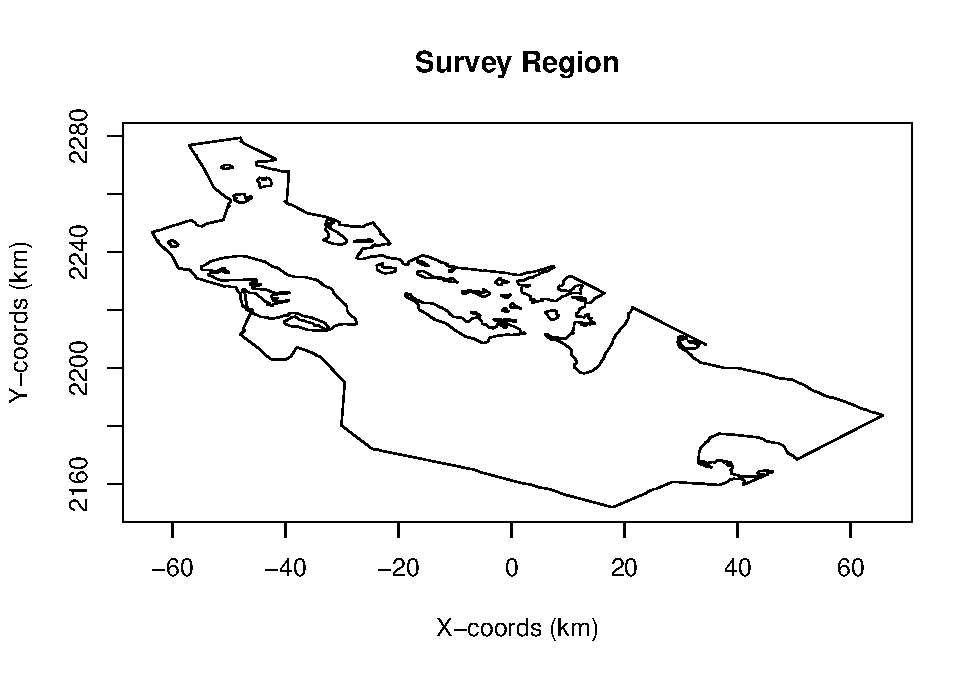
\includegraphics{_main_files/figure-latex/finishreg-1.pdf}
\caption{\label{fig:finishreg}Study region for simulation}
\end{figure}

\section{Create a density object}\label{create-a-density-object}

You are now going to create a density object within this region. For the
purposes of this exercise a density surface has already been created and
can be loaded as follows:

\begin{Shaded}
\begin{Highlighting}[]
\KeywordTok{load}\NormalTok{(}\StringTok{"density.surface.robj"}\NormalTok{)}
\end{Highlighting}
\end{Shaded}

You will see that an object called ``density.surface'' has appeared in
the workspace. This object is a list with one element (if the region had
been divided up into strata then this list would contain an element for
each strata). To have a look at what the density surface data look like
type \texttt{head(density.surface{[}{[}1{]}{]})}. You can see that it is
a data set of x and y locations and the densities at each point.

To create the density object you will need to provide the density
surface, the region object for which it was created and the grid spacing
that was used. I used a grid spacing of 1,000 m in both the x and y
directions to create this density surface. The density surface
describing animal distribution is shown in Figure 4.2.

\begin{Shaded}
\begin{Highlighting}[]
\NormalTok{pop.density <-}\StringTok{ }\KeywordTok{make.density}\NormalTok{(}\DataTypeTok{region =}\NormalTok{ region, }\DataTypeTok{density.surface =}\NormalTok{ density.surface, }
                            \DataTypeTok{x.space =} \DecValTok{1000}\NormalTok{, }\DataTypeTok{y.space =} \DecValTok{1000}\NormalTok{) }
\KeywordTok{plot}\NormalTok{(pop.density, }\DataTypeTok{plot.units =} \StringTok{"km"}\NormalTok{)}
\KeywordTok{plot}\NormalTok{(region, }\DataTypeTok{add =} \OtherTok{TRUE}\NormalTok{)}
\end{Highlighting}
\end{Shaded}

\begin{figure}
\centering
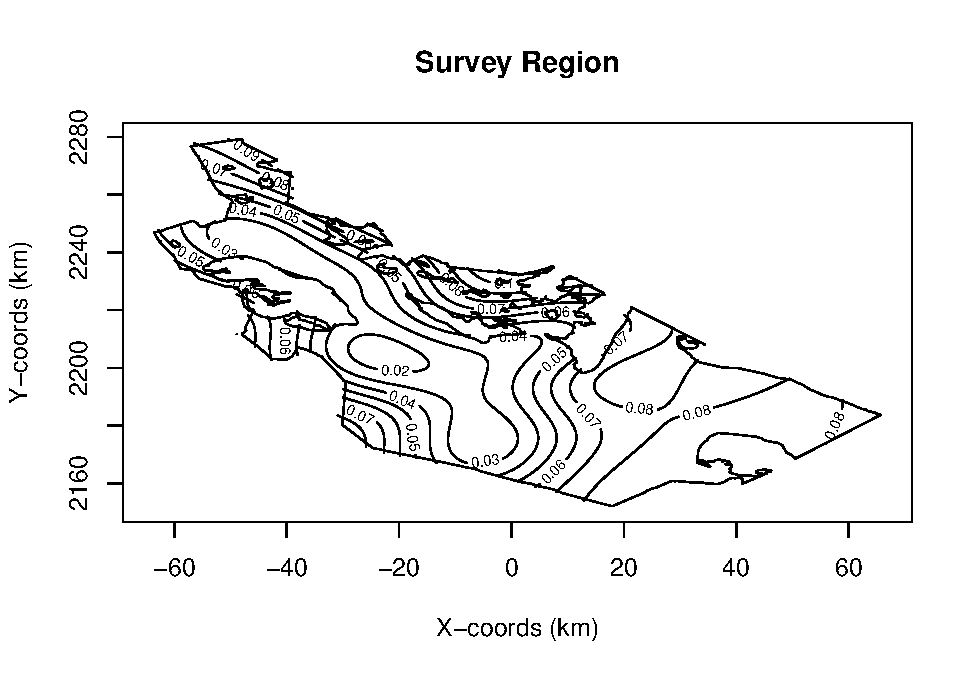
\includegraphics{_main_files/figure-latex/popden-1.pdf}
\caption{\label{fig:popden}Study region with animal density superimposed
Note lower density near the trail system}
\end{figure}

Optionally, the following code can be used to define your own density
surface. Firstly the density object is created with a constant value,
then high and low spots can be added with varying radii of influence.
The sigma parameter is used to calculate a Gaussian decay around the
central point.

\begin{Shaded}
\begin{Highlighting}[]
\NormalTok{alternative.density <-}\StringTok{ }\KeywordTok{make.density}\NormalTok{(}\DataTypeTok{region =}\NormalTok{ region, }\DataTypeTok{x.space =} \DecValTok{1000}\NormalTok{, }
                                    \DataTypeTok{y.space =} \DecValTok{1000}\NormalTok{, }\DataTypeTok{constant =} \FloatTok{0.4e-7}\NormalTok{)}

\NormalTok{alternative.density <-}\StringTok{ }\KeywordTok{add.hotspot}\NormalTok{(alternative.density, }\DataTypeTok{centre =} \KeywordTok{c}\NormalTok{(}\OperatorTok{-}\DecValTok{2500}\NormalTok{, }\DecValTok{2224000}\NormalTok{), }
                                   \DataTypeTok{sigma =} \DecValTok{10000}\NormalTok{, }\DataTypeTok{amplitude =} \FloatTok{0.1e-7}\NormalTok{)}
\NormalTok{alternative.density <-}\StringTok{ }\KeywordTok{add.hotspot}\NormalTok{(alternative.density, }\DataTypeTok{centre =} \KeywordTok{c}\NormalTok{(}\DecValTok{0}\NormalTok{, }\DecValTok{2184000}\NormalTok{), }
                                   \DataTypeTok{sigma =} \DecValTok{18000}\NormalTok{, }\DataTypeTok{amplitude =} \OperatorTok{-}\FloatTok{0.5e-8}\NormalTok{)}
\end{Highlighting}
\end{Shaded}

\section{Creating population description and detectability
objects}\label{creating-population-description-and-detectability-objects}

For this exercise we will fix the population size at 1500 individuals.
To do this set N = 1500 and tell it to generate exactly this number of
individuals (fixed.N = TRUE).

\begin{Shaded}
\begin{Highlighting}[]
\NormalTok{pop.description <-}\StringTok{ }\KeywordTok{make.population.description}\NormalTok{(}\DataTypeTok{region.obj =}\NormalTok{ region, }
                                               \DataTypeTok{density.obj =}\NormalTok{ pop.density, }
                                               \DataTypeTok{N =} \DecValTok{1500}\NormalTok{, }\DataTypeTok{fixed.N =} \OtherTok{TRUE}\NormalTok{)}
\end{Highlighting}
\end{Shaded}

We will now describe the detectability of the population using a
half-normal function with a sigma (scale.param) of 500 m and a
truncation distance of 1000 m. This means that around 2/3 of the
detections will be made within 500 m of the transect and we will exclude
anything sighted further than 1000 m perpendicular distance from the
transect.

\begin{Shaded}
\begin{Highlighting}[]
\NormalTok{detect <-}\StringTok{ }\KeywordTok{make.detectability}\NormalTok{(}\DataTypeTok{key.function =} \StringTok{"hn"}\NormalTok{, }\DataTypeTok{scale.param =} \DecValTok{500}\NormalTok{, }\DataTypeTok{truncation =} \DecValTok{1000}\NormalTok{)}
\end{Highlighting}
\end{Shaded}

\section{Creating the survey design
object}\label{creating-the-survey-design-object}

We will now create a design object. For now concentrate on the
subjective design, we will come back to the parallel and zigzag designs
later. The subjective design was based on using some \textbf{existing
paths} to make the survey easier to carry out. Additional transects were
then added to achieve a more even coverage of the survey region.

NOTE: The path argument to describe where the files are located must
match your previous settings add ``/Survey Transects/Subjective
Design''.

\begin{Shaded}
\begin{Highlighting}[]
\NormalTok{subjective.design <-}\StringTok{ }\KeywordTok{make.design}\NormalTok{(}\DataTypeTok{transect.type =} \StringTok{"Line"}\NormalTok{, }
                                 \DataTypeTok{design.details =} \KeywordTok{c}\NormalTok{(}\StringTok{"user specified"}\NormalTok{), }
                                 \DataTypeTok{region =}\NormalTok{ region, }
                                 \DataTypeTok{plus.sampling =} \OtherTok{FALSE}\NormalTok{, }
                                 \DataTypeTok{path =} \StringTok{"Survey Transects/Subjective Design"}\NormalTok{)}
\end{Highlighting}
\end{Shaded}

\section{Creating the analyses
object}\label{creating-the-analyses-object}

The final thing we need to do before creating the simulation object is
describe the analyses we wish to carry out on the simulated data. Let's
try letting it choose between a half-normal and a hazard rate model
based on the AIC values.

\begin{Shaded}
\begin{Highlighting}[]
\NormalTok{ddf.analyses <-}\StringTok{ }\KeywordTok{make.ddf.analysis.list}\NormalTok{(}
                \DataTypeTok{dsmodel =} \KeywordTok{list}\NormalTok{(}\OperatorTok{~}\KeywordTok{cds}\NormalTok{(}\DataTypeTok{key =} \StringTok{"hn"}\NormalTok{, }\DataTypeTok{formula =} \OperatorTok{~}\DecValTok{1}\NormalTok{), }\CommentTok{#half-normal model}
                               \OperatorTok{~}\KeywordTok{cds}\NormalTok{(}\DataTypeTok{key =} \StringTok{"hr"}\NormalTok{, }\DataTypeTok{formula =} \OperatorTok{~}\DecValTok{1}\NormalTok{)),  }\CommentTok{#hazard rate model}
                \DataTypeTok{method =} \StringTok{"ds"}\NormalTok{, }\DataTypeTok{criteria =} \StringTok{"AIC"}\NormalTok{, }\DataTypeTok{truncation =} \DecValTok{1000}\NormalTok{)}
\end{Highlighting}
\end{Shaded}

\section{Creating the simulation
object}\label{creating-the-simulation-object}

We can finally put it all together and have a look at some example
populations, transects and survey data. I suggest you set the number of
repetitions (reps) to be fairly low or else it will take a long time to
run. For the subjective design you need to specify that it will be using
the same set of transects each time, single.transect.set = TRUE.

\begin{Shaded}
\begin{Highlighting}[]
\NormalTok{my.simulation.subjective <-}\StringTok{ }\KeywordTok{make.simulation}\NormalTok{(}\DataTypeTok{reps =} \DecValTok{10}\NormalTok{, }
                                            \DataTypeTok{single.transect.set =} \OtherTok{TRUE}\NormalTok{, }
                                            \DataTypeTok{region.obj =}\NormalTok{ region, }
                                            \DataTypeTok{design.obj =}\NormalTok{ subjective.design, }
                                            \DataTypeTok{population.description.obj =}\NormalTok{ pop.description,}
                                            \DataTypeTok{detectability.obj =}\NormalTok{ detect, }
                                            \DataTypeTok{ddf.analyses.list =}\NormalTok{ ddf.analyses)}
\end{Highlighting}
\end{Shaded}

Before running the simulation it is a good idea to have a check to see
that it is doing what you want. The function \texttt{check.sim.setup()}
will allow you to investigate the simulation properties. Having created
a population, transects, survey and detections, the function plots them
to assure you are happy with the simulation structure.

Let's check our subjective design simulation, see Figure
\ref{fig:plotsimul}.

\begin{Shaded}
\begin{Highlighting}[]
\KeywordTok{check.sim.setup}\NormalTok{(my.simulation.subjective)}
\end{Highlighting}
\end{Shaded}

\begin{figure}
\centering
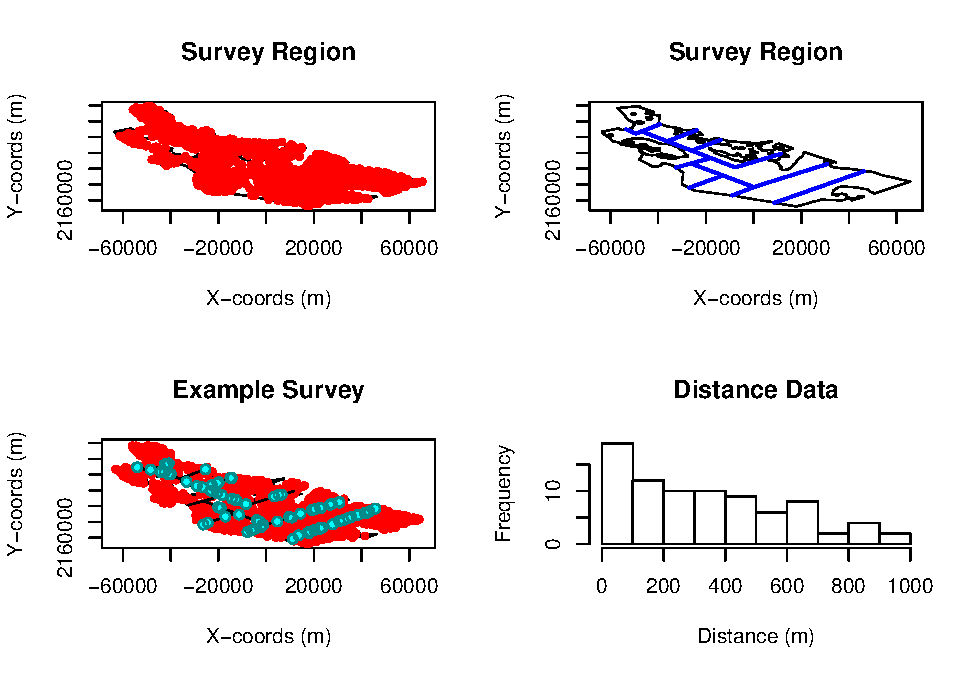
\includegraphics{_main_files/figure-latex/plotsimul-1.pdf}
\caption{\label{fig:plotsimul}Region, population, transects, detections}
\end{figure}

Once you are happy it is time to run the simulation. Please be patient
as it will take a few minutes to complete.

\begin{Shaded}
\begin{Highlighting}[]
\NormalTok{my.simulation.subjective  <-}\StringTok{ }\KeywordTok{run}\NormalTok{(my.simulation.subjective)}
\KeywordTok{summary}\NormalTok{(my.simulation.subjective, }\DataTypeTok{description.summary =} \OtherTok{FALSE}\NormalTok{)}
\end{Highlighting}
\end{Shaded}

\section{Now for the automated designs: Parallel
lines}\label{now-for-the-automated-designs-parallel-lines}

You will need to create a new simulation each with a new design object
for the parallel design. The other objects (region, density, population
description etc.) should be left the same.

NOTE: We now wish different transects to be used on each repetition
(\texttt{single.transect.set\ =\ FALSE}).

\begin{Shaded}
\begin{Highlighting}[]
\NormalTok{parallel.design <-}\StringTok{ }\KeywordTok{make.design}\NormalTok{(}\DataTypeTok{transect.type =} \StringTok{"Line"}\NormalTok{,}
                               \DataTypeTok{design.details =} \KeywordTok{c}\NormalTok{(}\StringTok{"Parallel"}\NormalTok{,}\StringTok{"Systematic"}\NormalTok{),}
                               \DataTypeTok{region.obj =}\NormalTok{ region, }\DataTypeTok{design.axis =} \DecValTok{45}\NormalTok{,}
                               \DataTypeTok{spacing =} \DecValTok{12000}\NormalTok{, }\DataTypeTok{plus.sampling =} \OtherTok{FALSE}\NormalTok{,}
                               \DataTypeTok{path =} \StringTok{"Survey Transects/Parallel Design"}\NormalTok{)}

\NormalTok{my.simulation.parallel <-}\StringTok{ }\KeywordTok{make.simulation}\NormalTok{(}\DataTypeTok{reps =} \DecValTok{10}\NormalTok{, }
                                          \DataTypeTok{single.transect.set =} \OtherTok{FALSE}\NormalTok{, }
                                          \DataTypeTok{region.obj =}\NormalTok{ region, }
                                          \DataTypeTok{design.obj =}\NormalTok{ parallel.design, }
                                          \DataTypeTok{population.description.obj =}\NormalTok{ pop.description,}
                                          \DataTypeTok{detectability.obj =}\NormalTok{ detect,}
                                          \DataTypeTok{ddf.analyses.list =}\NormalTok{ ddf.analyses)}
\end{Highlighting}
\end{Shaded}

Having created the features of the simulation, we want to check features
of the simulation have been correctly specified, see Figure
\ref{fig:parallelcheck}.

\begin{Shaded}
\begin{Highlighting}[]
\KeywordTok{check.sim.setup}\NormalTok{(my.simulation.parallel)}
\end{Highlighting}
\end{Shaded}

\begin{figure}
\centering
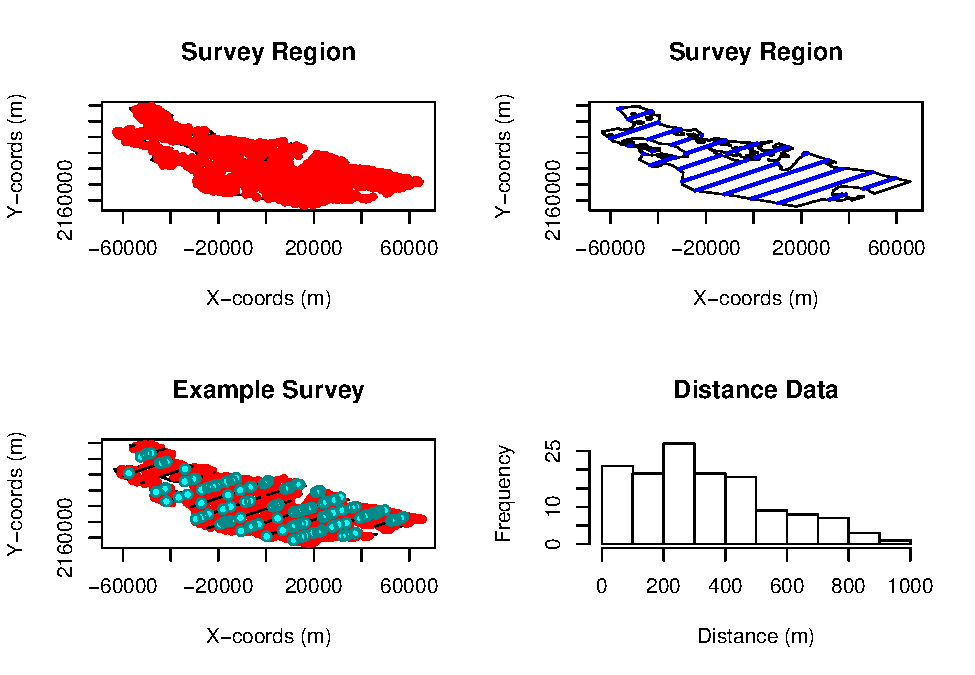
\includegraphics{_main_files/figure-latex/parallelcheck-1.pdf}
\caption{\label{fig:parallelcheck}Check setup of parallel transect design
simulation}
\end{figure}

When satisfied with this simulation setup, you would proceed to run your
parallel design simulation.

\begin{Shaded}
\begin{Highlighting}[]
\NormalTok{my.simulation.parallel  <-}\StringTok{ }\KeywordTok{run}\NormalTok{(my.simulation.parallel)}
\KeywordTok{summary}\NormalTok{(my.simulation.parallel, }\DataTypeTok{description.summary =} \OtherTok{FALSE}\NormalTok{)}
\end{Highlighting}
\end{Shaded}

\subsection{ZigZag survey design}\label{zigzag-survey-design}

Now have a go at creating and running a simulation using the equal
spaced zigzag design transects in the ``Zigzag Design'' folder. The
spacing used to generate these was 8250m on a design axis of 135
degrees. Use \texttt{?make.design} for help.

Having created the features of the simulation, check the features of the
simulation have been correctly specified (Fig. \ref{fig:zigzagcheck}).

\begin{figure}
\centering
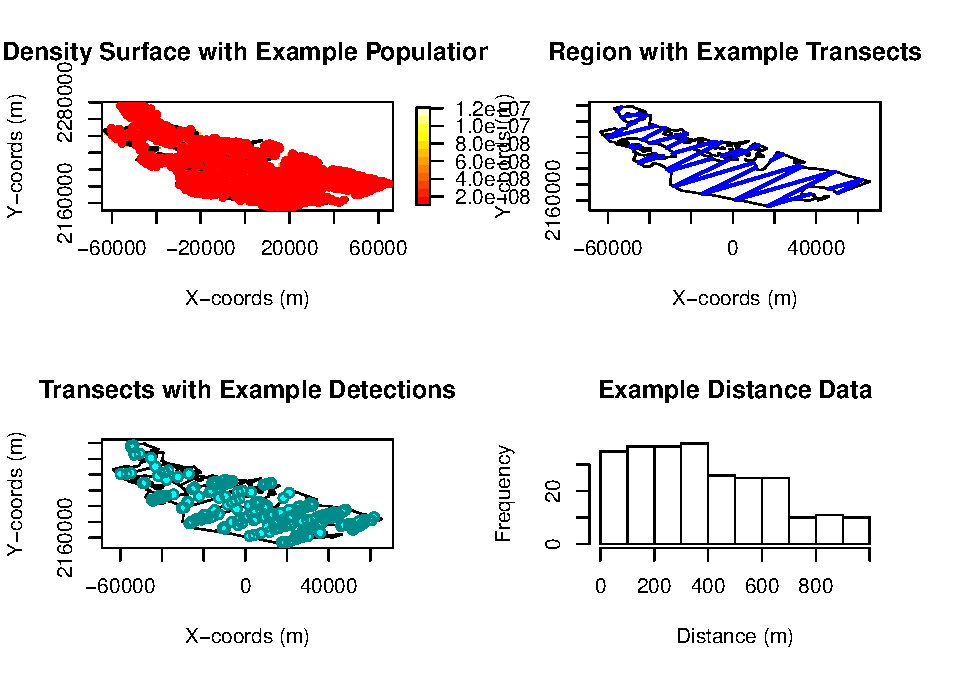
\includegraphics{_main_files/figure-latex/zigzagcheck-1.pdf}
\caption{\label{fig:zigzagcheck}Check setup of zigzag transect design
simulation}
\end{figure}

When satisfied with this simulation setup, you would proceed to run your
zigzag design simulation.

\begin{Shaded}
\begin{Highlighting}[]
\NormalTok{my.simulation.zigzag  <-}\StringTok{ }\KeywordTok{run}\NormalTok{(my.simulation.zigzag)}
\KeywordTok{summary}\NormalTok{(my.simulation.zigzag)}
\end{Highlighting}
\end{Shaded}

\section{Results from 999
repetitions}\label{results-from-999-repetitions}

I ran each of these simulations 999 times and stored the simulations as
r objects. Load these into the R workspace using the following code:

\begin{Shaded}
\begin{Highlighting}[]
\KeywordTok{load}\NormalTok{(}\StringTok{"Results/simulation.subjective.robj"}\NormalTok{)}
\KeywordTok{load}\NormalTok{(}\StringTok{"Results/simulation.parallel.robj"}\NormalTok{)}
\KeywordTok{load}\NormalTok{(}\StringTok{"Results/simulation.zigzag.robj"}\NormalTok{)}
\end{Highlighting}
\end{Shaded}

The objects \texttt{simulation.subjective}, \texttt{simulation.parallel}
and \texttt{simulation.zigzag} will now be in your workspace. Have a
look at the results using the \texttt{summary()} function and use them
to fill in the table below, Figure 4.5.

\begin{Shaded}
\begin{Highlighting}[]
\KeywordTok{summary}\NormalTok{(simulation.subjective)}
\KeywordTok{summary}\NormalTok{(simulation.parallel)}
\KeywordTok{summary}\NormalTok{(simulation.zigzag)}
\end{Highlighting}
\end{Shaded}

Which survey design would you recommend? Why?\\
What would happen if our assumptions about animal distribution were
incorrect?

\begin{figure}
\centering
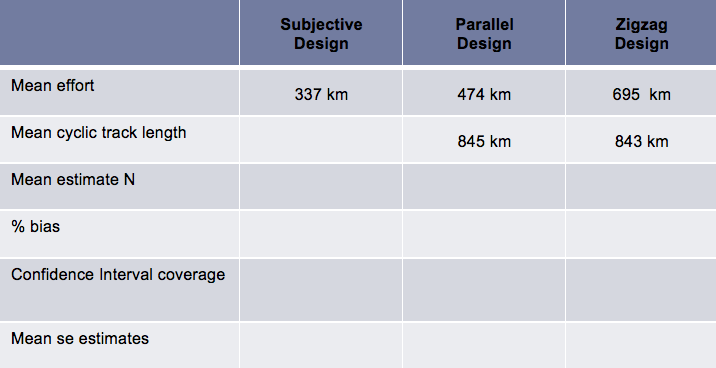
\includegraphics{images/results.png}
\caption{Results Table}
\end{figure}

\section{Running distance sampling simulations using Distance
7.1}\label{running-distance-sampling-simulations-using-distance-7.1}

If you would like to investigate different designs then these can be
created and used in simulations in Distance 7.1. Note that currently the
simulation options in Distance 7.1 are somewhat more restricted than in
DSsim.

We have created a Distance project based on the scenario just described
and setup the systematic parallel and equal spaced zigzag designs as
specified above. This project is named \texttt{DSsimExercis}e. This
exercise will lead you through replicating the previous simulations in
Distance, but you could choose to invesgitate different designs or even
try out some simulations on your own study area if you prefer.

If you wish to try out simulations on your own study area help on
importing geographic data, creating designs and analyses can be found in
the Distance manual.

\section{Creating simulations in
Distance}\label{creating-simulations-in-distance}

\subsection{Simulation Details}\label{simulation-details}

Open the \texttt{DSsimExercise.dst} project and navigate to the
Simulation Browser tab (on the far right, with the rabbit coming out of
the hat). Now create a new simulation and give it a meaningful name.
Open the details for this simulation, Figure 4.6.

\begin{itemize}
\tightlist
\item
  Select the \textbf{design} option for these simulations as we want to
  use a different survey (set of transects) in each iteration and then
  select which design to use from the dropdown menu.

  \begin{itemize}
  \tightlist
  \item
    Distance will generate the required number of surveys for the
    simulation. (Selecting the \textbf{survey} option will instruct
    Distance to use only a single set of transects for the whole
    simulation.)\\
  \end{itemize}
\item
  Select a data filter with an absolute right truncation distance.

  \begin{itemize}
  \tightlist
  \item
    The truncation distance specified in the data filter will give the
    greatest perpendicular distance at which an observation can be made
    and the distance to which the detection function model(s) will be
    fitted.\\
  \end{itemize}
\item
  Select one or more (mrds) models to fit to the simulated data. Here we
  can use the MADS HN v HR model definition (ID 3) to point to both the
  half-normal and hazard rate model definitions.

  \begin{itemize}
  \tightlist
  \item
    Use the Properties button to have a look at the MADS model
    definition properties, particularly the detection function tab.
  \item
    The model with the minimum AIC will be selected in each simulation
    iteration.
  \end{itemize}
\end{itemize}

\begin{figure}
\centering
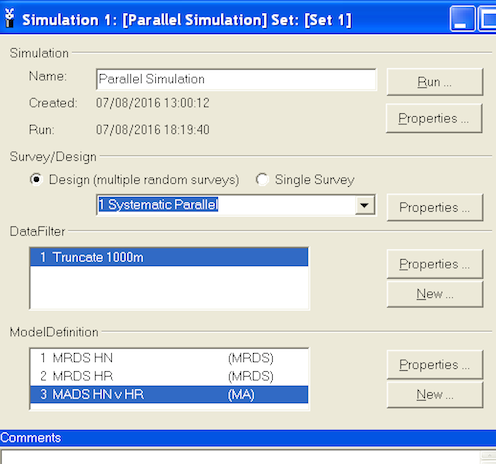
\includegraphics{images/details.png}
\caption{Simulation Details}
\end{figure}

\subsection{Simulation Properties}\label{simulation-properties}

Now click on the Simulation `Properties' button to set the other
simulation properties. The Simulation tab (Figure 4.7) allows us to
specify the geographic layer to use, in this example as we do not have
strata we must select the global study region layer. Here we can also
tell Distance how many times to repeat the simulation and set shapefile
options. It is sensible to run the simulation only once in the first
instance to check the setup is correct. The shapefile options allow us
to tell Distance to save the shapefiles for use in subseqent simulations
using the same design. This can save some processing time. If requested
the shapefiles are stored in the project .dat folder under
`Simulation/Simulation{[}ID{]}/shapefiles'.

\begin{figure}
\centering
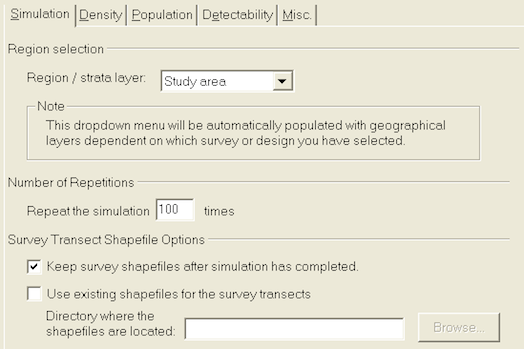
\includegraphics{images/simulation.png}
\caption{Properties Pages: Simulation tab}
\end{figure}

Next we can define our density surface which describes animal
distribution (Figure 4.8). As in exercise 1A we can select a grid
spacing of 1000. Distance has more restricted options than DSsim.
Currently we are only able to specify a constant density surface with
hot/low spots. Note that this density surface is just giving Distance
the relative (rather than absolute) densities.

\begin{figure}
\centering
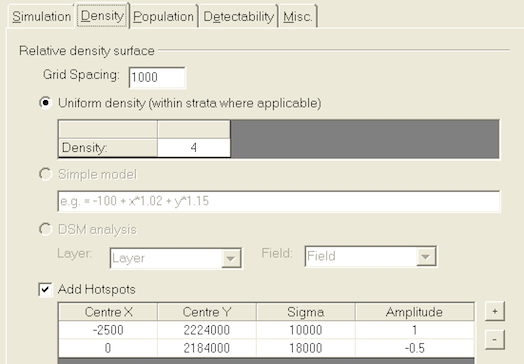
\includegraphics{images/density.png}
\caption{Properties Pages: Density tab}
\end{figure}

\newpage

The Population tab (Figure 4.9) currently only requires that we provide
a population size, in this case 1500.

\begin{figure}
\centering
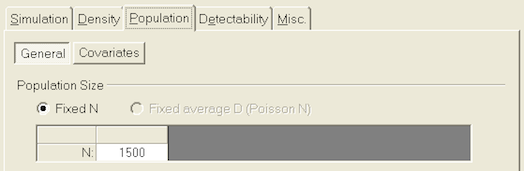
\includegraphics{images/population.png}
\caption{Properties Pages: Population tab}
\end{figure}

Next we describe the detectability of the animals. We will assume a
half-normal detection function with sigma = 500m (Figure 4.10). The
units of the detection function parameters must be the same as those of
the study region and a reminder is provided below the table.

\begin{figure}
\centering
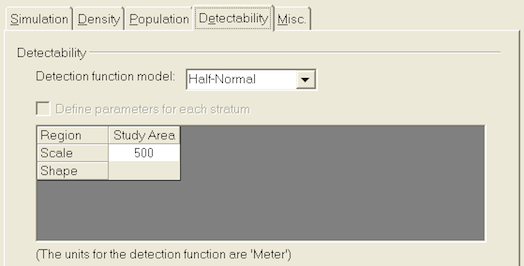
\includegraphics{images/detect.png}
\caption{Properties Pages: Detectability tab}
\end{figure}

Finally we can select some miscelaneous options. These do not affect the
output seen within distance. The option to run the simulation in
parallel can speed things up if running more than a few iterations.
Saving the results from each iteration to file will create csv files
with the individual estimates from each repetition. Saving an example
dataset will create a csv file that is ready to be read into a distance
project for analysis. These files are stored in the project .dat folder
under `Simulation/Simulation{[}ID{]}'.

Further instructions on setting up different simulations options can be
found in the Distance manual.

\subsection{Results}\label{results}

Solutions to this practical can be found in the
DSsimExerciseSolutions.dst project. In this project both the parallel
and zigzag design simulations have been run 100 times.

Note that even though the designs were never initially run to estimate
coverage, when a simulation is run this triggers the design to be run.
Therefore, the design results give the coverage for the actual sets of
transects used in the simulation.

\chapter{Preparing survey data for spatial
analysis}\label{preparing-survey-data-for-spatial-analysis}

\section{Aims}\label{aims}

By the end of this practical, you should feel comfortable:

\begin{itemize}
\tightlist
\item
  Loading data from a geodatabase file into R
\item
  Removing and renaming columns in a \texttt{data.frame}
\item
  Saving data to an \texttt{RData} file
\end{itemize}

Note we can (and should) re-run this file when we update the
\texttt{Analysis.gdb} file to ensure that the data R uses has all of the
covariates we want to use in our analysis.

\section{Preamble}\label{preamble}

Load some useful packages:

\begin{Shaded}
\begin{Highlighting}[]
\KeywordTok{library}\NormalTok{(rgdal)}
\KeywordTok{library}\NormalTok{(knitr)}
\end{Highlighting}
\end{Shaded}

\section{Load and arrange data}\label{load-and-arrange-data}

To fit our spatial models we require three objects:

\begin{enumerate}
\def\labelenumi{\arabic{enumi}.}
\tightlist
\item
  The detection function we fitted previously.
\item
  The segment data (sometimes called effort data). This tells us how
  much effort was expended per segment (in this case how far the boat
  went) and includes the covariates that we want to use to fit our
  model.
\item
  The observation table. This links the observations in the detection
  function object to the segments.
\end{enumerate}

In R we can use the \texttt{rgdal} package to access the geodatabase
files generated by ArcGIS (R can also access shapefiles and rasters).

It can be useful in general to see which ``layers'' are available in the
geodatabase, for that we can use the \texttt{ogrListLayers()} function:

\begin{Shaded}
\begin{Highlighting}[]
\KeywordTok{ogrListLayers}\NormalTok{(}\StringTok{"Analysis.gdb"}\NormalTok{)}
\end{Highlighting}
\end{Shaded}

\begin{verbatim}
##  [1] "EN_Trackline1"     "EN_Trackline2"     "GU_Trackline2"    
##  [4] "GU_Sightings"      "EN_Sightings"      "GU_Trackline"     
##  [7] "Tracklines"        "Tracklines2"       "Segments"         
## [10] "Sightings"         "Segment_Centroids" "Study_Area"       
## [13] "US_Atlantic_EEZ"  
## attr(,"driver")
## [1] "OpenFileGDB"
## attr(,"nlayers")
## [1] 13
\end{verbatim}

\subsection{Segment data}\label{segment-data}

For our analysis the segment data is located in in the
``Segment\_Centroids'' table in the geodatabase. We can import that into
R using the \texttt{readOGR()} function:

\begin{Shaded}
\begin{Highlighting}[]
\NormalTok{segs <-}\StringTok{ }\KeywordTok{readOGR}\NormalTok{(}\StringTok{"Analysis.gdb"}\NormalTok{, }\DataTypeTok{layer=}\StringTok{"Segment_Centroids"}\NormalTok{)}
\end{Highlighting}
\end{Shaded}

\begin{verbatim}
## OGR data source with driver: OpenFileGDB 
## Source: "Analysis.gdb", layer: "Segment_Centroids"
## with 949 features
## It has 10 fields
\end{verbatim}

To verify we have the right data we can plot it. This will give the
locations of each segment:

\begin{Shaded}
\begin{Highlighting}[]
\KeywordTok{plot}\NormalTok{(segs)}
\end{Highlighting}
\end{Shaded}

\begin{figure}
\centering

\includegraphics{_main_files/figure-latex/segs-data-plot-1.pdf}
\caption{\label{fig:segs-data-plot}Segment centroid locations for spearm
whale dataset.}
\end{figure}

A further check would be to use \texttt{head()} to check that the
structure of the data is correct. In particular it's worth checking that
the column names are correct and that the number of rows in the data set
are correct (\texttt{dim()} will give the number of rows and columns).

It can also be useful to check that the columns are the correct data
types. Calling \texttt{str(segs@data)} (or any object loaded using
\texttt{readOGR} appended with \texttt{@data}) will reveal the data
types of each column. In this case we can see that the
\texttt{CenterTime} column has been interpreted as a \texttt{factor}
variable rather than as a date/time. We're not going to use it in our
analysis, so we don't need to worry for now but \texttt{str()} can
reveal potential problems with loaded data.

For a deeper look at the values in the data, \texttt{summary()} will
give summary statistics for each of the covariates as well as the
projection and range of location values (lat/long or in our case
\texttt{x} and \texttt{y}). We can compare these with values in ArcGIS.

We can turn the object into a \texttt{data.frame} (so R can better
understand it) and then check that it looks like it's in the right
format using \texttt{head()}:

\begin{Shaded}
\begin{Highlighting}[]
\NormalTok{segs <-}\StringTok{ }\KeywordTok{as.data.frame}\NormalTok{(segs)}
\KeywordTok{head}\NormalTok{(segs)}
\end{Highlighting}
\end{Shaded}

\begin{verbatim}
##            CenterTime SegmentID   Length  POINT_X  POINT_Y     Depth
## 1 2004/06/24 07:27:04         1 10288.91 214544.0 689074.3  118.5027
## 2 2004/06/24 08:08:04         2 10288.91 222654.3 682781.0  119.4853
## 3 2004/06/24 09:03:18         3 10288.91 230279.9 675473.3  177.2779
## 4 2004/06/24 09:51:27         4 10288.91 239328.9 666646.3  527.9562
## 5 2004/06/24 10:25:39         5 10288.91 246686.5 659459.2  602.6378
## 6 2004/06/24 11:00:22         6 10288.91 254307.0 652547.2 1094.4402
##    DistToCAS      SST          EKE      NPP coords.x1 coords.x2
## 1 14468.1533 15.54390 0.0014442616 1908.129  214544.0  689074.3
## 2 10262.9648 15.88358 0.0014198086 1889.540  222654.3  682781.0
## 3  6900.9829 16.21920 0.0011704842 1842.057  230279.9  675473.3
## 4  1055.4124 16.45468 0.0004101589 1823.942  239328.9  666646.3
## 5  1112.6293 16.62554 0.0002553244 1721.949  246686.5  659459.2
## 6   707.5795 16.83725 0.0006556266 1400.281  254307.0  652547.2
\end{verbatim}

As with the distance data, we need to give the columns of the data
particular names for them to work with \texttt{dsm}:

\begin{Shaded}
\begin{Highlighting}[]
\NormalTok{segs}\OperatorTok{$}\NormalTok{x <-}\StringTok{ }\NormalTok{segs}\OperatorTok{$}\NormalTok{POINT_X}
\NormalTok{segs}\OperatorTok{$}\NormalTok{y <-}\StringTok{ }\NormalTok{segs}\OperatorTok{$}\NormalTok{POINT_Y}
\NormalTok{segs}\OperatorTok{$}\NormalTok{Effort <-}\StringTok{ }\NormalTok{segs}\OperatorTok{$}\NormalTok{Length}
\NormalTok{segs}\OperatorTok{$}\NormalTok{Sample.Label <-}\StringTok{ }\NormalTok{segs}\OperatorTok{$}\NormalTok{SegmentID}
\end{Highlighting}
\end{Shaded}

\subsection{Observation data}\label{observation-data}

The observation data is exactly what we used to fit out detection
function in the previous exercise (though this is not necessarily always
true).

\begin{Shaded}
\begin{Highlighting}[]
\NormalTok{obs <-}\StringTok{ }\KeywordTok{readOGR}\NormalTok{(}\StringTok{"Analysis.gdb"}\NormalTok{, }\DataTypeTok{layer=}\StringTok{"Sightings"}\NormalTok{)}
\end{Highlighting}
\end{Shaded}

\begin{verbatim}
## OGR data source with driver: OpenFileGDB 
## Source: "Analysis.gdb", layer: "Sightings"
## with 137 features
## It has 7 fields
\end{verbatim}

Again we can use a plot to see whether the data looks okay. This time we
only have the locations of the observations:

\begin{Shaded}
\begin{Highlighting}[]
\KeywordTok{plot}\NormalTok{(obs)}
\end{Highlighting}
\end{Shaded}

\begin{figure}
\centering
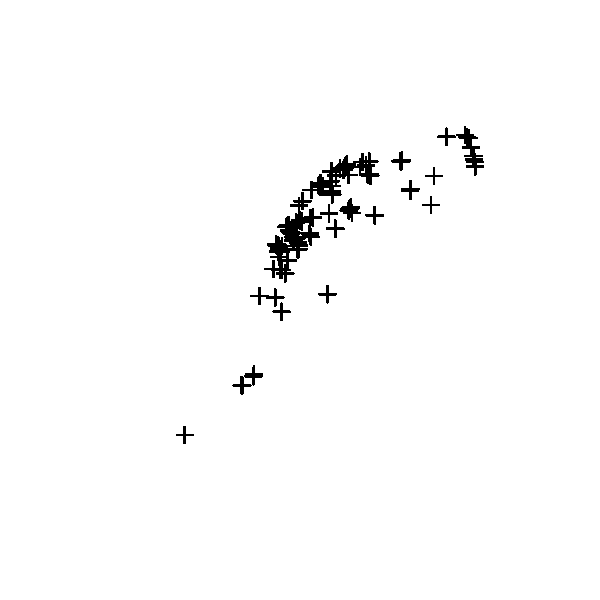
\includegraphics{_main_files/figure-latex/obs-data-plot-1.pdf}
\caption{\label{fig:obs-data-plot}Sighting locations for spearm whale
dataset.}
\end{figure}

Again, converting the object to be a \texttt{data.frame} and checking
it's format using \texttt{head()}:

\begin{Shaded}
\begin{Highlighting}[]
\NormalTok{obs <-}\StringTok{ }\KeywordTok{as.data.frame}\NormalTok{(obs)}
\KeywordTok{head}\NormalTok{(obs)}
\end{Highlighting}
\end{Shaded}

\begin{verbatim}
##    Survey GroupSize SeaState  Distance        SightingTime SegmentID
## 1 en04395         2      3.0  246.0173 2004/06/28 10:22:21        48
## 2 en04395         2      2.5 1632.3934 2004/06/28 13:18:14        50
## 3 en04395         1      3.0 2368.9941 2004/06/28 14:13:34        51
## 4 en04395         1      3.5  244.6977 2004/06/28 15:06:01        52
## 5 en04395         1      4.0 2081.3468 2004/06/29 10:48:31        56
## 6 en04395         1      2.4 1149.2632 2004/06/29 14:35:33        59
##   SightingID coords.x1 coords.x2
## 1          1   -65.636    39.576
## 2          2   -65.648    39.746
## 3          3   -65.692    39.843
## 4          4   -65.717    39.967
## 5          5   -65.820    40.279
## 6          6   -65.938    40.612
\end{verbatim}

Finally, we need to rename some of the columns:

\begin{Shaded}
\begin{Highlighting}[]
\NormalTok{obs}\OperatorTok{$}\NormalTok{distance <-}\StringTok{ }\NormalTok{obs}\OperatorTok{$}\NormalTok{Distance}
\NormalTok{obs}\OperatorTok{$}\NormalTok{object <-}\StringTok{ }\NormalTok{obs}\OperatorTok{$}\NormalTok{SightingID}
\NormalTok{obs}\OperatorTok{$}\NormalTok{Sample.Label <-}\StringTok{ }\NormalTok{obs}\OperatorTok{$}\NormalTok{SegmentID}
\NormalTok{obs}\OperatorTok{$}\NormalTok{size <-}\StringTok{ }\NormalTok{obs}\OperatorTok{$}\NormalTok{GroupSize}
\end{Highlighting}
\end{Shaded}

\section{Save the data}\label{save-the-data}

We can now save the \texttt{data.frame}s that we've created into an
\texttt{RData} file so we can use them later.

\begin{Shaded}
\begin{Highlighting}[]
\KeywordTok{save}\NormalTok{(segs, obs, }\DataTypeTok{file=}\StringTok{"sperm-data.RData"}\NormalTok{)}
\end{Highlighting}
\end{Shaded}

\chapter{Detection function fitting}\label{detection-function-fitting}

\section{Aims}\label{aims-1}

By the end of this practical you should feel confident doing the
following:

\begin{itemize}
\tightlist
\item
  Loading data from ArcGIS \texttt{.gdb} files
\item
  Working on a \texttt{data.frame} in R to get it into the correct
  format for \texttt{Distance}
\item
  Fitting a detection function using \texttt{ds()}
\item
  Checking detection functions
\item
  Making at goodness of fit plots
\item
  Selecting models using AIC
\item
  Estimating abundance (using R and maths!)
\end{itemize}

\section{Preamble}\label{preamble-1}

First need to load the requisite R libraries

\begin{Shaded}
\begin{Highlighting}[]
\KeywordTok{library}\NormalTok{(rgdal)}
\KeywordTok{library}\NormalTok{(ggplot2)}
\KeywordTok{library}\NormalTok{(Distance)}
\end{Highlighting}
\end{Shaded}

\begin{verbatim}
## 
## Attaching package: 'Distance'
\end{verbatim}

\begin{verbatim}
## The following object is masked from 'package:mrds':
## 
##     create.bins
\end{verbatim}

\begin{Shaded}
\begin{Highlighting}[]
\KeywordTok{library}\NormalTok{(knitr)}
\KeywordTok{library}\NormalTok{(kableExtra)}
\end{Highlighting}
\end{Shaded}

\section{Load the data}\label{load-the-data}

The observations are located in a ``geodatabase'' we created in Arc. We
want to pull out the ``Sightings'' table (called a ``layer'') and make
it into a \texttt{data.frame} (so it's easier for R to manipulate).

\begin{Shaded}
\begin{Highlighting}[]
\NormalTok{distdata <-}\StringTok{ }\KeywordTok{readOGR}\NormalTok{(}\StringTok{"Analysis.gdb"}\NormalTok{, }\DataTypeTok{layer=}\StringTok{"Sightings"}\NormalTok{)}
\end{Highlighting}
\end{Shaded}

\begin{verbatim}
## OGR data source with driver: OpenFileGDB 
## Source: "Analysis.gdb", layer: "Sightings"
## with 137 features
## It has 7 fields
\end{verbatim}

\begin{Shaded}
\begin{Highlighting}[]
\NormalTok{distdata <-}\StringTok{ }\KeywordTok{as.data.frame}\NormalTok{(distdata)}
\end{Highlighting}
\end{Shaded}

We can check it has the correct format using \texttt{head}:

\begin{Shaded}
\begin{Highlighting}[]
\KeywordTok{head}\NormalTok{(distdata)}
\end{Highlighting}
\end{Shaded}

\begin{verbatim}
##    Survey GroupSize SeaState  Distance        SightingTime SegmentID
## 1 en04395         2      3.0  246.0173 2004/06/28 10:22:21        48
## 2 en04395         2      2.5 1632.3934 2004/06/28 13:18:14        50
## 3 en04395         1      3.0 2368.9941 2004/06/28 14:13:34        51
## 4 en04395         1      3.5  244.6977 2004/06/28 15:06:01        52
## 5 en04395         1      4.0 2081.3468 2004/06/29 10:48:31        56
## 6 en04395         1      2.4 1149.2632 2004/06/29 14:35:33        59
##   SightingID coords.x1 coords.x2
## 1          1   -65.636    39.576
## 2          2   -65.648    39.746
## 3          3   -65.692    39.843
## 4          4   -65.717    39.967
## 5          5   -65.820    40.279
## 6          6   -65.938    40.612
\end{verbatim}

The \texttt{Distance} package expects certain column names to be used.
Renaming is much easier to do in R than ArcGIS, so we do it here.

\begin{Shaded}
\begin{Highlighting}[]
\NormalTok{distdata}\OperatorTok{$}\NormalTok{distance <-}\StringTok{ }\NormalTok{distdata}\OperatorTok{$}\NormalTok{Distance}
\NormalTok{distdata}\OperatorTok{$}\NormalTok{object <-}\StringTok{ }\NormalTok{distdata}\OperatorTok{$}\NormalTok{SightingID}
\NormalTok{distdata}\OperatorTok{$}\NormalTok{size <-}\StringTok{ }\NormalTok{distdata}\OperatorTok{$}\NormalTok{GroupSize}
\end{Highlighting}
\end{Shaded}

Let's see what we did:

\begin{Shaded}
\begin{Highlighting}[]
\KeywordTok{head}\NormalTok{(distdata)}
\end{Highlighting}
\end{Shaded}

\begin{verbatim}
##    Survey GroupSize SeaState  Distance        SightingTime SegmentID
## 1 en04395         2      3.0  246.0173 2004/06/28 10:22:21        48
## 2 en04395         2      2.5 1632.3934 2004/06/28 13:18:14        50
## 3 en04395         1      3.0 2368.9941 2004/06/28 14:13:34        51
## 4 en04395         1      3.5  244.6977 2004/06/28 15:06:01        52
## 5 en04395         1      4.0 2081.3468 2004/06/29 10:48:31        56
## 6 en04395         1      2.4 1149.2632 2004/06/29 14:35:33        59
##   SightingID coords.x1 coords.x2  distance object size
## 1          1   -65.636    39.576  246.0173      1    2
## 2          2   -65.648    39.746 1632.3934      2    2
## 3          3   -65.692    39.843 2368.9941      3    1
## 4          4   -65.717    39.967  244.6977      4    1
## 5          5   -65.820    40.279 2081.3468      5    1
## 6          6   -65.938    40.612 1149.2632      6    1
\end{verbatim}

We now have four ``extra'' columns.

\section{Exploratory analysis}\label{exploratory-analysis}

Before setting off fitting detection functions, let's look at the
relationship of various variables in the data.

\emph{Don't worry too much about understanding the code that generates
these plots at the moment.}

\subsection{Distances}\label{distances}

Obviously, the most important covariate in a distance sampling analysis
is distance itself. We can plot a histogram of the distances to check
that (1) we imported the data correctly and (2) it conforms to the usual
shape for line transect data.

\begin{Shaded}
\begin{Highlighting}[]
\KeywordTok{hist}\NormalTok{(distdata}\OperatorTok{$}\NormalTok{distance, }\DataTypeTok{xlab=}\StringTok{"Distance (m)"}\NormalTok{, }\DataTypeTok{main=}\StringTok{"Distance to sperm whale observations"}\NormalTok{)}
\end{Highlighting}
\end{Shaded}

\begin{figure}
\centering
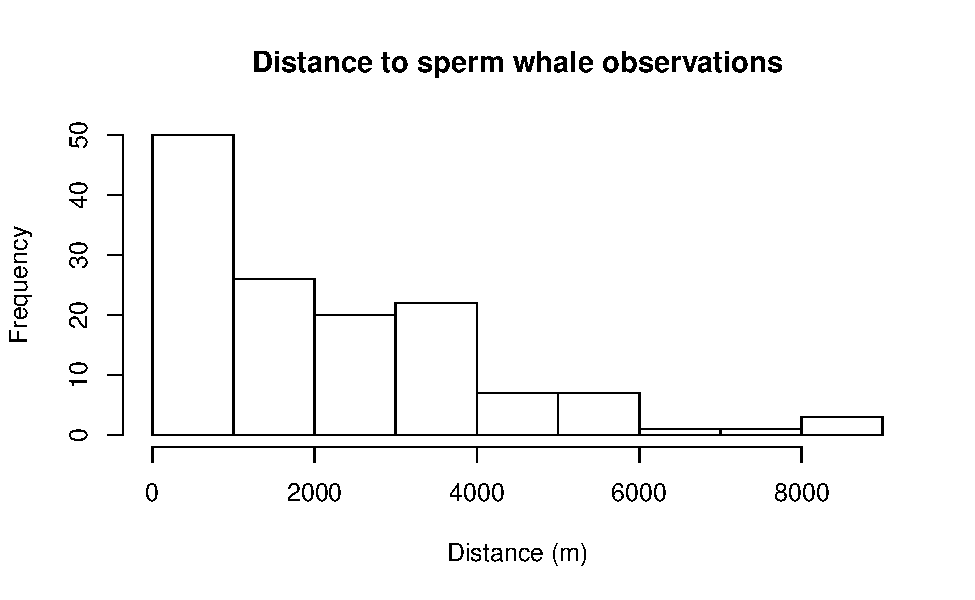
\includegraphics{_main_files/figure-latex/eda-dist-1.pdf}
\caption{\label{fig:eda-dist}Distribution of observed perpendicular
detection distances.}
\end{figure}

\subsection{Size and distance}\label{size-and-distance}

We might expect that there will be a relationship between the distance
at which we see animals and the size of the groups observed (larger
groups are easier to see at larger distances), so let's plot that to
help us visualise the relationship.

\begin{Shaded}
\begin{Highlighting}[]
\CommentTok{# plot of size versus distance and sea state vs distance, linear model and LOESS smoother overlay}

\CommentTok{# put the data into a simple format, only selecting what we need}
\NormalTok{distplot <-}\StringTok{ }\NormalTok{distdata[,}\KeywordTok{c}\NormalTok{(}\StringTok{"distance"}\NormalTok{,}\StringTok{"size"}\NormalTok{,}\StringTok{"SeaState"}\NormalTok{)]}
\KeywordTok{names}\NormalTok{(distplot) <-}\StringTok{ }\KeywordTok{c}\NormalTok{(}\StringTok{"Distance"}\NormalTok{, }\StringTok{"Size"}\NormalTok{, }\StringTok{"Beaufort"}\NormalTok{)}
\KeywordTok{library}\NormalTok{(reshape2)}
\CommentTok{# "melt" the data to have only three columns (try head(distplot))}
\NormalTok{distplot <-}\StringTok{ }\KeywordTok{melt}\NormalTok{(distplot, }\DataTypeTok{id.vars=}\StringTok{"Distance"}\NormalTok{, }\DataTypeTok{value.name=}\StringTok{"covariate"}\NormalTok{)}

\CommentTok{# make the plot}
\NormalTok{p <-}\StringTok{ }\KeywordTok{ggplot}\NormalTok{(distplot, }\KeywordTok{aes}\NormalTok{(}\DataTypeTok{x=}\NormalTok{covariate, }\DataTypeTok{y=}\NormalTok{Distance)) }\OperatorTok{+}
\StringTok{      }\KeywordTok{geom_point}\NormalTok{() }\OperatorTok{+}
\StringTok{      }\KeywordTok{facet_wrap}\NormalTok{(}\OperatorTok{~}\NormalTok{variable, }\DataTypeTok{scale=}\StringTok{"free"}\NormalTok{) }\OperatorTok{+}
\StringTok{      }\KeywordTok{geom_smooth}\NormalTok{(}\DataTypeTok{method=}\StringTok{"loess"}\NormalTok{, }\DataTypeTok{se=}\OtherTok{FALSE}\NormalTok{) }\OperatorTok{+}
\StringTok{      }\KeywordTok{geom_smooth}\NormalTok{(}\DataTypeTok{method=}\StringTok{"lm"}\NormalTok{, }\DataTypeTok{se=}\OtherTok{FALSE}\NormalTok{) }\OperatorTok{+}
\StringTok{      }\KeywordTok{labs}\NormalTok{(}\DataTypeTok{x=}\StringTok{"Covariate value"}\NormalTok{, }\DataTypeTok{y=}\StringTok{"Distance (m)"}\NormalTok{)}
\KeywordTok{print}\NormalTok{(p)}
\end{Highlighting}
\end{Shaded}

\begin{figure}
\centering
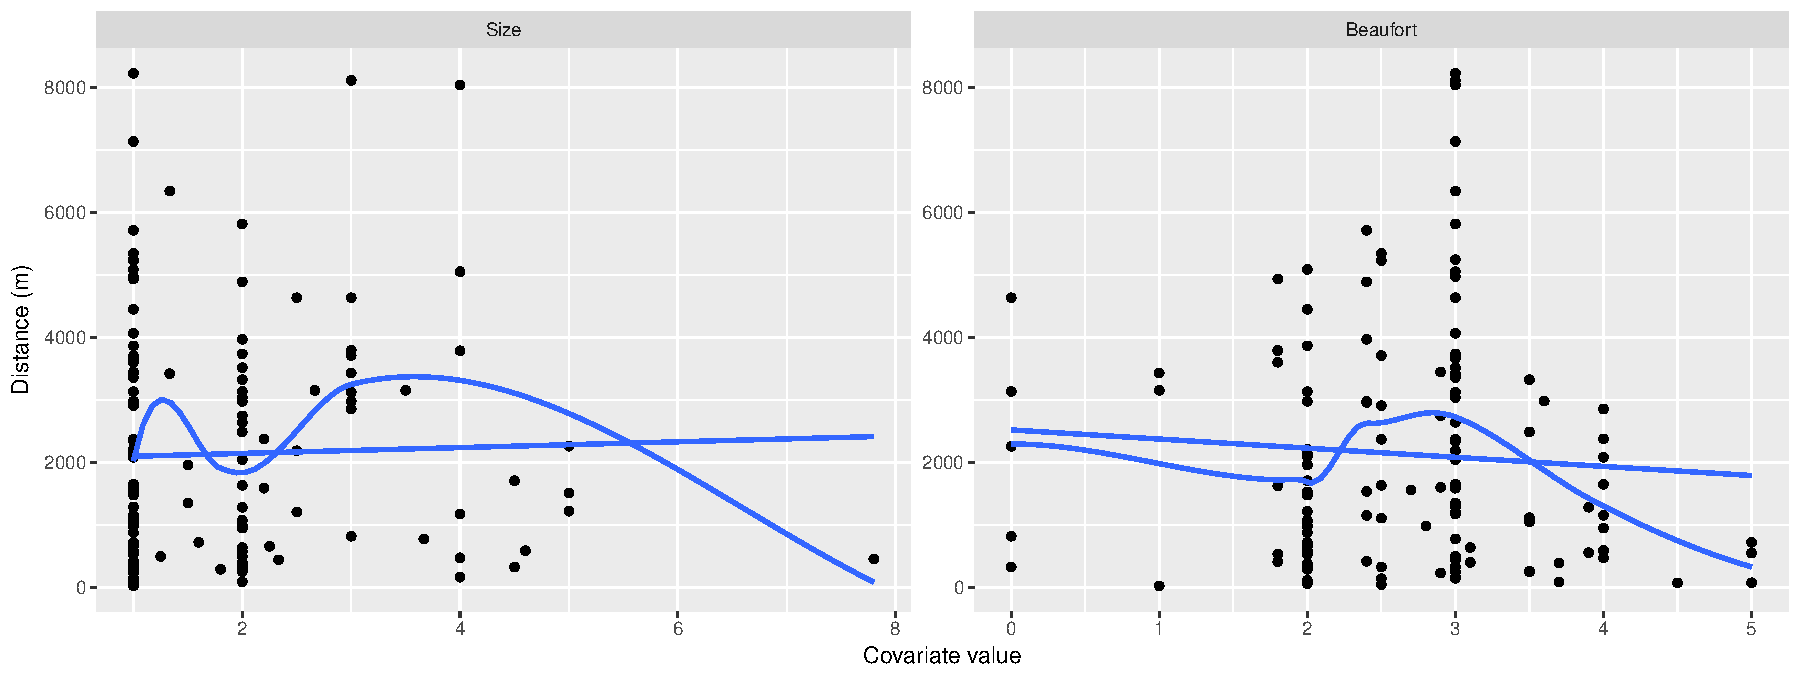
\includegraphics{_main_files/figure-latex/eda-covars-1.pdf}
\caption{\label{fig:eda-covars}Effect of group size upon detection
distances.}
\end{figure}

\subsection{Distance and sea state}\label{distance-and-sea-state}

We might also expect that increasing sea state would result in a drop in
observations. We can plot histograms of distance for each sea state
level (making the sea state take only values 0,1,2,4,5 for this).

\begin{Shaded}
\begin{Highlighting}[]
\NormalTok{distdata}\OperatorTok{$}\NormalTok{SeaStateCut <-}\StringTok{ }\KeywordTok{cut}\NormalTok{(distdata}\OperatorTok{$}\NormalTok{SeaState,}\KeywordTok{seq}\NormalTok{(}\DecValTok{0}\NormalTok{,}\DecValTok{5}\NormalTok{,}\DataTypeTok{by=}\DecValTok{1}\NormalTok{), }\DataTypeTok{include.lowest=}\OtherTok{TRUE}\NormalTok{)}
\NormalTok{p <-}\StringTok{ }\KeywordTok{ggplot}\NormalTok{(distdata) }\OperatorTok{+}
\StringTok{      }\KeywordTok{geom_histogram}\NormalTok{(}\KeywordTok{aes}\NormalTok{(distance)) }\OperatorTok{+}
\StringTok{      }\KeywordTok{facet_wrap}\NormalTok{(}\OperatorTok{~}\NormalTok{SeaStateCut) }\OperatorTok{+}
\StringTok{      }\KeywordTok{labs}\NormalTok{(}\DataTypeTok{x=}\StringTok{"Distance (m)"}\NormalTok{, }\DataTypeTok{y=}\StringTok{"Count"}\NormalTok{)}
\KeywordTok{print}\NormalTok{(p)}
\end{Highlighting}
\end{Shaded}

\begin{verbatim}
## `stat_bin()` using `bins = 30`. Pick better value with `binwidth`.
\end{verbatim}

\begin{figure}
\centering
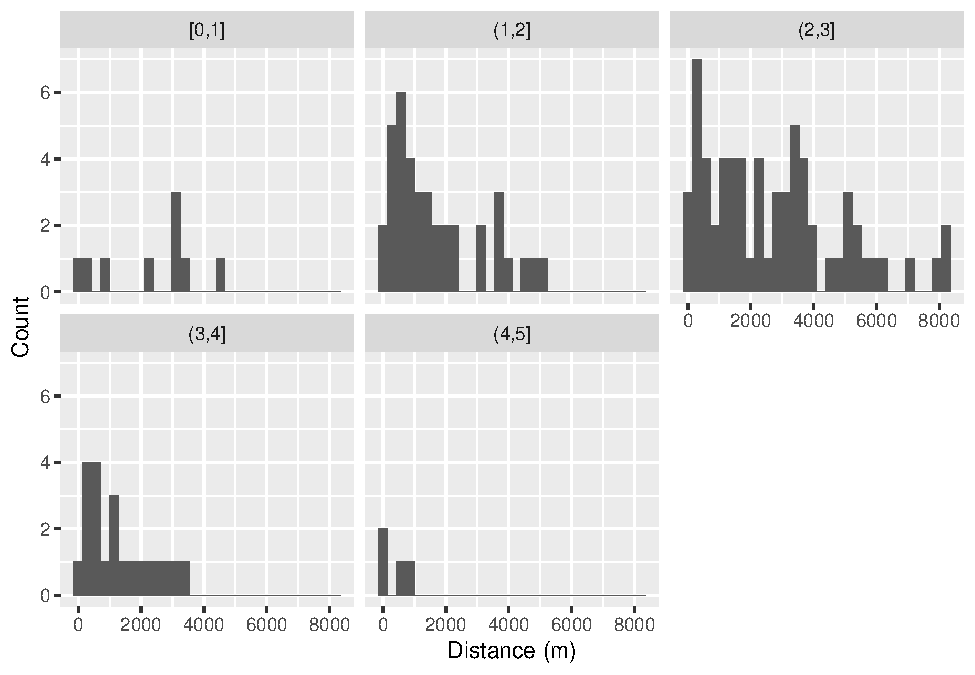
\includegraphics{_main_files/figure-latex/eda-dist-facet-seastate-1.pdf}
\caption{\label{fig:eda-dist-facet-seastate}Effect of sea state upon
detection distances.}
\end{figure}

\subsection{Survey effect}\label{survey-effect}

Given we are including data from two different surveys we can also
investigate the relationship between survey and distances observed.

\begin{Shaded}
\begin{Highlighting}[]
\NormalTok{p <-}\StringTok{ }\KeywordTok{ggplot}\NormalTok{(distdata) }\OperatorTok{+}
\StringTok{      }\KeywordTok{geom_histogram}\NormalTok{(}\KeywordTok{aes}\NormalTok{(distance)) }\OperatorTok{+}
\StringTok{      }\KeywordTok{facet_wrap}\NormalTok{(}\OperatorTok{~}\NormalTok{Survey) }\OperatorTok{+}
\StringTok{      }\KeywordTok{labs}\NormalTok{(}\DataTypeTok{x=}\StringTok{"Distance (m)"}\NormalTok{, }\DataTypeTok{y=}\StringTok{"Count"}\NormalTok{)}
\KeywordTok{print}\NormalTok{(p)}
\end{Highlighting}
\end{Shaded}

\begin{verbatim}
## `stat_bin()` using `bins = 30`. Pick better value with `binwidth`.
\end{verbatim}

\begin{figure}
\centering
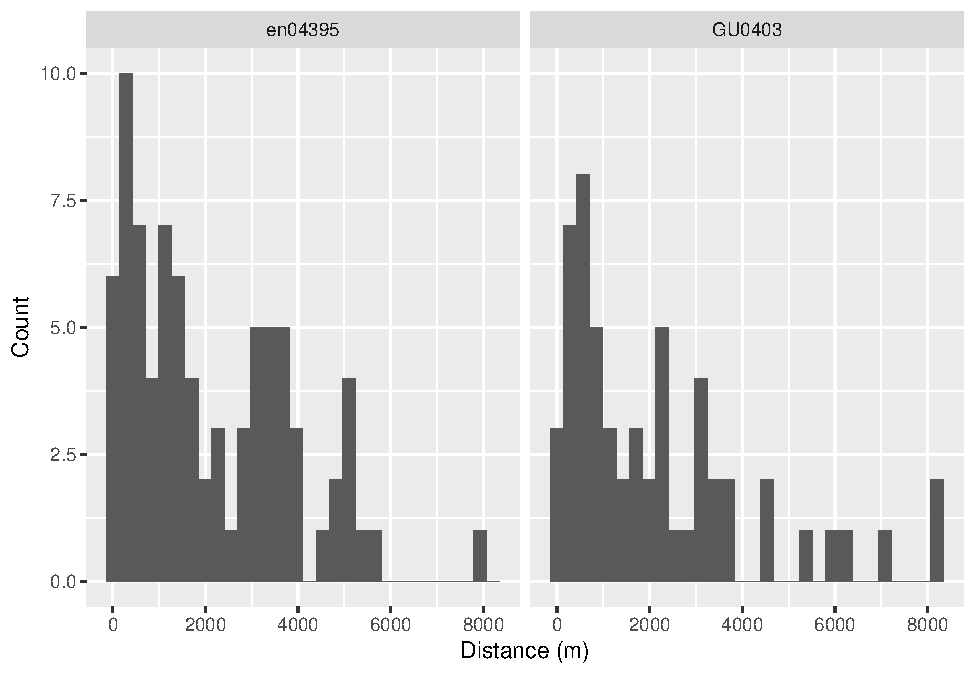
\includegraphics{_main_files/figure-latex/eda-dist-facet-survey-1.pdf}
\caption{\label{fig:eda-dist-facet-survey}Effect of survey upon detection
distances.}
\end{figure}

\section{Fitting detection functions}\label{fitting-detection-functions}

It's now time to fit some detection function models. We'll use the
\texttt{ds()} function from the \texttt{Distance} package to fit the
detection function. You can access the help file for the \texttt{ds()}
function by typing \texttt{?ds} -- this will give you information about
what the different arguments to the function are and what they do.

We can fit a very simple model with the following code:

\begin{Shaded}
\begin{Highlighting}[]
\NormalTok{df_hn <-}\StringTok{ }\KeywordTok{ds}\NormalTok{(}\DataTypeTok{data=}\NormalTok{distdata, }\DataTypeTok{truncation=}\DecValTok{6000}\NormalTok{, }\DataTypeTok{key=}\StringTok{"hn"}\NormalTok{, }\DataTypeTok{adjustment=}\OtherTok{NULL}\NormalTok{)}
\end{Highlighting}
\end{Shaded}

\begin{verbatim}
## Fitting half-normal key function
\end{verbatim}

\begin{verbatim}
## Key only model: not constraining for monotonicity.
\end{verbatim}

\begin{verbatim}
## AIC= 2252.06
\end{verbatim}

\begin{verbatim}
## No survey area information supplied, only estimating detection function.
\end{verbatim}

Let's dissect the call and see what each argument means:

\begin{itemize}
\tightlist
\item
  \texttt{data=distdata}: the data to use to fit the model, as we
  prepared above.
\item
  \texttt{truncation=6000}: set the truncation distance. Here,
  observations at distances greater than 6000m will be discarded before
  fitting the detection function.
\item
  \texttt{key="hn"}: the key function to use for the detection function,
  in this case half-normal (\texttt{?ds} lists the other options).
\item
  \texttt{adjustment=NULL}: adjustment term series to fit. \texttt{NULL}
  here means that no adjustments should be fitted (again \texttt{?ds}
  lists all options).
\end{itemize}

Other useful arguments for this practical are:

\begin{itemize}
\tightlist
\item
  \texttt{formula=}: gives the formula to use for the scale parameter.
  By default it takes the value \texttt{\textasciitilde{}1}, meaning the
  scale parameter is constant and not a function of covariates.
\item
  \texttt{order=}: specifies the ``order'' of the adjustments to be
  used. This is a number (or vector of numbers) specifying the order of
  the terms. For example \texttt{order=2} fits order 2 adjustments,
  \texttt{order=c(2,3)} will fit a model with order 2 and 3 adjustments
  (mathematically, it only makes sense to include order 3 with order 2).
  By default the value is \texttt{NULL} which has \texttt{ds()} select
  the number of adjustments by AIC.
\end{itemize}

\subsection{Summaries}\label{summaries}

We can look at the summary of the fitted detection function using the
\texttt{summary()} function:

\begin{Shaded}
\begin{Highlighting}[]
\KeywordTok{summary}\NormalTok{(df_hn)}
\end{Highlighting}
\end{Shaded}

\begin{verbatim}
## 
## Summary for distance analysis 
## Number of observations :  132 
## Distance range         :  0  -  6000 
## 
## Model : Half-normal key function 
## AIC   : 2252.06 
## 
## Detection function parameters
## Scale coefficient(s):  
##             estimate         se
## (Intercept) 7.900732 0.07884776
## 
##                        Estimate          SE         CV
## Average p             0.5490484  0.03662569 0.06670757
## N in covered region 240.4159539 21.32287581 0.08869160
\end{verbatim}

\subsection{Goodness of fit}\label{goodness-of-fit}

Goodness of fit quantile-quantile plot and test results can be accessed
using the \texttt{ddf.gof()} function:

\begin{Shaded}
\begin{Highlighting}[]
\KeywordTok{ddf.gof}\NormalTok{(df_hn}\OperatorTok{$}\NormalTok{ddf)}
\end{Highlighting}
\end{Shaded}

\begin{figure}
\centering
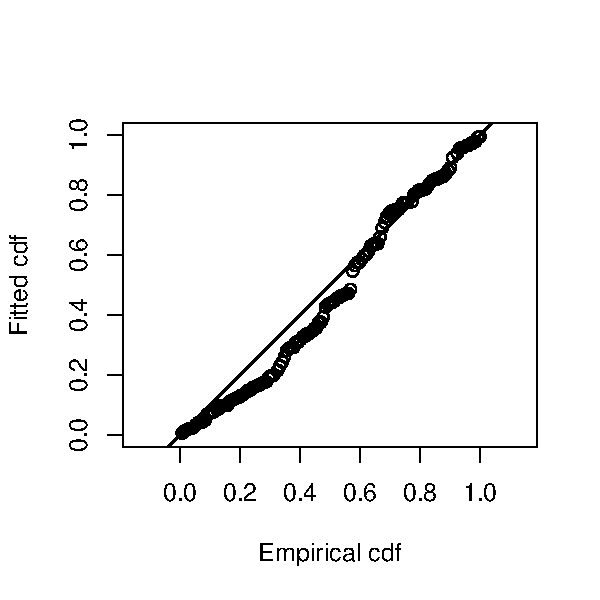
\includegraphics{_main_files/figure-latex/simple-gof-1.pdf}
\caption{\label{fig:simple-gof}Goodness of fit QQ plot of half-normal
detection function.}
\end{figure}

\begin{verbatim}
## 
## Goodness of fit results for ddf object
## 
## Chi-square tests
##             [0,545] (545,1.09e+03] (1.09e+03,1.64e+03] (1.64e+03,2.18e+03]
## Observed  33.000000    20.00000000        19.000000000            8.000000
## Expected  21.708156    20.84245788        19.213254554           17.005089
## Chisquare  5.873634     0.03405238         0.002366986            4.768669
##           (2.18e+03,2.73e+03] (2.73e+03,3.27e+03] (3.27e+03,3.82e+03]
## Observed             9.000000          13.0000000           14.000000
## Expected            14.450499          11.7899695            9.235669
## Chisquare            2.055842           0.1241881            2.457737
##           (3.82e+03,4.36e+03] (4.36e+03,4.91e+03] (4.91e+03,5.45e+03]
## Observed             3.000000           4.0000000            7.000000
## Expected             6.946241           5.0159948            3.477683
## Chisquare            2.241906           0.2057908            3.567525
##           (5.45e+03,6e+03]     Total
## Observed        2.00000000 132.00000
## Expected        2.31498601 132.00000
## Chisquare       0.04285822  21.37457
## 
## P = 0.011087 with 9 degrees of freedom
## 
## Distance sampling Kolmogorov-Smirnov test
## Test statistic =  0.11192  P =  0.073241 
## 
## Distance sampling Cramer-von Mises test (unweighted)
## Test statistic =  0.39618  P =  0.073947
\end{verbatim}

Note two things here: 1. We use the \texttt{\$ddf} element of the
detection function object 2. We're ignoring the \(\chi^2\) test results,
as they rely on binning the distances to calculate test statistics where
as Cramer-von Mises and Kolmogorov-Smirnov tests do not.

\subsection{Plotting}\label{plotting}

We can plot the models simply using the \texttt{plot()} function:

\begin{Shaded}
\begin{Highlighting}[]
\KeywordTok{plot}\NormalTok{(df_hn)}
\end{Highlighting}
\end{Shaded}

\begin{figure}
\centering
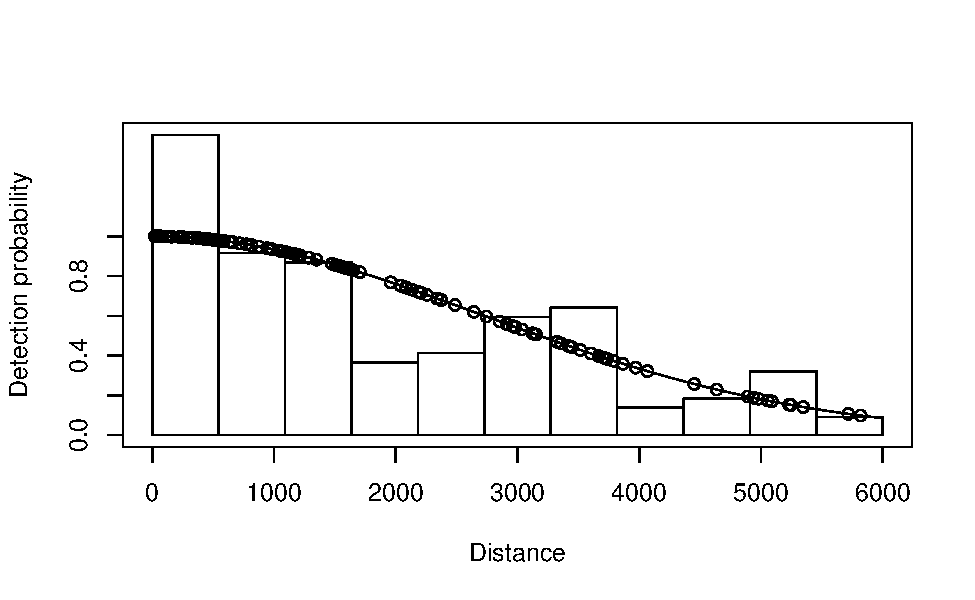
\includegraphics{_main_files/figure-latex/simple-plot-1.pdf}
\caption{\label{fig:simple-plot}Half-normal detection function.}
\end{figure}

The dots on the plot indicate the distances where observations are. We
can remove them (particularly useful for a model without covariates)
using the additional argument \texttt{showpoints=FALSE} (try this out!).

\section{Now you try\ldots{}}\label{now-you-try}

Now try fitting a few models and comparing them using AIC. Don't try to
fit all possible models, just try a selection (say, a hazard-rate, a
model with adjustments and a couple with different covariates). You can
also try out changing the truncation distance.

Here's an example to work from. Some tips before you start:

\begin{itemize}
\tightlist
\item
  You can include as many lines as you like in a given chunk (though you
  may find it more manageable to separate them up, remembering each time
  to give the chunk a unique name).
\item
  You can run the current line of code in RStudio by hitting
  \texttt{Control+Enter} (on Windows/Linux; \texttt{Command+Enter} on
  Mac).
\item
  Giving your models informative names will help later on! Here I'm
  using \texttt{df\_} to indicate that this is a detection function,
  then shortened forms of the model form and covariates, separated by
  underscores, but use what makes sense to you (and future you!).
\end{itemize}

\begin{Shaded}
\begin{Highlighting}[]
\NormalTok{df_hr_ss_size <-}\StringTok{ }\KeywordTok{ds}\NormalTok{(distdata, }\DataTypeTok{truncation=}\DecValTok{6000}\NormalTok{, }\DataTypeTok{adjustment=}\OtherTok{NULL}\NormalTok{, }
                    \DataTypeTok{key=}\StringTok{"hr"}\NormalTok{, }\DataTypeTok{formula=}\OperatorTok{~}\NormalTok{SeaState}\OperatorTok{+}\NormalTok{size)}
\end{Highlighting}
\end{Shaded}

\begin{verbatim}
## Fitting hazard-rate key function
\end{verbatim}

\begin{verbatim}
## AIC= 2249.327
\end{verbatim}

\begin{verbatim}
## No survey area information supplied, only estimating detection function.
\end{verbatim}

Once you have the hang of writing models and looking at the differences
between them, you should move onto the next section.

\section{Model selection}\label{model-selection}

Looking at the models individually can be a bit unwieldy -- it's nicer
to put that data into a table and sort the table by the relevant
statistic. The function \texttt{summarize\_ds\_models()} in the
\texttt{Distance} package performs this task for us.

The code below will make a results table with relevant statistics for
model selection in it. The \texttt{summarize\_ds\_models()} function
takes a series of object names as its first argument. We can do that
with the two models that I fitted like so:

\begin{Shaded}
\begin{Highlighting}[]
\NormalTok{model_table <-}\StringTok{ }\KeywordTok{summarize_ds_models}\NormalTok{(df_hn, df_hr_ss_size)}
\KeywordTok{kable}\NormalTok{(model_table, }\DataTypeTok{digits=}\DecValTok{3}\NormalTok{, }\DataTypeTok{format=}\StringTok{"latex"}\NormalTok{, }\DataTypeTok{booktabs=}\OtherTok{TRUE}\NormalTok{, }\DataTypeTok{row.names =} \OtherTok{FALSE}\NormalTok{, }\DataTypeTok{escape=}\OtherTok{FALSE}\NormalTok{,}
      \DataTypeTok{caption =} \StringTok{"Comparison of half normal and hazard rate with sea state and group size."}\NormalTok{) }\OperatorTok
\StringTok{  }\KeywordTok{kable_styling}\NormalTok{(}\DataTypeTok{latex_options=}\StringTok{"scale_down"}\NormalTok{)}
\end{Highlighting}
\end{Shaded}

\begin{table}

\caption{\label{tab:df-results}Comparison of half normal and hazard rate with sea state and group size.}
\centering
\resizebox{\linewidth}{!}{\begin{tabular}[t]{lllrrrr}
\toprule
Model & Key function & Formula & C-vM p-value & $\hat{P_a}$ & se($\hat{P_a}$) & $\Delta$AIC\\
\midrule
\texttt{df\char`_hr\char`_ss\char`_size} & Hazard-rate & ~SeaState + size & 0.880 & 0.355 & 0.074 & 0.000\\
\texttt{df\char`_hn} & Half-normal & ~1 & 0.074 & 0.549 & 0.037 & 2.733\\
\bottomrule
\end{tabular}}
\end{table}

(You can add the models you fitted above into this list.)

\subsubsection{A further note about model selection for the sperm whale
data}\label{a-further-note-about-model-selection-for-the-sperm-whale-data}

Note that there is a considerable spike in our distance data. This may
be down to observers guarding the trackline (spending too much time
searching near zero distance). It's therefore possible that the
hazard-rate model is overfitting to this peak. So we'd like to
investigate results from the half-normal model too and see what the
effects are on the final spatial models.

\subsection{Estimating abundance}\label{estimating-abundance}

Just for fun, let's estimate abundance from these models using a
Horvtiz-Thompson-type estimator.

We know the Horvitz-Thompson estimator has the following form: \[
\hat{N} = \frac{A}{a} \sum_{i=1}^n \frac{s_i}{p_i}
\] we can calculate each part of this equation in R:

\begin{itemize}
\tightlist
\item
  \texttt{A} is the total area of the region we want to estimate
  abundance for. This was \(A=5.285e+11 m^2\).
\item
  \texttt{a} is the total area we surveyed. We know that the total
  transect length was 9,498,474m and the truncation distance. Knowing
  that \(a=2wL\) we can calculate \(a\).
\item
  \(s_i\) are the group sizes, they are stored in
  \texttt{df\_hn\$ddf\$data\$size}.
\item
  \(p_i\) are the probabilities of detection, we can obtain them using
  \texttt{predict(df\_hn\$ddf)\$fitted}.
\end{itemize}

We know that in general operations are vectorised in R, so calculating
\texttt{c(1,\ 2,\ 3)/c(4,\ 5,\ 6)} will give \texttt{c(1/4,\ 2/5,\ 3/6)}
so we can just divide the results of getting the \(s_i\) and \(p_i\)
values and then use the \texttt{sum()} function to sum them up.

Try out estimating abundance using the formula below using both
\texttt{df\_hn} and your favourite model from above:

Note that in the solutions to this exercise (posted on the course
website) I show how to use the function \texttt{dht()} to estimate
abundance (and uncertainty) for a detection function analysis. This
involves some more complex data manipulation steps, so we've left it out
here in favour of getting to grips with the mathematics.

\subsubsection{Accounting for perception
bias}\label{accounting-for-perception-bias}

It's common, especially in marine surveys, for animals at zero distance
to be missed by observers. There are several ways to deal with this
issue. For now, we are just going to use a very simply constant
correction factor to inflate the abundance.

From Palka (\protect\hyperlink{ref-Palka2006}{2006}), we think that
observations on the track line were such that \(g(0)=0.46\), we can
apply that correction to our abundance estimate (in a very primitive
way):

This kind of correction works fine when we have a single number to
adjust by, in general we'd like to model the perception bias using
``mark-recapture distance sampling'' techniques.

\subsection{Save model objects}\label{save-model-objects}

Save your top few models in an \texttt{RData} file, so we can load them
up later on. We'll also save the distance data we used to fit out
models.

\begin{Shaded}
\begin{Highlighting}[]
\KeywordTok{save}\NormalTok{(df_hn, df_hr_ss_size, }\CommentTok{# add you models here, followed by commas!}
\NormalTok{     distdata,}
     \DataTypeTok{file=}\StringTok{"df-models.RData"}\NormalTok{)}
\end{Highlighting}
\end{Shaded}

You can check it worked by using the \texttt{load()} function to recover
the models.

\chapter{Simple density surface
models}\label{simple-density-surface-models}

\section{Aims}\label{aims-2}

By the end of this practical, you should feel comfortable:

\begin{itemize}
\tightlist
\item
  Fitting a density surface model using \texttt{dsm()}
\item
  Understanding what the objects that go into a \texttt{dsm()} call
\item
  Understanding the role of the response in the \texttt{formula=}
  argument
\item
  Understanding the output of \texttt{summary()} when called on a
  \texttt{dsm} object
\item
  Increasing the \texttt{k} parameter of smooth terms to increase their
  flexibility
\item
  Interpreting \texttt{gam.check} and \texttt{rqgam.check} plots and
  diagnostic output
\end{itemize}

The example code below uses the \texttt{df\_hn} detection function in
the density surface models. You can substitute this for your own best
model as you go, or copy and paste the code at the end and see what
results you get using your model for the detection function.

\section{Load the packages and data}\label{load-the-packages-and-data}

\begin{Shaded}
\begin{Highlighting}[]
\KeywordTok{library}\NormalTok{(Distance)}
\KeywordTok{library}\NormalTok{(dsm)}
\end{Highlighting}
\end{Shaded}

\begin{verbatim}
## Loading required package: numDeriv
\end{verbatim}

\begin{verbatim}
## This is dsm 2.2.15
## Built: R 3.4.1; ; 2017-07-03 22:30:07 UTC; windows
\end{verbatim}

\begin{Shaded}
\begin{Highlighting}[]
\KeywordTok{library}\NormalTok{(ggplot2)}
\KeywordTok{library}\NormalTok{(knitr)}
\end{Highlighting}
\end{Shaded}

Loading the \texttt{RData} files where we saved our results:

\begin{Shaded}
\begin{Highlighting}[]
\KeywordTok{load}\NormalTok{(}\StringTok{"sperm-data.RData"}\NormalTok{)}
\KeywordTok{load}\NormalTok{(}\StringTok{"df-models.RData"}\NormalTok{)}
\end{Highlighting}
\end{Shaded}

\section{Pre-model fitting}\label{pre-model-fitting}

Before we fit a model using \texttt{dsm()} we must first remove the
observations from the spatial data that we excluded when we fitted the
detection function -- those observations at distances greater than the
truncation.

\begin{Shaded}
\begin{Highlighting}[]
\NormalTok{obs <-}\StringTok{ }\NormalTok{obs[obs}\OperatorTok{$}\NormalTok{distance }\OperatorTok{<=}\StringTok{ }\NormalTok{df_hn}\OperatorTok{$}\NormalTok{ddf}\OperatorTok{$}\NormalTok{meta.data}\OperatorTok{$}\NormalTok{width,]}
\end{Highlighting}
\end{Shaded}

Here we've used the value of the truncation stored in the detection
function object, but we could also use the numeric value (which we can
also find by checking the model's \texttt{summary()}).

Also note that if you want to fit DSMs using detection functions with
different truncation distances, then you'll need to reload the
\texttt{sperm-data.RData} and do the truncation again for that detection
function.

\section{Fitting DSMs}\label{fitting-dsms}

Using the data that we've saved so far, we can build a call to the
\texttt{dsm()} function and fit out first density surface model. Here
we're only going to look at models that include spatial smooths.

Let's start with a very simple model -- a bivariate smooth of \texttt{x}
and \texttt{y}:

\begin{Shaded}
\begin{Highlighting}[]
\NormalTok{dsm_nb_xy <-}\StringTok{ }\KeywordTok{dsm}\NormalTok{(count}\OperatorTok{~}\KeywordTok{s}\NormalTok{(x,y),}
                 \DataTypeTok{ddf.obj=}\NormalTok{df_hn, }\DataTypeTok{segment.data =}\NormalTok{ segs, }\DataTypeTok{observation.data=}\NormalTok{obs,}
                 \DataTypeTok{family=}\KeywordTok{nb}\NormalTok{(), }\DataTypeTok{method=}\StringTok{"REML"}\NormalTok{)}
\end{Highlighting}
\end{Shaded}

Note again that we try to have informative model object names so that we
can work out what the main features of the model were from its name
alone.

We can look at a \texttt{summary()} of this model. Look through the
summary output and try to pick out the important information based on
what we've talked about in the lectures so far.

\begin{Shaded}
\begin{Highlighting}[]
\KeywordTok{summary}\NormalTok{(dsm_nb_xy)}
\end{Highlighting}
\end{Shaded}

\begin{verbatim}
## 
## Family: Negative Binomial(0.105) 
## Link function: log 
## 
## Formula:
## count ~ s(x, y) + offset(off.set)
## 
## Parametric coefficients:
##             Estimate Std. Error z value Pr(>|z|)    
## (Intercept) -20.7009     0.2538  -81.56   <2e-16 ***
## ---
## Signif. codes:  0 '***' 0.001 '**' 0.01 '*' 0.05 '.' 0.1 ' ' 1
## 
## Approximate significance of smooth terms:
##          edf Ref.df Chi.sq  p-value    
## s(x,y) 17.95  22.23  75.89 6.27e-08 ***
## ---
## Signif. codes:  0 '***' 0.001 '**' 0.01 '*' 0.05 '.' 0.1 ' ' 1
## 
## R-sq.(adj) =  0.0879   Deviance explained = 40.7%
## -REML = 392.65  Scale est. = 1         n = 949
\end{verbatim}

\subsection{Visualising output}\label{visualising-output}

As discussed in the lectures, the \texttt{plot} output is not terribly
useful for bivariate smooths like these. We'll use \texttt{vis.gam()} to
visualise the smooth instead:

\begin{Shaded}
\begin{Highlighting}[]
\KeywordTok{vis.gam}\NormalTok{(dsm_nb_xy, }\DataTypeTok{view=}\KeywordTok{c}\NormalTok{(}\StringTok{"x"}\NormalTok{,}\StringTok{"y"}\NormalTok{), }\DataTypeTok{plot.type=}\StringTok{"contour"}\NormalTok{, }
        \DataTypeTok{too.far=}\FloatTok{0.1}\NormalTok{, }\DataTypeTok{main=}\StringTok{"s(x,y) (link scale)"}\NormalTok{, }\DataTypeTok{asp=}\DecValTok{1}\NormalTok{)}
\end{Highlighting}
\end{Shaded}

\begin{figure}
\centering
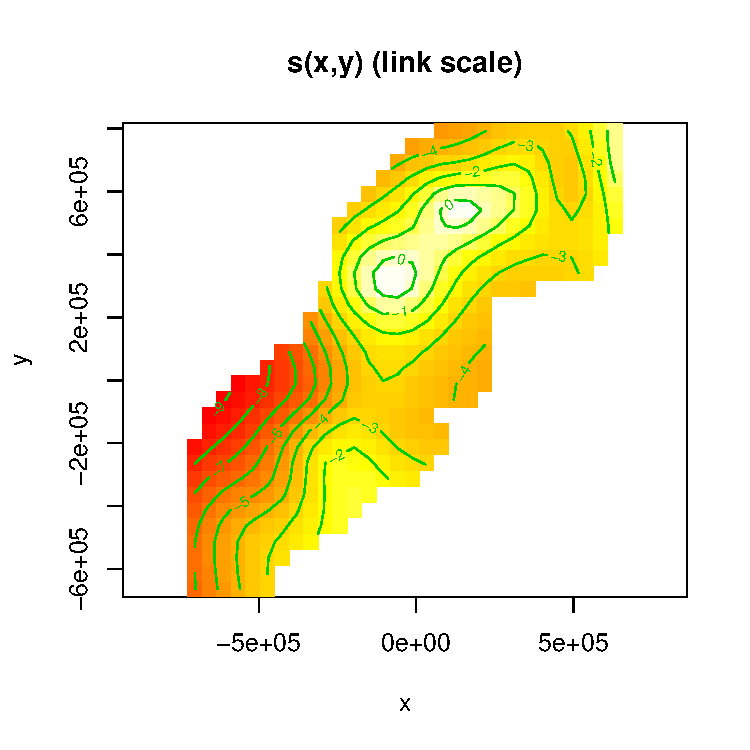
\includegraphics{_main_files/figure-latex/nb-xy-visgam-1.pdf}
\caption{\label{fig:nb-xy-visgam}Fitted surface (on link scale) for s(x,y)}
\end{figure}

Notes:

\begin{enumerate}
\def\labelenumi{\arabic{enumi}.}
\tightlist
\item
  The plot is on the scale of the link function, the offset is not taken
  into account -- the contour values do not represent abundance, just
  the ``influence'' of the smooth.
\item
  We set \texttt{view=c("x","y")} to display the smooths for \texttt{x}
  and \texttt{y} (we can choose any two variables in our model to
  display like this)
\item
  \texttt{plot.type="contour"} gives this ``flat'' plot, set
  \texttt{plot.type="persp"} for a ``perspective'' plot, in 3D.
\item
  The \texttt{too.far=0.1} argument displays the values of the smooth
  not ``too far'' from the data (try changing this value to see what
  happens).
\item
  \texttt{asp=1} ensures that the aspect ratio of the plot is 1, making
  the pixels square.
\item
  Read the \texttt{?vis.gam} manual page for more information on the
  plotting options.
\end{enumerate}

\subsection{Checking the model}\label{checking-the-model}

We can use the \texttt{gam.check()} and \texttt{rqgam.check} functions
to check the model.

\begin{Shaded}
\begin{Highlighting}[]
\KeywordTok{gam.check}\NormalTok{(dsm_nb_xy)}
\end{Highlighting}
\end{Shaded}

\begin{figure}
\centering
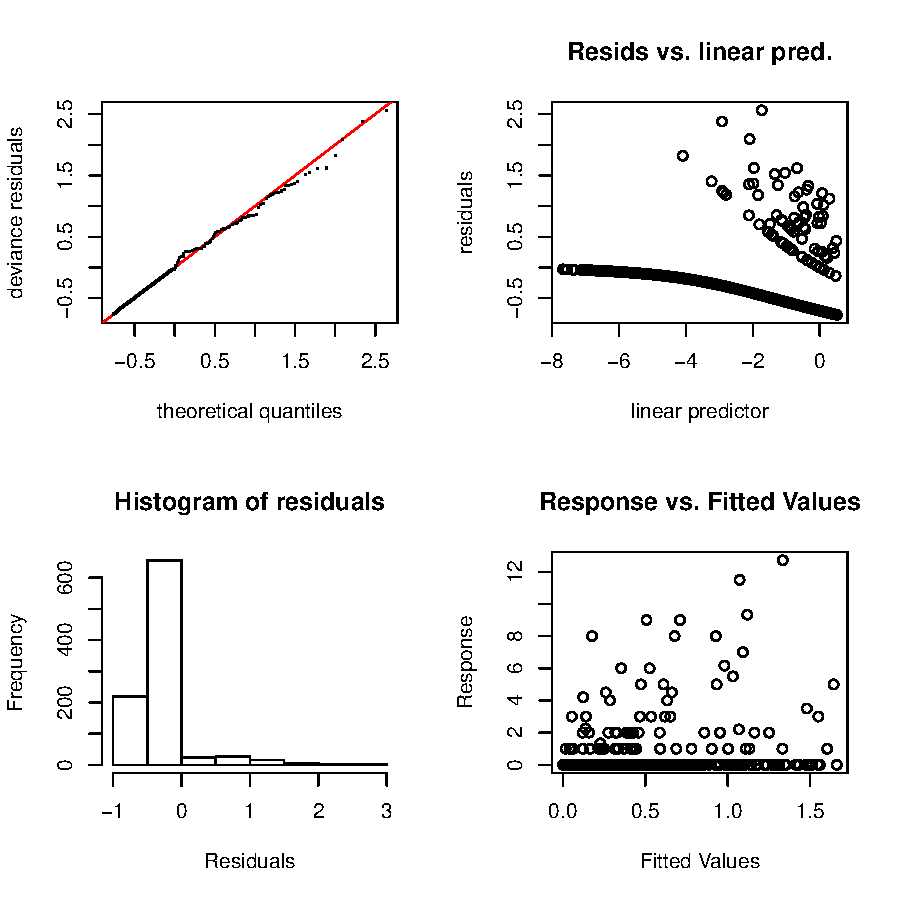
\includegraphics{_main_files/figure-latex/nb-xy-check-1.pdf}
\caption{\label{fig:nb-xy-check}Gam check results s(x,y) neg-binomial.}
\end{figure}

\begin{verbatim}
## 
## Method: REML   Optimizer: outer newton
## full convergence after 5 iterations.
## Gradient range [-4.081497e-08,5.889688e-08]
## (score 392.646 & scale 1).
## Hessian positive definite, eigenvalue range [2.157927,29.21001].
## Model rank =  30 / 30 
## 
## Basis dimension (k) checking results. Low p-value (k-index<1) may
## indicate that k is too low, especially if edf is close to k'.
## 
##        k' edf k-index p-value    
## s(x,y) 29  18    0.53  <2e-16 ***
## ---
## Signif. codes:  0 '***' 0.001 '**' 0.01 '*' 0.05 '.' 0.1 ' ' 1
\end{verbatim}

\begin{Shaded}
\begin{Highlighting}[]
\KeywordTok{rqgam.check}\NormalTok{(dsm_nb_xy, }\DataTypeTok{pch=}\DecValTok{20}\NormalTok{)}
\end{Highlighting}
\end{Shaded}

\begin{figure}
\centering
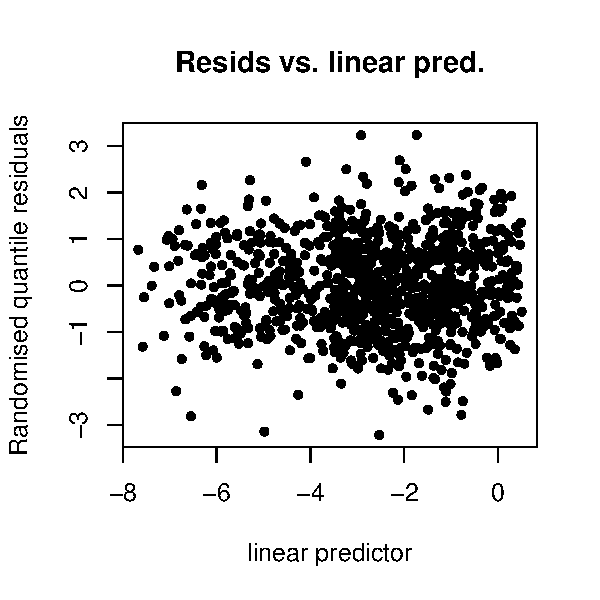
\includegraphics{_main_files/figure-latex/nb-xy-rqcheck-1.pdf}
\caption{\label{fig:nb-xy-rqcheck}Residual quartile gam check results s(x,y)
neg-binomial.}
\end{figure}

Remember that the left side of the \texttt{gam.check()} plot and the
right side of the \texttt{rqgam.check()} plot are most useful.

Looking back through the lecture notes, do you see any problems in these
plots or in the text output from \texttt{gam.check()}.

\subsection{Setting basis complexity}\label{setting-basis-complexity}

We can set the basis complexity via the \texttt{k} argument to the
\texttt{s()} term in the formula. For example the following re-fits the
above model with a much smaller basis complexity than before:

\begin{Shaded}
\begin{Highlighting}[]
\NormalTok{dsm_nb_xy_smallk <-}\StringTok{ }\KeywordTok{dsm}\NormalTok{(count}\OperatorTok{~}\KeywordTok{s}\NormalTok{(x, y, }\DataTypeTok{k=}\DecValTok{10}\NormalTok{),}
                        \DataTypeTok{ddf.obj=}\NormalTok{df_hn, }\DataTypeTok{segment.data =}\NormalTok{ segs, }\DataTypeTok{observation.data=}\NormalTok{obs,}
                        \DataTypeTok{family=}\KeywordTok{nb}\NormalTok{(), }\DataTypeTok{method=}\StringTok{"REML"}\NormalTok{)}
\end{Highlighting}
\end{Shaded}

Compare the output of \texttt{vis.gam()} and \texttt{gam.check()} for
this model to the model with a larger basis complexity.

\section{Estimated abundance as
response}\label{estimated-abundance-as-response}

So far we've just used \texttt{count} as the response. That is, we
adjusted the offset of the model to make it take into account the
``effective area'' of the segments (see lecture notes for a refresher).

Instead of using \texttt{count} we could use \texttt{abundance.est},
which will leave the segment areas as they are and calculate the
Horvitz-Thompson estimates of the abundance per segment and use that as
the response in the model. This is most useful when we have covariates
in the detection function (though we can use it any time).

Try copying the code that fits the model \texttt{dsm\_nb\_xy} and make a
model \texttt{dsm\_nb\_xy\_ae} that replaces \texttt{count} for
\texttt{abundance.est} in the model formula and uses the
\texttt{df\_hr\_ss\_size} detection function. Compare the results of
summaries, plots and checks between this and the count model.

\section{Univariate models}\label{univariate-models}

Instead of fitting a bivariate smooth of \texttt{x} and \texttt{y} using
\texttt{s(x,\ y)}, we could instead use the additive nature and fit the
following model:

\begin{Shaded}
\begin{Highlighting}[]
\NormalTok{dsm_nb_x_y <-}\StringTok{ }\KeywordTok{dsm}\NormalTok{(count}\OperatorTok{~}\KeywordTok{s}\NormalTok{(x)}\OperatorTok{+}\StringTok{ }\KeywordTok{s}\NormalTok{(y),}
                 \DataTypeTok{ddf.obj=}\NormalTok{df_hn, }\DataTypeTok{segment.data =}\NormalTok{ segs, }\DataTypeTok{observation.data=}\NormalTok{obs,}
                 \DataTypeTok{family=}\KeywordTok{nb}\NormalTok{(), }\DataTypeTok{method=}\StringTok{"REML"}\NormalTok{)}
\end{Highlighting}
\end{Shaded}

Compare this model with \texttt{dsm\_nb\_xy} using \texttt{vis.gam()}
(Note you can display two plots side-by-side using
\texttt{par(mfrow=c(1,2))}). Investigate the output from
\texttt{summary()} and the check functions too, comparing with the other
models, adjust \texttt{k} if necessary.

\section{Tweedie response
distribution}\label{tweedie-response-distribution}

So far, we've used \texttt{nb()} as the response -- the negative
binomial distribution. We can also try out the Tweedie distribution as a
response by replacing \texttt{nb()} with \texttt{tw()}.

Try this out and compare the resulting check plots.

\section{Save models}\label{save-models}

It'll be interesting to see how these models compare to the more complex
models we'll see later on. Let's save the fitted models at this stage.

\begin{Shaded}
\begin{Highlighting}[]
\CommentTok{# add your models here}
\KeywordTok{save}\NormalTok{(dsm_nb_x_y, dsm_nb_xy,}
     \DataTypeTok{file=}\StringTok{"dsms-xy.RData"}\NormalTok{)}
\end{Highlighting}
\end{Shaded}

\section{Extra credit}\label{extra-credit}

If you have time, try the following:

\begin{itemize}
\tightlist
\item
  What happens when we set \texttt{family=quasipoisson()}? Compare
  results of \texttt{gam.check} and \texttt{rqgam.check} for this and
  the other models.
\item
  Make the \texttt{k} value very big (\textasciitilde{}100 or so), what
  do you notice?
\end{itemize}

\chapter{Advanced density surface
models}\label{advanced-density-surface-models}

\section{Aims}\label{aims-3}

By the end of this practical, you should feel comfortable:

\begin{itemize}
\tightlist
\item
  Fitting DSMs with multiple smooth terms in them
\item
  Selecting smooth terms by \(p\)-values
\item
  Using shrinkage smoothers
\item
  Selecting between models using deviance, REML score
\item
  Investigating concurvity in DSMs with multiple smooths
\item
  Investigating sensitivity sensitivity and path dependence
\end{itemize}

\section{Load data and packages}\label{load-data-and-packages}

\begin{Shaded}
\begin{Highlighting}[]
\KeywordTok{library}\NormalTok{(Distance)}
\KeywordTok{library}\NormalTok{(dsm)}
\KeywordTok{library}\NormalTok{(ggplot2)}
\KeywordTok{library}\NormalTok{(knitr)}
\KeywordTok{library}\NormalTok{(kableExtra)}
\KeywordTok{library}\NormalTok{(plyr)}
\end{Highlighting}
\end{Shaded}

\begin{verbatim}
## 
## Attaching package: 'plyr'
\end{verbatim}

\begin{verbatim}
## The following object is masked from 'package:secr':
## 
##     join
\end{verbatim}

\begin{Shaded}
\begin{Highlighting}[]
\KeywordTok{library}\NormalTok{(reshape2)}
\end{Highlighting}
\end{Shaded}

Loading the data processed from GIS and the fitted detection function
objects from the previous exercises:

\begin{Shaded}
\begin{Highlighting}[]
\KeywordTok{load}\NormalTok{(}\StringTok{"sperm-data.RData"}\NormalTok{)}
\KeywordTok{load}\NormalTok{(}\StringTok{"df-models.RData"}\NormalTok{)}
\end{Highlighting}
\end{Shaded}

\section{Exploratory analysis}\label{exploratory-analysis-1}

We can do some exploratory analysis by aggregating the counts to each
cell and plotting what's going on.

\emph{Don't worry about understanding what this code is doing at the
moment.}

\begin{Shaded}
\begin{Highlighting}[]
\CommentTok{# join the observations onto the segments}
\NormalTok{join_dat <-}\StringTok{ }\KeywordTok{join}\NormalTok{(segs, obs, }\DataTypeTok{by=}\StringTok{"Sample.Label"}\NormalTok{, }\DataTypeTok{type=}\StringTok{"full"}\NormalTok{)}
\CommentTok{# sum up the observations per segment}
\NormalTok{n <-}\StringTok{ }\KeywordTok{ddply}\NormalTok{(join_dat, .(Sample.Label), summarise, }\DataTypeTok{n=}\KeywordTok{sum}\NormalTok{(size), }\DataTypeTok{.drop =} \OtherTok{FALSE}\NormalTok{) }
\CommentTok{# sort the segments by their labsl}
\NormalTok{segs_eda <-}\StringTok{ }\NormalTok{segs[}\KeywordTok{sort}\NormalTok{(segs}\OperatorTok{$}\NormalTok{Sample.Label),]}
\CommentTok{# make a new column for the counts}
\NormalTok{segs_eda}\OperatorTok{$}\NormalTok{n <-}\StringTok{ }\NormalTok{n}\OperatorTok{$}\NormalTok{n}

\CommentTok{# remove the columns we don't need,}
\NormalTok{segs_eda}\OperatorTok{$}\NormalTok{CentreTime <-}\StringTok{ }\OtherTok{NULL}
\NormalTok{segs_eda}\OperatorTok{$}\NormalTok{POINT_X <-}\StringTok{ }\OtherTok{NULL}
\NormalTok{segs_eda}\OperatorTok{$}\NormalTok{POINT_Y <-}\StringTok{ }\OtherTok{NULL}
\NormalTok{segs_eda}\OperatorTok{$}\NormalTok{segment.area <-}\StringTok{ }\OtherTok{NULL}
\NormalTok{segs_eda}\OperatorTok{$}\NormalTok{off.set <-}\StringTok{ }\OtherTok{NULL}
\NormalTok{segs_eda}\OperatorTok{$}\NormalTok{CenterTime <-}\StringTok{ }\OtherTok{NULL}
\NormalTok{segs_eda}\OperatorTok{$}\NormalTok{Effort <-}\StringTok{ }\OtherTok{NULL}
\NormalTok{segs_eda}\OperatorTok{$}\NormalTok{Length <-}\StringTok{ }\OtherTok{NULL}
\NormalTok{segs_eda}\OperatorTok{$}\NormalTok{SegmentID <-}\StringTok{ }\OtherTok{NULL}
\NormalTok{segs_eda}\OperatorTok{$}\NormalTok{coords.x1 <-}\StringTok{ }\OtherTok{NULL}
\NormalTok{segs_eda}\OperatorTok{$}\NormalTok{coords.x2 <-}\StringTok{ }\OtherTok{NULL}

\CommentTok{# "melt" the data so we have four columns:}
\CommentTok{#   Sample.Label, n (number of observations),}
\CommentTok{#   variable (which variable), value (its value)}
\NormalTok{segs_eda <-}\StringTok{ }\KeywordTok{melt}\NormalTok{(segs_eda, }\DataTypeTok{id.vars=}\KeywordTok{c}\NormalTok{(}\StringTok{"Sample.Label"}\NormalTok{, }\StringTok{"n"}\NormalTok{))}
\CommentTok{# try head(segs_eda)}
\end{Highlighting}
\end{Shaded}

Finally, we can plot histograms of counts for different values of the
covariates:

\begin{Shaded}
\begin{Highlighting}[]
\NormalTok{p <-}\StringTok{ }\KeywordTok{ggplot}\NormalTok{(segs_eda) }\OperatorTok{+}
\StringTok{       }\KeywordTok{geom_histogram}\NormalTok{(}\KeywordTok{aes}\NormalTok{(value, }\DataTypeTok{weight=}\NormalTok{n)) }\OperatorTok{+}
\StringTok{       }\KeywordTok{facet_wrap}\NormalTok{(}\OperatorTok{~}\NormalTok{variable, }\DataTypeTok{scale=}\StringTok{"free"}\NormalTok{) }\OperatorTok{+}
\StringTok{       }\KeywordTok{xlab}\NormalTok{(}\StringTok{"Covariate value"}\NormalTok{) }\OperatorTok{+}
\StringTok{       }\KeywordTok{ylab}\NormalTok{(}\StringTok{"Aggregated counts"}\NormalTok{)}
\end{Highlighting}
\end{Shaded}

\begin{verbatim}
## Warning: Ignoring unknown aesthetics: weight
\end{verbatim}

\begin{Shaded}
\begin{Highlighting}[]
\KeywordTok{print}\NormalTok{(p)}
\end{Highlighting}
\end{Shaded}

\begin{verbatim}
## `stat_bin()` using `bins = 30`. Pick better value with `binwidth`.
\end{verbatim}

\begin{figure}
\centering
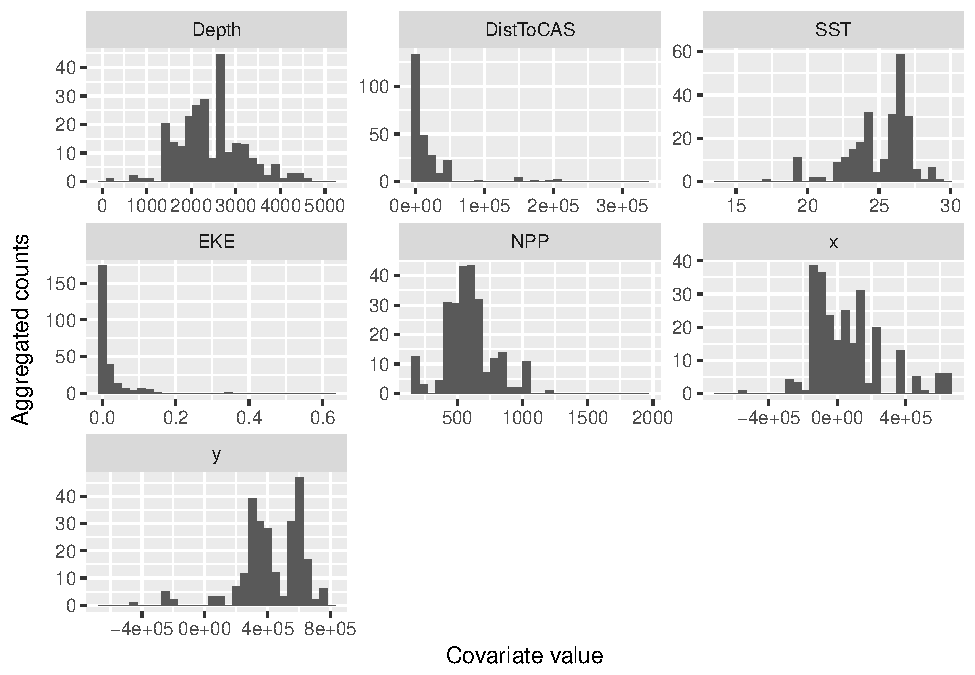
\includegraphics{_main_files/figure-latex/histcovar-1.pdf}
\caption{\label{fig:histcovar}Histograms of segment counts at various
covariate levels.}
\end{figure}

We can also just plot the counts against the covariates, note the high
number of zeros (but still some interesting patterns):

\begin{Shaded}
\begin{Highlighting}[]
\NormalTok{p <-}\StringTok{ }\KeywordTok{ggplot}\NormalTok{(segs_eda) }\OperatorTok{+}
\StringTok{       }\KeywordTok{geom_point}\NormalTok{(}\KeywordTok{aes}\NormalTok{(value, n)) }\OperatorTok{+}
\StringTok{       }\KeywordTok{facet_wrap}\NormalTok{(}\OperatorTok{~}\NormalTok{variable, }\DataTypeTok{scale=}\StringTok{"free"}\NormalTok{) }\OperatorTok{+}
\StringTok{       }\KeywordTok{xlab}\NormalTok{(}\StringTok{"Covariate value"}\NormalTok{) }\OperatorTok{+}
\StringTok{       }\KeywordTok{ylab}\NormalTok{(}\StringTok{"Aggregated counts"}\NormalTok{)}
\KeywordTok{print}\NormalTok{(p)}
\end{Highlighting}
\end{Shaded}

\begin{verbatim}
## Warning: Removed 6076 rows containing missing values (geom_point).
\end{verbatim}

\begin{figure}
\centering
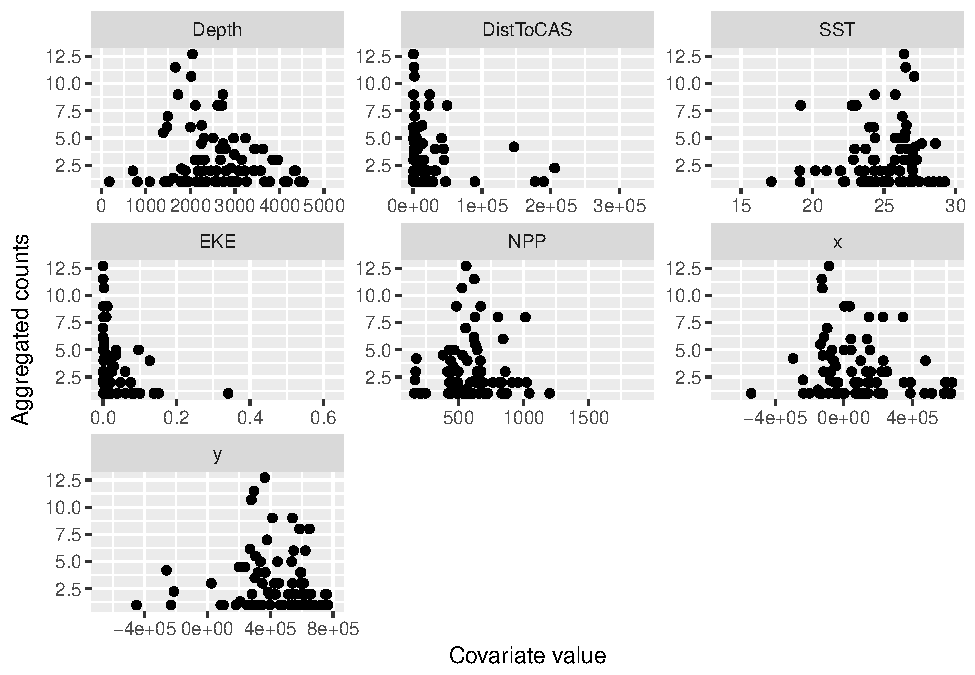
\includegraphics{_main_files/figure-latex/countcovar-1.pdf}
\caption{\label{fig:countcovar}Relationship of segment counts to covariate
values.}
\end{figure}

These plots give a very rough idea of the relationships we can expect in
the model. Notably these plots don't take into account interactions
between the variables and potential correlations between the terms, as
well as detectability.

\section{Pre-model fitting}\label{pre-model-fitting-1}

As we did in the previous exercise we must remove the observations from
the spatial data that we excluded when we fitted the detection function
-- those observations at distances greater than the truncation.

\begin{Shaded}
\begin{Highlighting}[]
\NormalTok{obs <-}\StringTok{ }\NormalTok{obs[obs}\OperatorTok{$}\NormalTok{distance }\OperatorTok{<=}\StringTok{ }\NormalTok{df_hn}\OperatorTok{$}\NormalTok{ddf}\OperatorTok{$}\NormalTok{meta.data}\OperatorTok{$}\NormalTok{width,]}
\end{Highlighting}
\end{Shaded}

Here we've used the value of the truncation stored in the detection
function object, but we could also use the numeric value (which we can
also find by checking the model's \texttt{summary()}).

Again note that if you want to fit DSMs using detection functions with
different truncation distances, then you'll need to reload the
\texttt{sperm-data.RData} and do the truncation again for that detection
function.

\section{\texorpdfstring{Our new friend
\texttt{+}}{Our new friend +}}\label{our-new-friend}

We can build a really big model using \texttt{+} to include all the
terms that we want in the model. We can check what's available to us by
using \texttt{head()} to look at the segment table:

\begin{Shaded}
\begin{Highlighting}[]
\KeywordTok{head}\NormalTok{(segs)}
\end{Highlighting}
\end{Shaded}

\begin{verbatim}
##            CenterTime SegmentID   Length  POINT_X  POINT_Y     Depth
## 1 2004/06/24 07:27:04         1 10288.91 214544.0 689074.3  118.5027
## 2 2004/06/24 08:08:04         2 10288.91 222654.3 682781.0  119.4853
## 3 2004/06/24 09:03:18         3 10288.91 230279.9 675473.3  177.2779
## 4 2004/06/24 09:51:27         4 10288.91 239328.9 666646.3  527.9562
## 5 2004/06/24 10:25:39         5 10288.91 246686.5 659459.2  602.6378
## 6 2004/06/24 11:00:22         6 10288.91 254307.0 652547.2 1094.4402
##    DistToCAS      SST          EKE      NPP coords.x1 coords.x2        x
## 1 14468.1533 15.54390 0.0014442616 1908.129  214544.0  689074.3 214544.0
## 2 10262.9648 15.88358 0.0014198086 1889.540  222654.3  682781.0 222654.3
## 3  6900.9829 16.21920 0.0011704842 1842.057  230279.9  675473.3 230279.9
## 4  1055.4124 16.45468 0.0004101589 1823.942  239328.9  666646.3 239328.9
## 5  1112.6293 16.62554 0.0002553244 1721.949  246686.5  659459.2 246686.5
## 6   707.5795 16.83725 0.0006556266 1400.281  254307.0  652547.2 254307.0
##          y   Effort Sample.Label
## 1 689074.3 10288.91            1
## 2 682781.0 10288.91            2
## 3 675473.3 10288.91            3
## 4 666646.3 10288.91            4
## 5 659459.2 10288.91            5
## 6 652547.2 10288.91            6
\end{verbatim}

We can then fit a model with the available covariates in it, each as an
\texttt{s()} term.

\begin{Shaded}
\begin{Highlighting}[]
\NormalTok{dsm_nb_xy_ms <-}\StringTok{ }\KeywordTok{dsm}\NormalTok{(count}\OperatorTok{~}\KeywordTok{s}\NormalTok{(x,y, }\DataTypeTok{bs=}\StringTok{"ts"}\NormalTok{) }\OperatorTok{+}
\StringTok{                       }\KeywordTok{s}\NormalTok{(Depth, }\DataTypeTok{bs=}\StringTok{"ts"}\NormalTok{) }\OperatorTok{+}
\StringTok{                       }\KeywordTok{s}\NormalTok{(DistToCAS, }\DataTypeTok{bs=}\StringTok{"ts"}\NormalTok{) }\OperatorTok{+}
\StringTok{                       }\KeywordTok{s}\NormalTok{(SST, }\DataTypeTok{bs=}\StringTok{"ts"}\NormalTok{) }\OperatorTok{+}
\StringTok{                       }\KeywordTok{s}\NormalTok{(EKE, }\DataTypeTok{bs=}\StringTok{"ts"}\NormalTok{) }\OperatorTok{+}
\StringTok{                       }\KeywordTok{s}\NormalTok{(NPP, }\DataTypeTok{bs=}\StringTok{"ts"}\NormalTok{),}
\NormalTok{                 df_hn, segs, obs,}
                 \DataTypeTok{family=}\KeywordTok{nb}\NormalTok{(), }\DataTypeTok{method=}\StringTok{"REML"}\NormalTok{)}
\KeywordTok{summary}\NormalTok{(dsm_nb_xy_ms)}
\end{Highlighting}
\end{Shaded}

\begin{verbatim}
## 
## Family: Negative Binomial(0.114) 
## Link function: log 
## 
## Formula:
## count ~ s(x, y, bs = "ts") + s(Depth, bs = "ts") + s(DistToCAS, 
##     bs = "ts") + s(SST, bs = "ts") + s(EKE, bs = "ts") + s(NPP, 
##     bs = "ts") + offset(off.set)
## 
## Parametric coefficients:
##             Estimate Std. Error z value Pr(>|z|)    
## (Intercept) -20.7732     0.2295   -90.5   <2e-16 ***
## ---
## Signif. codes:  0 '***' 0.001 '**' 0.01 '*' 0.05 '.' 0.1 ' ' 1
## 
## Approximate significance of smooth terms:
##                    edf Ref.df Chi.sq  p-value    
## s(x,y)       1.8636924     29 19.141 2.90e-05 ***
## s(Depth)     3.4176460      9 46.263 1.65e-11 ***
## s(DistToCAS) 0.0000801      9  0.000   0.9053    
## s(SST)       0.0002076      9  0.000   0.5402    
## s(EKE)       0.8563344      9  5.172   0.0134 *  
## s(NPP)       0.0001018      9  0.000   0.7820    
## ---
## Signif. codes:  0 '***' 0.001 '**' 0.01 '*' 0.05 '.' 0.1 ' ' 1
## 
## R-sq.(adj) =  0.0947   Deviance explained = 39.2%
## -REML = 382.76  Scale est. = 1         n = 949
\end{verbatim}

Notes:

\begin{enumerate}
\def\labelenumi{\arabic{enumi}.}
\tightlist
\item
  We're using \texttt{bs="ts"} to use the shrinkage thin plate
  regression spline. More technical detail on these smooths can be found
  on their manual page \texttt{?smooth.construct.ts.smooth.spec}.
\item
  We've not specified basis complexity (\texttt{k}) at the moment. Note
  that if you want to specify the same complexity for multiple terms,
  it's often easier to make a variable that can then be given as
  \texttt{k} (for example, setting \texttt{k1\textless{}-15} and then
  setting \texttt{k=k1} in the required \texttt{s()} terms).
\end{enumerate}

\subsection{Plot}\label{plot}

Let's plot the smooths from this model:

\begin{Shaded}
\begin{Highlighting}[]
\KeywordTok{plot}\NormalTok{(dsm_nb_xy_ms, }\DataTypeTok{pages=}\DecValTok{1}\NormalTok{, }\DataTypeTok{scale=}\DecValTok{0}\NormalTok{)}
\end{Highlighting}
\end{Shaded}

\begin{figure}
\centering
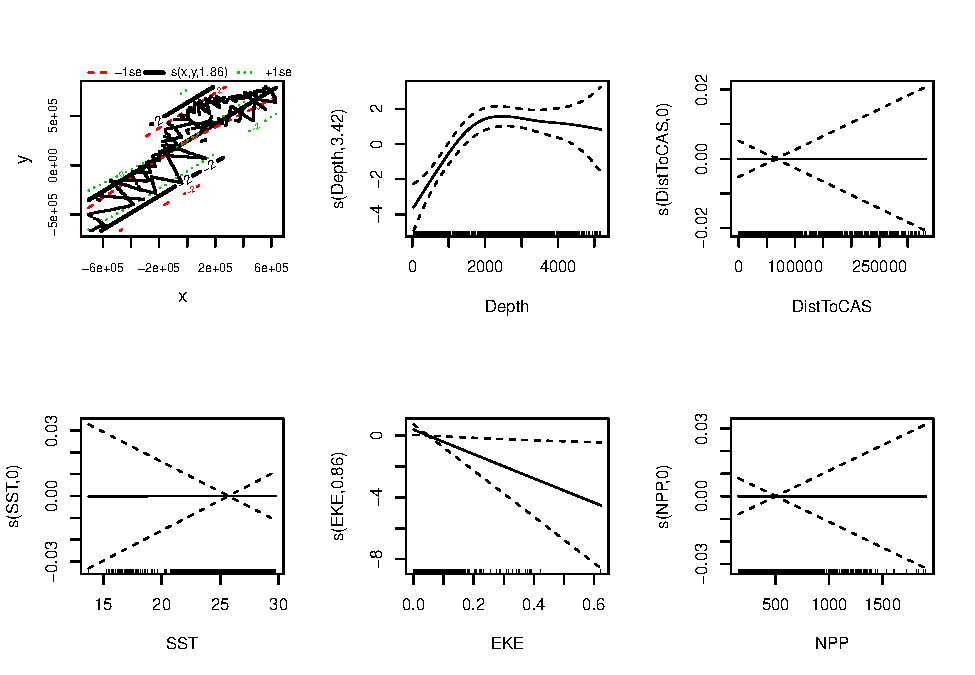
\includegraphics{_main_files/figure-latex/plot-nb-xy-1.pdf}
\caption{\label{fig:plot-nb-xy}Smooths for all covariates with neg-binomial
response distribution.}
\end{figure}

Notes:

\begin{enumerate}
\def\labelenumi{\arabic{enumi}.}
\tightlist
\item
  Setting \texttt{shade=TRUE} gives prettier confidence bands.
\item
  As with \texttt{vis.gam()} the response is on the link scale.
\item
  \texttt{scale=0} puts each plot on a different \(y\)-axis scale,
  making it easier to see the effects. Setting \texttt{scale=-1} will
  put the plots on a common \(y\)-axis scale
\end{enumerate}

We can also plot the bivariate smooth of \texttt{x} and \texttt{y} as we
did before, using \texttt{vis.gam()}:

\begin{Shaded}
\begin{Highlighting}[]
\KeywordTok{vis.gam}\NormalTok{(dsm_nb_xy_ms, }\DataTypeTok{view=}\KeywordTok{c}\NormalTok{(}\StringTok{"x"}\NormalTok{,}\StringTok{"y"}\NormalTok{), }\DataTypeTok{plot.type=}\StringTok{"contour"}\NormalTok{, }\DataTypeTok{too.far=}\FloatTok{0.1}\NormalTok{, }
        \DataTypeTok{main=}\StringTok{"s(x,y) (link scale)"}\NormalTok{, }\DataTypeTok{asp=}\DecValTok{1}\NormalTok{)}
\end{Highlighting}
\end{Shaded}

\begin{figure}
\centering
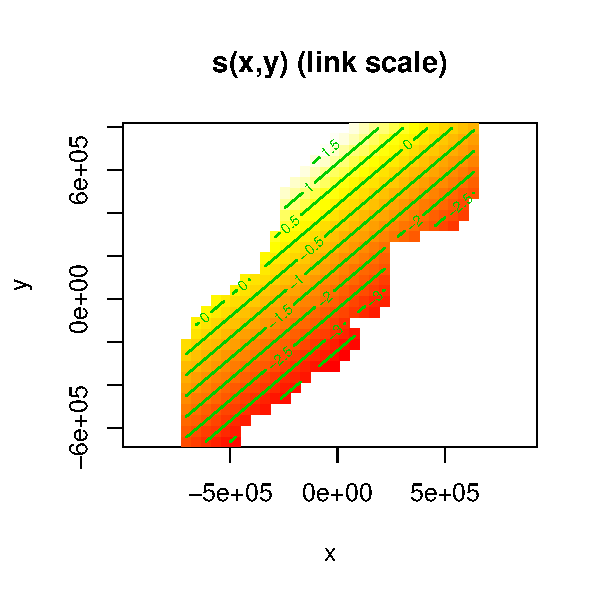
\includegraphics{_main_files/figure-latex/nb-xy-visgam-03-1.pdf}
\caption{\label{fig:nb-xy-visgam-03}Fitted surface with all environmental
covariates, and neg-binomial response distribution.}
\end{figure}

Compare this plot to Figure \ref{fig:nb-xy-visgam}, generated in the
previous practical when only \texttt{x} and \texttt{y} were included in
the model.

\subsection{Check}\label{check}

As before, we can use \texttt{gam.check()} and \texttt{rqgam.check()} to
look at the residual check plots for this model. Do this in the below
gaps and comment on the resulting plots and diagnostics.

You might decide from the diagnostics that you need to increase
\texttt{k} for some of the terms in the model. Do this and re-run the
above code to ensure that the smooths are flexible enough. The
\texttt{?choose.k} manual page can offer some guidance. Generally if the
EDF is close to the value of \texttt{k} you supplied, it's worth
doubling \texttt{k} and refitting to see what happens. You can always
switch back to the smaller \texttt{k} if there is little difference.

\subsection{Select terms}\label{select-terms}

As was covered in the lectures, we can select terms by (approximate)
\(p\)-values and by looking for terms that have EDFs significantly less
than 1 (those which have been shrunk).

Decide on a significance level that you'll use to discard terms in the
model. Remove the terms that are non-significant at this level and
re-run the above checks, summaries and plots to see what happens. It's
helpful to make notes to yourself as you go

It's easiest to either comment out the terms that are to be removed
(using \texttt{\#}) or by copying the code chunk above and pasting it
below.

Having removed a smooth and reviewed your model, you may decide you wish
to remove another. Follow the process again, removing a term, looking at
plots and diagnostics.

\subsection{Compare response
distributions}\label{compare-response-distributions}

Use the \texttt{gam.check()} to compare quantile-quantile plots between
negative binomial and Tweedie distributions for the response.

\section{Estimated abundance as a
response}\label{estimated-abundance-as-a-response}

Again, we've only looked at models with \texttt{count} as the response.
Try using a detection function with covariates and the
\texttt{abundance.est} response in the chunk below:

\section{Concurvity}\label{concurvity}

Checking concurvity (Amodio, Aria, and D'Ambrosio
(\protect\hyperlink{ref-Amodio2014}{2014})) of terms in the model can be
accomplished using the \texttt{concurvity()} function.

\begin{Shaded}
\begin{Highlighting}[]
\KeywordTok{concurvity}\NormalTok{(dsm_nb_xy_ms)}
\end{Highlighting}
\end{Shaded}

\begin{verbatim}
##                  para    s(x,y)  s(Depth) s(DistToCAS)    s(SST)    s(EKE)
## worst    9.804613e-24 0.9963493 0.9836597    0.9959057 0.9772853 0.7702479
## observed 9.804613e-24 0.8597372 0.8277050    0.9879372 0.9523512 0.6746585
## estimate 9.804613e-24 0.7580838 0.9272203    0.9642030 0.8978412 0.4906765
##             s(NPP)
## worst    0.9727752
## observed 0.9525363
## estimate 0.8694619
\end{verbatim}

By default the function returns a matrix of a measure of concurvity
between one of the terms and the rest of the model.

Compare the output of the models before and after removing terms.

Reading these matrices can be laborious and not very fun. The function
\texttt{vis.concurvity()} in the \texttt{dsm} package is used to
visualise the concurvity \emph{between terms} in a model by colour
coding the matrix (and blanking out the redundant information).

Again compare the results of plotting for models with different terms.

\section{Sensitivity}\label{sensitivity}

\subsection{Compare bivariate and additive spatial
effects}\label{compare-bivariate-and-additive-spatial-effects}

If we replace the bivariate smooth of location (\texttt{s(x,\ y)}) with
an additive terms (\texttt{s(x)+s(y)}), we may see a difference in the
final model (different covariates selected).

\begin{Shaded}
\begin{Highlighting}[]
\NormalTok{dsm_nb_x_y_ms <-}\StringTok{ }\KeywordTok{dsm}\NormalTok{(count}\OperatorTok{~}\KeywordTok{s}\NormalTok{(x, }\DataTypeTok{bs=}\StringTok{"ts"}\NormalTok{) }\OperatorTok{+}
\StringTok{                        }\KeywordTok{s}\NormalTok{(y, }\DataTypeTok{bs=}\StringTok{"ts"}\NormalTok{) }\OperatorTok{+}
\StringTok{                        }\KeywordTok{s}\NormalTok{(Depth, }\DataTypeTok{bs=}\StringTok{"ts"}\NormalTok{) }\OperatorTok{+}
\StringTok{                        }\KeywordTok{s}\NormalTok{(DistToCAS, }\DataTypeTok{bs=}\StringTok{"ts"}\NormalTok{) }\OperatorTok{+}
\StringTok{                        }\KeywordTok{s}\NormalTok{(SST, }\DataTypeTok{bs=}\StringTok{"ts"}\NormalTok{) }\OperatorTok{+}
\StringTok{                        }\KeywordTok{s}\NormalTok{(EKE, }\DataTypeTok{bs=}\StringTok{"ts"}\NormalTok{) }\OperatorTok{+}
\StringTok{                        }\KeywordTok{s}\NormalTok{(NPP, }\DataTypeTok{bs=}\StringTok{"ts"}\NormalTok{),}
\NormalTok{                  df_hn, segs, obs,}
                  \DataTypeTok{family=}\KeywordTok{nb}\NormalTok{(), }\DataTypeTok{method=}\StringTok{"REML"}\NormalTok{)}
\KeywordTok{summary}\NormalTok{(dsm_nb_x_y_ms)}
\end{Highlighting}
\end{Shaded}

\begin{verbatim}
## 
## Family: Negative Binomial(0.116) 
## Link function: log 
## 
## Formula:
## count ~ s(x, bs = "ts") + s(y, bs = "ts") + s(Depth, bs = "ts") + 
##     s(DistToCAS, bs = "ts") + s(SST, bs = "ts") + s(EKE, bs = "ts") + 
##     s(NPP, bs = "ts") + offset(off.set)
## 
## Parametric coefficients:
##             Estimate Std. Error z value Pr(>|z|)    
## (Intercept) -20.7743     0.2274  -91.37   <2e-16 ***
## ---
## Signif. codes:  0 '***' 0.001 '**' 0.01 '*' 0.05 '.' 0.1 ' ' 1
## 
## Approximate significance of smooth terms:
##                    edf Ref.df Chi.sq  p-value    
## s(x)         2.875e-01      9  0.337   0.2698    
## s(y)         1.709e-05      9  0.000   0.6304    
## s(Depth)     3.391e+00      9 37.216 9.88e-10 ***
## s(DistToCAS) 5.393e-04      9  0.000   0.5246    
## s(SST)       9.814e-05      9  0.000   0.8176    
## s(EKE)       8.670e-01      9  5.582   0.0103 *  
## s(NPP)       2.844e+00      9 23.236 9.13e-07 ***
## ---
## Signif. codes:  0 '***' 0.001 '**' 0.01 '*' 0.05 '.' 0.1 ' ' 1
## 
## R-sq.(adj) =  0.0993   Deviance explained = 40.7%
## -REML = 383.03  Scale est. = 1         n = 949
\end{verbatim}

Try performing model selection as before from this base model and
compare the resulting models.

Compare the resulting smooths from like terms in the model. For example,
if depth were selected in both models, compare EDFs and plots, e.g.:

\begin{Shaded}
\begin{Highlighting}[]
\KeywordTok{par}\NormalTok{(}\DataTypeTok{mfrow=}\KeywordTok{c}\NormalTok{(}\DecValTok{1}\NormalTok{,}\DecValTok{2}\NormalTok{))}
\KeywordTok{plot}\NormalTok{(dsm_nb_xy_ms, }\DataTypeTok{select=}\DecValTok{2}\NormalTok{)}
\KeywordTok{plot}\NormalTok{(dsm_nb_x_y_ms, }\DataTypeTok{select=}\DecValTok{3}\NormalTok{)}
\end{Highlighting}
\end{Shaded}

\begin{figure}
\centering
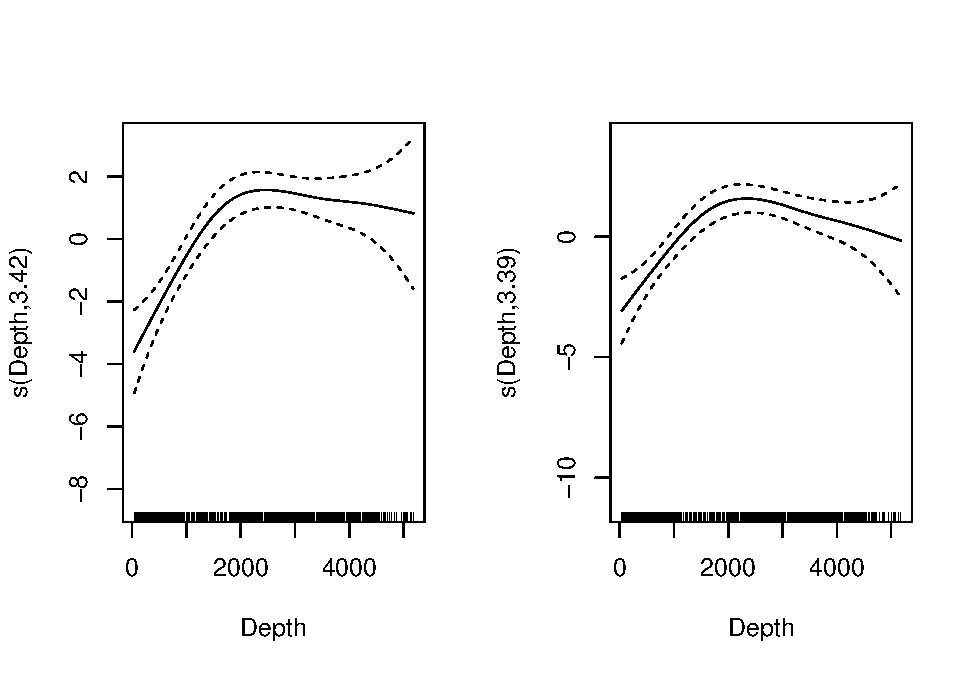
\includegraphics{_main_files/figure-latex/compare-depth-1.pdf}
\caption{\label{fig:compare-depth}Shape of depth covariate response with
bivariate s(x,y) and univariate s(x)+s(y).}
\end{figure}

Note that there \texttt{select=} picks just one term to plot. These are
in the order in which the terms occur in the \texttt{summary()} output
(so you may well need to adjust the above code).

\section{Comparing models}\label{comparing-models}

As with the detection functions in the earlier exercises, here is a
quick function to generate model results tables with appropriate summary
statistics:

\begin{Shaded}
\begin{Highlighting}[]
\NormalTok{summarize_dsm <-}\StringTok{ }\ControlFlowTok{function}\NormalTok{(model)\{}

\NormalTok{  summ <-}\StringTok{ }\KeywordTok{summary}\NormalTok{(model)}

  \KeywordTok{data.frame}\NormalTok{(}\DataTypeTok{response =}\NormalTok{ model}\OperatorTok{$}\NormalTok{family}\OperatorTok{$}\NormalTok{family,}
             \DataTypeTok{terms    =} \KeywordTok{paste}\NormalTok{(}\KeywordTok{rownames}\NormalTok{(summ}\OperatorTok{$}\NormalTok{s.table), }\DataTypeTok{collapse=}\StringTok{", "}\NormalTok{),}
             \DataTypeTok{AIC      =} \KeywordTok{AIC}\NormalTok{(model),}
             \DataTypeTok{REML     =}\NormalTok{ model}\OperatorTok{$}\NormalTok{gcv.ubre,}
             \StringTok{"Deviance_explained"}\NormalTok{ =}\StringTok{ }\KeywordTok{paste0}\NormalTok{(}\KeywordTok{round}\NormalTok{(summ}\OperatorTok{$}\NormalTok{dev.expl}\OperatorTok{*}\DecValTok{100}\NormalTok{,}\DecValTok{2}\NormalTok{),}\StringTok{"%"}\NormalTok{)}
\NormalTok{            )}

\NormalTok{\}}
\end{Highlighting}
\end{Shaded}

We can make a list of the models and pass the list to the above
function.

\begin{Shaded}
\begin{Highlighting}[]
\CommentTok{# add your models to this list!}
\NormalTok{model_list <-}\StringTok{ }\KeywordTok{list}\NormalTok{(dsm_nb_x_y_ms, dsm_nb_xy_ms)}
\KeywordTok{library}\NormalTok{(plyr)}
\NormalTok{summary_table <-}\StringTok{ }\KeywordTok{ldply}\NormalTok{(model_list, summarize_dsm)}
\KeywordTok{row.names}\NormalTok{(summary_table) <-}\StringTok{ }\KeywordTok{c}\NormalTok{(}\StringTok{"dsm_nb_x_y_ms"}\NormalTok{, }\StringTok{"dsm_nb_xy_ms"}\NormalTok{)}
\end{Highlighting}
\end{Shaded}

\begin{Shaded}
\begin{Highlighting}[]
\NormalTok{summary_table <-}\StringTok{ }\NormalTok{summary_table[}\KeywordTok{order}\NormalTok{(summary_table}\OperatorTok{$}\NormalTok{REML, }\DataTypeTok{decreasing=}\OtherTok{TRUE}\NormalTok{),]}
\KeywordTok{kable}\NormalTok{(summary_table, }
      \DataTypeTok{caption =} \StringTok{"Model performance of s(x,y) and s(x)+s(y) in presence of other covariates."}\NormalTok{) }\OperatorTok
\StringTok{  }\KeywordTok{kable_styling}\NormalTok{(}\DataTypeTok{latex_options=}\StringTok{"scale_down"}\NormalTok{)}
\end{Highlighting}
\end{Shaded}

\begin{table}

\caption{\label{tab:print-table-03}Model performance of s(x,y) and s(x)+s(y) in presence of other covariates.}
\centering
\resizebox{\linewidth}{!}{\begin{tabular}[t]{l|l|l|r|r|l}
\hline
  & response & terms & AIC & REML & Deviance\_explained\\
\hline
dsm\_nb\_x\_y\_ms & Negative Binomial(0.116) & s(x), s(y), s(Depth), s(DistToCAS), s(SST), s(EKE), s(NPP) & 752.5585 & 383.0326 & 40.73\%\\
\hline
dsm\_nb\_xy\_ms & Negative Binomial(0.114) & s(x,y), s(Depth), s(DistToCAS), s(SST), s(EKE), s(NPP) & 754.0326 & 382.7591 & 39.2\%\\
\hline
\end{tabular}}
\end{table}

\section{Saving models}\label{saving-models}

Now save the models that you'd like to use to predict with later. I
recommend saving as many models as you can so you can compare their
results in the next practical.

\begin{Shaded}
\begin{Highlighting}[]
\CommentTok{# add your models here}
\KeywordTok{save}\NormalTok{(dsm_nb_xy_ms, dsm_nb_x_y_ms,}
     \DataTypeTok{file=}\StringTok{"dsms.RData"}\NormalTok{)}
\end{Highlighting}
\end{Shaded}

\chapter{Prediction using fitted density surface
models}\label{prediction-using-fitted-density-surface-models}

Now we've fitted some models, let's use the \texttt{predict} functions
and the data from GIS to make predictions of abundance.

\section{Aims}\label{aims-4}

By the end of this practical, you should feel comfortable:

\begin{itemize}
\tightlist
\item
  Loading raster data into R
\item
  Building a \texttt{data.frame} of prediction covariates
\item
  Making a prediction using the \texttt{predict()} function
\item
  Summing the prediction cells to obtain a total abundance for a given
  area
\item
  Plotting a map of predictions
\item
  Saving predictions to a raster to be used in ArcGIS
\end{itemize}

\section{Loading the packages and
data}\label{loading-the-packages-and-data}

\begin{Shaded}
\begin{Highlighting}[]
\KeywordTok{library}\NormalTok{(knitr)}
\KeywordTok{library}\NormalTok{(dsm)}
\KeywordTok{library}\NormalTok{(ggplot2)}
\CommentTok{# colourblind-friendly colourschemes}
\KeywordTok{library}\NormalTok{(viridis)}
\end{Highlighting}
\end{Shaded}

\begin{verbatim}
## Loading required package: viridisLite
\end{verbatim}

\begin{Shaded}
\begin{Highlighting}[]
\CommentTok{# to load and save raster data}
\KeywordTok{library}\NormalTok{(raster)}
\end{Highlighting}
\end{Shaded}

\begin{verbatim}
## 
## Attaching package: 'raster'
\end{verbatim}

\begin{verbatim}
## The following object is masked from 'package:nlme':
## 
##     getData
\end{verbatim}

\begin{verbatim}
## The following objects are masked from 'package:secr':
## 
##     flip, rotate, shift, trim
\end{verbatim}

\begin{Shaded}
\begin{Highlighting}[]
\CommentTok{# models with only spatial terms}
\KeywordTok{load}\NormalTok{(}\StringTok{"dsms-xy.RData"}\NormalTok{)}
\CommentTok{# models with all covariates}
\KeywordTok{load}\NormalTok{(}\StringTok{"dsms.RData"}\NormalTok{)}
\end{Highlighting}
\end{Shaded}

\section{Loading prediction data}\label{loading-prediction-data}

Before we can make predictions we first need to load the covariates into
a ``stack'' from their files on disk using the \texttt{stack()} function
from \texttt{raster}. We give \texttt{stack()} a vector of locations to
load the rasters from. Note that in RStudio you can use tab-completion
for these locations and avoid some typing. At this point we arbitrarily
choose the time periods of the SST, NPP and EKE rasters (2 June 2004, or
Julian date 153).

\begin{Shaded}
\begin{Highlighting}[]
\NormalTok{predictorStack <-}\StringTok{ }\KeywordTok{stack}\NormalTok{(}\KeywordTok{c}\NormalTok{(}\StringTok{"../../spermwhale-analysis/Covariates_for_Study_Area/Depth.img"}\NormalTok{,}
                          \StringTok{"../../spermwhale-analysis/Covariates_for_Study_Area/GLOB/CMC/CMC0.2deg/analysed_sst/2004/20040602-CMC-L4SSTfnd-GLOB-v02-fv02.0-CMC0.2deg-analysed_sst.img"}\NormalTok{,}
                          \StringTok{"../../spermwhale-analysis/Covariates_for_Study_Area/VGPM/Rasters/vgpm.2004153.hdf.gz.img"}\NormalTok{,}
                          \StringTok{"../../spermwhale-analysis/Covariates_for_Study_Area/DistToCanyonsAndSeamounts.img"}\NormalTok{,}
                          \StringTok{"../../spermwhale-analysis/Covariates_for_Study_Area/Global/DT\textbackslash{} all\textbackslash{} sat/MSLA_ke/2004/MSLA_ke_2004153.img"}
\NormalTok{                          ))}
\end{Highlighting}
\end{Shaded}

We need to rename the layers in our stack to match those in the model we
are going to use to predict. If you need a refresher on the names that
were used there, call \texttt{summary()} on the DSM object.

\begin{Shaded}
\begin{Highlighting}[]
\KeywordTok{names}\NormalTok{(predictorStack) <-}\StringTok{ }\KeywordTok{c}\NormalTok{(}\StringTok{"Depth"}\NormalTok{,}\StringTok{"SST"}\NormalTok{,}\StringTok{"NPP"}\NormalTok{, }\StringTok{"DistToCAS"}\NormalTok{, }\StringTok{"EKE"}\NormalTok{)}
\end{Highlighting}
\end{Shaded}

Now these are loaded, we can coerce the stack into something
\texttt{dsm} can talk to using the \texttt{as.data.frame} function. Note
we need the \texttt{xy=TRUE} to ensure that \texttt{x} and \texttt{y}
are included in the prediction data. We also set the offset value -- the
area of each cell in our prediction grid.

\begin{Shaded}
\begin{Highlighting}[]
\NormalTok{predgrid <-}\StringTok{ }\KeywordTok{as.data.frame}\NormalTok{(predictorStack, }\DataTypeTok{xy=}\OtherTok{TRUE}\NormalTok{)}
\NormalTok{predgrid}\OperatorTok{$}\NormalTok{off.set <-}\StringTok{ }\NormalTok{(}\DecValTok{10}\OperatorTok{*}\DecValTok{1000}\NormalTok{)}\OperatorTok{^}\DecValTok{2}
\end{Highlighting}
\end{Shaded}

We can then predict for the model \texttt{dsm\_nb\_xy\_ms}:

\begin{Shaded}
\begin{Highlighting}[]
\NormalTok{pp <-}\StringTok{ }\KeywordTok{predict}\NormalTok{(dsm_nb_xy_ms, predgrid)}
\end{Highlighting}
\end{Shaded}

This is just a list of numbers -- the predicted abundance per cell. We
can sum these to get the estimated abundance for the study area:

\begin{Shaded}
\begin{Highlighting}[]
\KeywordTok{sum}\NormalTok{(pp, }\DataTypeTok{na.rm=}\OtherTok{TRUE}\NormalTok{)}
\end{Highlighting}
\end{Shaded}

\begin{verbatim}
## [1] 1710.347
\end{verbatim}

Because we predicted over the whole raster grid (including those cells
without covariate values -- e.g.~land), some of the values in
\texttt{pp} will be \texttt{NA}, so we can ignore them when we sum by
setting \texttt{na.rm=TRUE}. We need to do this again when we plot the
data too.

We can also plot this to get a spatial representation of the
predictions:

\begin{Shaded}
\begin{Highlighting}[]
\CommentTok{# assign the predictions to the prediction grid data.frame}
\NormalTok{predgrid}\OperatorTok{$}\NormalTok{Nhat_nb_xy <-}\StringTok{ }\NormalTok{pp}
\CommentTok{# remove the NA entries (because of the grid structure of the raster)}
\NormalTok{predgrid_plot <-}\StringTok{ }\NormalTok{predgrid[}\OperatorTok{!}\KeywordTok{is.na}\NormalTok{(predgrid}\OperatorTok{$}\NormalTok{Nhat_nb_xy),]}
\CommentTok{# plot!}
\NormalTok{p <-}\StringTok{ }\KeywordTok{ggplot}\NormalTok{(predgrid_plot) }\OperatorTok{+}
\StringTok{      }\KeywordTok{geom_tile}\NormalTok{(}\KeywordTok{aes}\NormalTok{(}\DataTypeTok{x=}\NormalTok{x, }\DataTypeTok{y=}\NormalTok{y, }\DataTypeTok{fill=}\NormalTok{Nhat_nb_xy, }\DataTypeTok{width=}\DecValTok{10}\OperatorTok{*}\DecValTok{1000}\NormalTok{, }\DataTypeTok{height=}\DecValTok{10}\OperatorTok{*}\DecValTok{1000}\NormalTok{)) }\OperatorTok{+}
\StringTok{      }\KeywordTok{coord_equal}\NormalTok{() }\OperatorTok{+}\StringTok{ }
\StringTok{      }\KeywordTok{scale_fill_viridis}\NormalTok{()}
\end{Highlighting}
\end{Shaded}

\begin{verbatim}
## Warning: Ignoring unknown aesthetics: width, height
\end{verbatim}

\begin{Shaded}
\begin{Highlighting}[]
\KeywordTok{print}\NormalTok{(p)}
\end{Highlighting}
\end{Shaded}

\begin{figure}
\centering
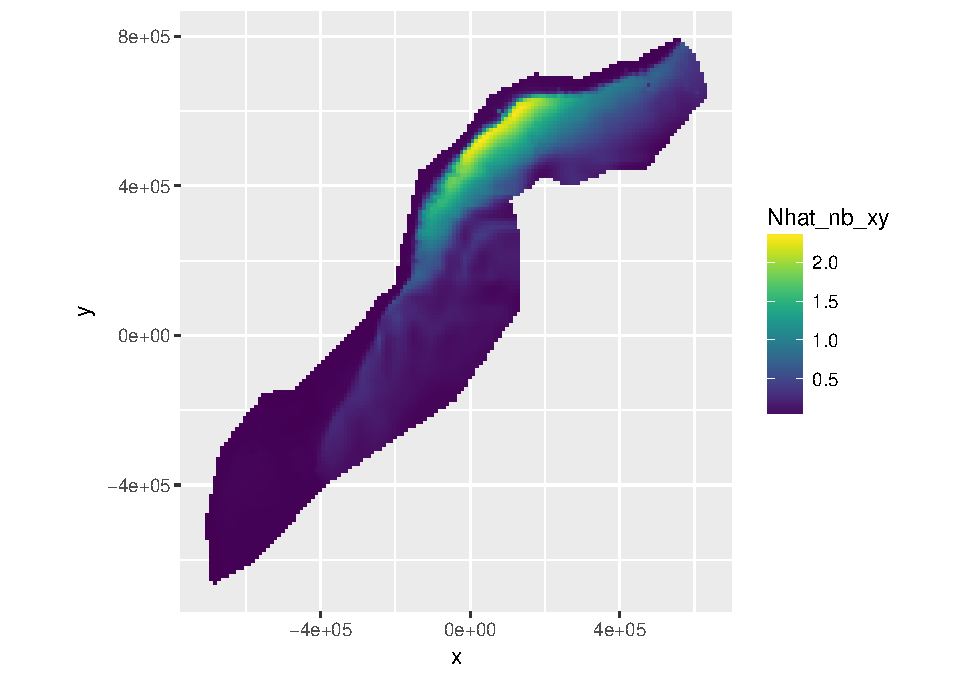
\includegraphics{_main_files/figure-latex/predsp-1.pdf}
\caption{\label{fig:predsp}Predicted surface for abundance estimates with
bivariate spatial smooth along with environmental covariates.}
\end{figure}

Copy the chunk above and make predictions for the other models you saved
in the previous exercises. In particular, compare the models with only
spatial terms to those with environmental covariates included.

\section{Save the prediction to a
raster}\label{save-the-prediction-to-a-raster}

To be able to load our predictions into ArcGIS, we need to save them as
a raster file. First we need to make our predictions into a raster
object and save them to the stack we already have:

\begin{Shaded}
\begin{Highlighting}[]
\CommentTok{# setup the storage for the predictions}
\NormalTok{pp_raster <-}\StringTok{ }\KeywordTok{raster}\NormalTok{(predictorStack)}
\CommentTok{# put the values in, making sure they are numeric first}
\NormalTok{pp_raster <-}\StringTok{ }\KeywordTok{setValues}\NormalTok{(pp_raster, }\KeywordTok{as.numeric}\NormalTok{(pp))}
\CommentTok{# name the new, last, layer in the stack}
\KeywordTok{names}\NormalTok{(pp_raster) <-}\StringTok{ "Nhat_nb_xy"}
\end{Highlighting}
\end{Shaded}

We can then save that object to disk as a raster file:

\begin{Shaded}
\begin{Highlighting}[]
\KeywordTok{writeRaster}\NormalTok{(pp_raster, }\StringTok{"abundance_raster.img"}\NormalTok{, }\DataTypeTok{datatype=}\StringTok{"FLT4S"}\NormalTok{, }\DataTypeTok{overwrite=}\OtherTok{TRUE}\NormalTok{)}
\end{Highlighting}
\end{Shaded}

Here we just saved one raster layer: the predictions from model
\texttt{Nhat\_nb\_xy}. Try saving another set of predictions from
another model by copying the above chunk.

You can check that the raster was written correctly by using the
\texttt{stack()} function, as we did before to load the data and then
the \texttt{plot()} function to see what was saved in the raster file.

\section{\texorpdfstring{Save prediction grid to
\texttt{RData}}{Save prediction grid to RData}}\label{save-prediction-grid-to-rdata}

We'll need to use the prediction grid and predictor stack again when we
calculate uncertainty in the next practical, so let's save those objects
now to save time later.

\begin{Shaded}
\begin{Highlighting}[]
\KeywordTok{save}\NormalTok{(predgrid, predictorStack, }\DataTypeTok{file=}\StringTok{"predgrid.RData"}\NormalTok{)}
\end{Highlighting}
\end{Shaded}

\section{Extra credit}\label{extra-credit-1}

\begin{itemize}
\tightlist
\item
  Try refitting your models with \texttt{family=quasipoisson()} as the
  response distribution. What do you notice about the predicted
  abundance?
\item
  Can you work out a way to use \texttt{ldply()} from the \texttt{plyr}
  package so that you can use \texttt{facet\_wrap} in \texttt{ggplot2}
  to plot predictions for multiple models in a grid layout?
\end{itemize}

\chapter{Estimating precision of predictions from density surface
models}\label{estimating-precision-of-predictions-from-density-surface-models}

Now we've fitted some models and estimated abundance, we can estimate
the variance associated with the abundance estimate (and plot it).

\section{Aims}\label{aims-5}

By the end of this practical, you should feel comfortable:

\begin{itemize}
\tightlist
\item
  Knowing when to use \texttt{dsm.var.prop} and when to use
  \texttt{dsm.var.gam}
\item
  Estimating variance for a given prediction area
\item
  Estimating variance per-cell for a prediction grid
\item
  Interpreting the \texttt{summary()} output for uncertainty estimates
\item
  Making maps of the coefficient of variation in R
\item
  Saving uncertainty information to a raster file to be read by ArcGIS
\end{itemize}

\section{Load packages and data}\label{load-packages-and-data}

\begin{Shaded}
\begin{Highlighting}[]
\KeywordTok{library}\NormalTok{(dsm)}
\KeywordTok{library}\NormalTok{(raster)}
\KeywordTok{library}\NormalTok{(ggplot2)}
\KeywordTok{library}\NormalTok{(viridis)}
\KeywordTok{library}\NormalTok{(plyr)}
\KeywordTok{library}\NormalTok{(knitr)}
\KeywordTok{library}\NormalTok{(kableExtra)}
\KeywordTok{library}\NormalTok{(rgdal)}
\end{Highlighting}
\end{Shaded}

Load the models and prediction grid:

\begin{Shaded}
\begin{Highlighting}[]
\KeywordTok{load}\NormalTok{(}\StringTok{"dsms.RData"}\NormalTok{)}
\KeywordTok{load}\NormalTok{(}\StringTok{"dsms-xy.RData"}\NormalTok{)}
\KeywordTok{load}\NormalTok{(}\StringTok{"predgrid.RData"}\NormalTok{)}
\end{Highlighting}
\end{Shaded}

\section{Estimation of variance}\label{estimation-of-variance}

Depending on the model response (count or Horvitz-Thompson) we can use
either \texttt{dsm.var.prop} or \texttt{dsm.var.gam}, respectively.
\texttt{dsm\_nb\_xy\_ms} doesn't include any covariates at the observer
level in the detection function, so we can use the variance propagation
method and estimate the uncertainty in detection function parameters in
one step.

\begin{Shaded}
\begin{Highlighting}[]
\CommentTok{# need to remove the NAs as we did when plotting}
\NormalTok{predgrid_var <-}\StringTok{ }\NormalTok{predgrid[}\OperatorTok{!}\KeywordTok{is.na}\NormalTok{(predgrid}\OperatorTok{$}\NormalTok{Depth),]}
\CommentTok{# now estimate variance}
\NormalTok{var_nb_xy_ms <-}\StringTok{ }\KeywordTok{dsm.var.prop}\NormalTok{(dsm_nb_xy_ms, predgrid_var, }
                             \DataTypeTok{off.set=}\NormalTok{predgrid_var}\OperatorTok{$}\NormalTok{off.set)}
\end{Highlighting}
\end{Shaded}

\begin{verbatim}
## Warning in dsm_varprop(dsm.obj, pred.data[[1]]): Model was fitted using
## nb() family, refitting with negbin(). See ?dsm_varprop
\end{verbatim}

To summarise the results of this variance estimate:

\begin{Shaded}
\begin{Highlighting}[]
\KeywordTok{summary}\NormalTok{(var_nb_xy_ms)}
\end{Highlighting}
\end{Shaded}

\begin{verbatim}
## Summary of uncertainty in a density surface model calculated
##  by variance propagation.
## 
## Probability of detection in fitted model and variance model
##   Fitted.model Fitted.model.se Refitted.model
## 1    0.5490484      0.03662522      0.5490484
## 
## Approximate asymptotic confidence interval:
##     2.5%     Mean    97.5% 
## 1214.633 1710.254 2408.108 
## (Using log-Normal approximation)
## 
## Point estimate                 : 1710.254 
## Standard error                 : 300.8915 
## Coefficient of variation       : 0.1759
\end{verbatim}

Try this out for some of the other models you've saved. Remember to use
\texttt{dsm.var.gam} when there are covariates in the detection function
and \texttt{dsm.var.prop} when there aren't.

\section{Summarise multiple models}\label{summarise-multiple-models}

We can again summarise all the models, as we did with the DSMs and
detection functions, now including the variance:

\begin{Shaded}
\begin{Highlighting}[]
\NormalTok{summarize_dsm_var <-}\StringTok{ }\ControlFlowTok{function}\NormalTok{(model, predgrid)\{}

\NormalTok{  summ <-}\StringTok{ }\KeywordTok{summary}\NormalTok{(model)}
  
\NormalTok{  vp <-}\StringTok{ }\KeywordTok{summary}\NormalTok{(}\KeywordTok{dsm.var.prop}\NormalTok{(model, predgrid, }\DataTypeTok{off.set=}\NormalTok{predgrid}\OperatorTok{$}\NormalTok{off.set))}
\NormalTok{  unconditional.cv.square <-}\StringTok{ }\NormalTok{vp}\OperatorTok{$}\NormalTok{cv}\OperatorTok{^}\DecValTok{2}
\NormalTok{  asymp.ci.c.term <-}\StringTok{ }\KeywordTok{exp}\NormalTok{(}\FloatTok{1.96}\OperatorTok{*}\KeywordTok{sqrt}\NormalTok{(}\KeywordTok{log}\NormalTok{(}\DecValTok{1}\OperatorTok{+}\NormalTok{unconditional.cv.square)))}
\NormalTok{  asymp.tot <-}\StringTok{ }\KeywordTok{c}\NormalTok{(vp}\OperatorTok{$}\NormalTok{pred.est }\OperatorTok{/}\StringTok{ }\NormalTok{asymp.ci.c.term,}
\NormalTok{                 vp}\OperatorTok{$}\NormalTok{pred.est,}
\NormalTok{                 vp}\OperatorTok{$}\NormalTok{pred.est }\OperatorTok{*}\StringTok{ }\NormalTok{asymp.ci.c.term)}

  \KeywordTok{data.frame}\NormalTok{(}\DataTypeTok{response =}\NormalTok{ model}\OperatorTok{$}\NormalTok{family}\OperatorTok{$}\NormalTok{family,}
             \DataTypeTok{terms    =} \KeywordTok{paste}\NormalTok{(}\KeywordTok{rownames}\NormalTok{(summ}\OperatorTok{$}\NormalTok{s.table), }\DataTypeTok{collapse=}\StringTok{", "}\NormalTok{),}
             \DataTypeTok{AIC      =} \KeywordTok{AIC}\NormalTok{(model),}
             \DataTypeTok{REML     =}\NormalTok{ model}\OperatorTok{$}\NormalTok{gcv.ubre,}
             \StringTok{"Deviance_explained"}\NormalTok{ =}\StringTok{ }\KeywordTok{paste0}\NormalTok{(}\KeywordTok{round}\NormalTok{(summ}\OperatorTok{$}\NormalTok{dev.expl}\OperatorTok{*}\DecValTok{100}\NormalTok{,}\DecValTok{2}\NormalTok{),}\StringTok{"%"}\NormalTok{),}
             \StringTok{"lower_CI"}\NormalTok{ =}\StringTok{ }\KeywordTok{round}\NormalTok{(asymp.tot[}\DecValTok{1}\NormalTok{],}\DecValTok{2}\NormalTok{),}
             \StringTok{"Nhat"}\NormalTok{ =}\StringTok{ }\KeywordTok{round}\NormalTok{(asymp.tot[}\DecValTok{2}\NormalTok{],}\DecValTok{2}\NormalTok{),}
             \StringTok{"upper_CI"}\NormalTok{ =}\StringTok{ }\KeywordTok{round}\NormalTok{(asymp.tot[}\DecValTok{3}\NormalTok{],}\DecValTok{2}\NormalTok{)}
\NormalTok{             )}
\NormalTok{\}}
\end{Highlighting}
\end{Shaded}

\begin{Shaded}
\begin{Highlighting}[]
\CommentTok{# make a list of models (add more here!)}
\NormalTok{model_list <-}\StringTok{ }\KeywordTok{list}\NormalTok{(dsm_nb_xy, dsm_nb_x_y, dsm_nb_xy_ms, dsm_nb_x_y_ms)}
\CommentTok{# give the list names for the models, so we can identify them later}
\KeywordTok{names}\NormalTok{(model_list) <-}\StringTok{ }\KeywordTok{c}\NormalTok{(}\StringTok{"dsm_nb_xy"}\NormalTok{, }\StringTok{"dsm_nb_x_y"}\NormalTok{, }\StringTok{"dsm_nb_xy_ms"}\NormalTok{, }\StringTok{"dsm_nb_x_y_ms"}\NormalTok{)}
\NormalTok{per_model_var <-}\StringTok{ }\KeywordTok{ldply}\NormalTok{(model_list, summarize_dsm_var, }\DataTypeTok{predgrid=}\NormalTok{predgrid_var)}
\end{Highlighting}
\end{Shaded}

\begin{verbatim}
## Warning in dsm_varprop(dsm.obj, pred.data[[1]]): Model was fitted using
## nb() family, refitting with negbin(). See ?dsm_varprop
\end{verbatim}

\begin{verbatim}
## Warning in newton(lsp = lsp, X = G$X, y = G$y, Eb = G$Eb, UrS = G$UrS, L =
## G$L, : Fitting terminated with step failure - check results carefully

## Warning in newton(lsp = lsp, X = G$X, y = G$y, Eb = G$Eb, UrS = G$UrS, L =
## G$L, : Fitting terminated with step failure - check results carefully

## Warning in newton(lsp = lsp, X = G$X, y = G$y, Eb = G$Eb, UrS = G$UrS, L =
## G$L, : Fitting terminated with step failure - check results carefully

## Warning in newton(lsp = lsp, X = G$X, y = G$y, Eb = G$Eb, UrS = G$UrS, L =
## G$L, : Fitting terminated with step failure - check results carefully

## Warning in newton(lsp = lsp, X = G$X, y = G$y, Eb = G$Eb, UrS = G$UrS, L =
## G$L, : Fitting terminated with step failure - check results carefully

## Warning in newton(lsp = lsp, X = G$X, y = G$y, Eb = G$Eb, UrS = G$UrS, L =
## G$L, : Fitting terminated with step failure - check results carefully

## Warning in newton(lsp = lsp, X = G$X, y = G$y, Eb = G$Eb, UrS = G$UrS, L =
## G$L, : Fitting terminated with step failure - check results carefully

## Warning in newton(lsp = lsp, X = G$X, y = G$y, Eb = G$Eb, UrS = G$UrS, L =
## G$L, : Fitting terminated with step failure - check results carefully

## Warning in newton(lsp = lsp, X = G$X, y = G$y, Eb = G$Eb, UrS = G$UrS, L =
## G$L, : Fitting terminated with step failure - check results carefully

## Warning in newton(lsp = lsp, X = G$X, y = G$y, Eb = G$Eb, UrS = G$UrS, L =
## G$L, : Fitting terminated with step failure - check results carefully

## Warning in newton(lsp = lsp, X = G$X, y = G$y, Eb = G$Eb, UrS = G$UrS, L =
## G$L, : Fitting terminated with step failure - check results carefully

## Warning in newton(lsp = lsp, X = G$X, y = G$y, Eb = G$Eb, UrS = G$UrS, L =
## G$L, : Fitting terminated with step failure - check results carefully

## Warning in newton(lsp = lsp, X = G$X, y = G$y, Eb = G$Eb, UrS = G$UrS, L =
## G$L, : Fitting terminated with step failure - check results carefully

## Warning in newton(lsp = lsp, X = G$X, y = G$y, Eb = G$Eb, UrS = G$UrS, L =
## G$L, : Fitting terminated with step failure - check results carefully

## Warning in newton(lsp = lsp, X = G$X, y = G$y, Eb = G$Eb, UrS = G$UrS, L =
## G$L, : Fitting terminated with step failure - check results carefully

## Warning in newton(lsp = lsp, X = G$X, y = G$y, Eb = G$Eb, UrS = G$UrS, L =
## G$L, : Fitting terminated with step failure - check results carefully

## Warning in newton(lsp = lsp, X = G$X, y = G$y, Eb = G$Eb, UrS = G$UrS, L =
## G$L, : Fitting terminated with step failure - check results carefully

## Warning in newton(lsp = lsp, X = G$X, y = G$y, Eb = G$Eb, UrS = G$UrS, L =
## G$L, : Fitting terminated with step failure - check results carefully

## Warning in newton(lsp = lsp, X = G$X, y = G$y, Eb = G$Eb, UrS = G$UrS, L =
## G$L, : Fitting terminated with step failure - check results carefully

## Warning in newton(lsp = lsp, X = G$X, y = G$y, Eb = G$Eb, UrS = G$UrS, L =
## G$L, : Fitting terminated with step failure - check results carefully

## Warning in newton(lsp = lsp, X = G$X, y = G$y, Eb = G$Eb, UrS = G$UrS, L =
## G$L, : Fitting terminated with step failure - check results carefully

## Warning in newton(lsp = lsp, X = G$X, y = G$y, Eb = G$Eb, UrS = G$UrS, L =
## G$L, : Fitting terminated with step failure - check results carefully

## Warning in newton(lsp = lsp, X = G$X, y = G$y, Eb = G$Eb, UrS = G$UrS, L =
## G$L, : Fitting terminated with step failure - check results carefully

## Warning in newton(lsp = lsp, X = G$X, y = G$y, Eb = G$Eb, UrS = G$UrS, L =
## G$L, : Fitting terminated with step failure - check results carefully
\end{verbatim}

\begin{verbatim}
## Warning in dsm_varprop(dsm.obj, pred.data[[1]]): Model was fitted using
## nb() family, refitting with negbin(). See ?dsm_varprop
\end{verbatim}

\begin{verbatim}
## Warning in newton(lsp = lsp, X = G$X, y = G$y, Eb = G$Eb, UrS = G$UrS, L =
## G$L, : Fitting terminated with step failure - check results carefully

## Warning in newton(lsp = lsp, X = G$X, y = G$y, Eb = G$Eb, UrS = G$UrS, L =
## G$L, : Fitting terminated with step failure - check results carefully

## Warning in newton(lsp = lsp, X = G$X, y = G$y, Eb = G$Eb, UrS = G$UrS, L =
## G$L, : Fitting terminated with step failure - check results carefully

## Warning in newton(lsp = lsp, X = G$X, y = G$y, Eb = G$Eb, UrS = G$UrS, L =
## G$L, : Fitting terminated with step failure - check results carefully

## Warning in newton(lsp = lsp, X = G$X, y = G$y, Eb = G$Eb, UrS = G$UrS, L =
## G$L, : Fitting terminated with step failure - check results carefully

## Warning in newton(lsp = lsp, X = G$X, y = G$y, Eb = G$Eb, UrS = G$UrS, L =
## G$L, : Fitting terminated with step failure - check results carefully

## Warning in newton(lsp = lsp, X = G$X, y = G$y, Eb = G$Eb, UrS = G$UrS, L =
## G$L, : Fitting terminated with step failure - check results carefully

## Warning in newton(lsp = lsp, X = G$X, y = G$y, Eb = G$Eb, UrS = G$UrS, L =
## G$L, : Fitting terminated with step failure - check results carefully

## Warning in newton(lsp = lsp, X = G$X, y = G$y, Eb = G$Eb, UrS = G$UrS, L =
## G$L, : Fitting terminated with step failure - check results carefully

## Warning in newton(lsp = lsp, X = G$X, y = G$y, Eb = G$Eb, UrS = G$UrS, L =
## G$L, : Fitting terminated with step failure - check results carefully

## Warning in newton(lsp = lsp, X = G$X, y = G$y, Eb = G$Eb, UrS = G$UrS, L =
## G$L, : Fitting terminated with step failure - check results carefully

## Warning in newton(lsp = lsp, X = G$X, y = G$y, Eb = G$Eb, UrS = G$UrS, L =
## G$L, : Fitting terminated with step failure - check results carefully

## Warning in newton(lsp = lsp, X = G$X, y = G$y, Eb = G$Eb, UrS = G$UrS, L =
## G$L, : Fitting terminated with step failure - check results carefully

## Warning in newton(lsp = lsp, X = G$X, y = G$y, Eb = G$Eb, UrS = G$UrS, L =
## G$L, : Fitting terminated with step failure - check results carefully

## Warning in newton(lsp = lsp, X = G$X, y = G$y, Eb = G$Eb, UrS = G$UrS, L =
## G$L, : Fitting terminated with step failure - check results carefully

## Warning in newton(lsp = lsp, X = G$X, y = G$y, Eb = G$Eb, UrS = G$UrS, L =
## G$L, : Fitting terminated with step failure - check results carefully

## Warning in newton(lsp = lsp, X = G$X, y = G$y, Eb = G$Eb, UrS = G$UrS, L =
## G$L, : Fitting terminated with step failure - check results carefully

## Warning in newton(lsp = lsp, X = G$X, y = G$y, Eb = G$Eb, UrS = G$UrS, L =
## G$L, : Fitting terminated with step failure - check results carefully

## Warning in newton(lsp = lsp, X = G$X, y = G$y, Eb = G$Eb, UrS = G$UrS, L =
## G$L, : Fitting terminated with step failure - check results carefully

## Warning in newton(lsp = lsp, X = G$X, y = G$y, Eb = G$Eb, UrS = G$UrS, L =
## G$L, : Fitting terminated with step failure - check results carefully

## Warning in newton(lsp = lsp, X = G$X, y = G$y, Eb = G$Eb, UrS = G$UrS, L =
## G$L, : Fitting terminated with step failure - check results carefully

## Warning in newton(lsp = lsp, X = G$X, y = G$y, Eb = G$Eb, UrS = G$UrS, L =
## G$L, : Fitting terminated with step failure - check results carefully

## Warning in newton(lsp = lsp, X = G$X, y = G$y, Eb = G$Eb, UrS = G$UrS, L =
## G$L, : Fitting terminated with step failure - check results carefully

## Warning in newton(lsp = lsp, X = G$X, y = G$y, Eb = G$Eb, UrS = G$UrS, L =
## G$L, : Fitting terminated with step failure - check results carefully
\end{verbatim}

\begin{verbatim}
## Warning in dsm_varprop(dsm.obj, pred.data[[1]]): Model was fitted using
## nb() family, refitting with negbin(). See ?dsm_varprop

## Warning in dsm_varprop(dsm.obj, pred.data[[1]]): Model was fitted using
## nb() family, refitting with negbin(). See ?dsm_varprop
\end{verbatim}

\begin{verbatim}
## Warning in newton(lsp = lsp, X = G$X, y = G$y, Eb = G$Eb, UrS = G$UrS, L =
## G$L, : Fitting terminated with step failure - check results carefully

## Warning in newton(lsp = lsp, X = G$X, y = G$y, Eb = G$Eb, UrS = G$UrS, L =
## G$L, : Fitting terminated with step failure - check results carefully

## Warning in newton(lsp = lsp, X = G$X, y = G$y, Eb = G$Eb, UrS = G$UrS, L =
## G$L, : Fitting terminated with step failure - check results carefully

## Warning in newton(lsp = lsp, X = G$X, y = G$y, Eb = G$Eb, UrS = G$UrS, L =
## G$L, : Fitting terminated with step failure - check results carefully

## Warning in newton(lsp = lsp, X = G$X, y = G$y, Eb = G$Eb, UrS = G$UrS, L =
## G$L, : Fitting terminated with step failure - check results carefully

## Warning in newton(lsp = lsp, X = G$X, y = G$y, Eb = G$Eb, UrS = G$UrS, L =
## G$L, : Fitting terminated with step failure - check results carefully

## Warning in newton(lsp = lsp, X = G$X, y = G$y, Eb = G$Eb, UrS = G$UrS, L =
## G$L, : Fitting terminated with step failure - check results carefully

## Warning in newton(lsp = lsp, X = G$X, y = G$y, Eb = G$Eb, UrS = G$UrS, L =
## G$L, : Fitting terminated with step failure - check results carefully

## Warning in newton(lsp = lsp, X = G$X, y = G$y, Eb = G$Eb, UrS = G$UrS, L =
## G$L, : Fitting terminated with step failure - check results carefully

## Warning in newton(lsp = lsp, X = G$X, y = G$y, Eb = G$Eb, UrS = G$UrS, L =
## G$L, : Fitting terminated with step failure - check results carefully

## Warning in newton(lsp = lsp, X = G$X, y = G$y, Eb = G$Eb, UrS = G$UrS, L =
## G$L, : Fitting terminated with step failure - check results carefully

## Warning in newton(lsp = lsp, X = G$X, y = G$y, Eb = G$Eb, UrS = G$UrS, L =
## G$L, : Fitting terminated with step failure - check results carefully

## Warning in newton(lsp = lsp, X = G$X, y = G$y, Eb = G$Eb, UrS = G$UrS, L =
## G$L, : Fitting terminated with step failure - check results carefully

## Warning in newton(lsp = lsp, X = G$X, y = G$y, Eb = G$Eb, UrS = G$UrS, L =
## G$L, : Fitting terminated with step failure - check results carefully

## Warning in newton(lsp = lsp, X = G$X, y = G$y, Eb = G$Eb, UrS = G$UrS, L =
## G$L, : Fitting terminated with step failure - check results carefully

## Warning in newton(lsp = lsp, X = G$X, y = G$y, Eb = G$Eb, UrS = G$UrS, L =
## G$L, : Fitting terminated with step failure - check results carefully

## Warning in newton(lsp = lsp, X = G$X, y = G$y, Eb = G$Eb, UrS = G$UrS, L =
## G$L, : Fitting terminated with step failure - check results carefully

## Warning in newton(lsp = lsp, X = G$X, y = G$y, Eb = G$Eb, UrS = G$UrS, L =
## G$L, : Fitting terminated with step failure - check results carefully

## Warning in newton(lsp = lsp, X = G$X, y = G$y, Eb = G$Eb, UrS = G$UrS, L =
## G$L, : Fitting terminated with step failure - check results carefully

## Warning in newton(lsp = lsp, X = G$X, y = G$y, Eb = G$Eb, UrS = G$UrS, L =
## G$L, : Fitting terminated with step failure - check results carefully

## Warning in newton(lsp = lsp, X = G$X, y = G$y, Eb = G$Eb, UrS = G$UrS, L =
## G$L, : Fitting terminated with step failure - check results carefully

## Warning in newton(lsp = lsp, X = G$X, y = G$y, Eb = G$Eb, UrS = G$UrS, L =
## G$L, : Fitting terminated with step failure - check results carefully
\end{verbatim}

\begin{Shaded}
\begin{Highlighting}[]
\KeywordTok{kable}\NormalTok{(per_model_var, }\DataTypeTok{digits=}\DecValTok{1}\NormalTok{, }\DataTypeTok{booktabs=}\OtherTok{TRUE}\NormalTok{, }\DataTypeTok{escape=}\OtherTok{TRUE}\NormalTok{, }
      \DataTypeTok{caption =} \StringTok{"Model performance: bivariate vs univariate spatial smooths without and with environmental covariates."}\NormalTok{) }\OperatorTok
\StringTok{  }\KeywordTok{kable_styling}\NormalTok{(}\DataTypeTok{latex_options=}\StringTok{"scale_down"}\NormalTok{)}
\end{Highlighting}
\end{Shaded}

\begin{table}

\caption{\label{tab:print-table}Model performance: bivariate vs univariate spatial smooths without and with environmental covariates.}
\centering
\resizebox{\linewidth}{!}{\begin{tabular}[t]{lllrrlrrr}
\toprule
.id & response & terms & AIC & REML & Deviance\_explained & lower\_CI & Nhat & upper\_CI\\
\midrule
dsm\_nb\_xy & Negative Binomial(0.105) & s(x,y) & 775.3 & 392.6 & 40.65\% & 1026.8 & 1661.6 & 2688.8\\
dsm\_nb\_x\_y & Negative Binomial(0.085) & s(x), s(y) & 789.8 & 395.9 & 31.14\% & 1067.0 & 1584.0 & 2351.4\\
dsm\_nb\_xy\_ms & Negative Binomial(0.114) & s(x,y), s(Depth), s(DistToCAS), s(SST), s(EKE), s(NPP) & 754.0 & 382.8 & 39.2\% & 1214.6 & 1710.2 & 2408.1\\
dsm\_nb\_x\_y\_ms & Negative Binomial(0.116) & s(x), s(y), s(Depth), s(DistToCAS), s(SST), s(EKE), s(NPP) & 752.6 & 383.0 & 40.73\% & 770.8 & 1348.4 & 2359.0\\
\bottomrule
\end{tabular}}
\end{table}

\section{Plotting}\label{plotting-1}

We can plot a map of the coefficient of variation, but we first need to
estimate the variance per prediction cell, rather than over the whole
area. This calculation takes a while!

\begin{Shaded}
\begin{Highlighting}[]
\CommentTok{# use the split function to make each row of the predictiond data.frame into}
\CommentTok{# an element of a list}
\NormalTok{predgrid_var_split <-}\StringTok{ }\KeywordTok{split}\NormalTok{(predgrid_var, }\DecValTok{1}\OperatorTok{:}\KeywordTok{nrow}\NormalTok{(predgrid_var))}
\NormalTok{var_split_nb_xy_ms <-}\StringTok{ }\KeywordTok{dsm.var.prop}\NormalTok{(dsm_nb_xy_ms, predgrid_var_split, }
                                   \DataTypeTok{off.set=}\NormalTok{predgrid_var}\OperatorTok{$}\NormalTok{off.set)}
\end{Highlighting}
\end{Shaded}

\begin{verbatim}
## Warning in dsm_varprop(dsm.obj, pred.data[[1]]): Model was fitted using
## nb() family, refitting with negbin(). See ?dsm_varprop
\end{verbatim}

Now we have the per-cell coefficients of variation, we assign that to a
column of the prediction grid data and plot it as usual:

\begin{Shaded}
\begin{Highlighting}[]
\NormalTok{predgrid_var_map <-}\StringTok{ }\NormalTok{predgrid_var}
\NormalTok{cv <-}\StringTok{ }\KeywordTok{sqrt}\NormalTok{(var_split_nb_xy_ms}\OperatorTok{$}\NormalTok{pred.var)}\OperatorTok{/}\KeywordTok{unlist}\NormalTok{(var_split_nb_xy_ms}\OperatorTok{$}\NormalTok{pred)}
\NormalTok{predgrid_var_map}\OperatorTok{$}\NormalTok{CV <-}\StringTok{ }\NormalTok{cv}
\NormalTok{p <-}\StringTok{ }\KeywordTok{ggplot}\NormalTok{(predgrid_var_map) }\OperatorTok{+}
\StringTok{       }\KeywordTok{geom_tile}\NormalTok{(}\KeywordTok{aes}\NormalTok{(}\DataTypeTok{x=}\NormalTok{x, }\DataTypeTok{y=}\NormalTok{y, }\DataTypeTok{fill=}\NormalTok{CV, }\DataTypeTok{width=}\DecValTok{10}\OperatorTok{*}\DecValTok{1000}\NormalTok{, }\DataTypeTok{height=}\DecValTok{10}\OperatorTok{*}\DecValTok{1000}\NormalTok{)) }\OperatorTok{+}
\StringTok{       }\KeywordTok{scale_fill_viridis}\NormalTok{() }\OperatorTok{+}
\StringTok{       }\KeywordTok{coord_equal}\NormalTok{() }\OperatorTok{+}
\StringTok{       }\KeywordTok{geom_point}\NormalTok{(}\KeywordTok{aes}\NormalTok{(}\DataTypeTok{x=}\NormalTok{x,}\DataTypeTok{y=}\NormalTok{y, }\DataTypeTok{size=}\NormalTok{count), }
                  \DataTypeTok{data=}\NormalTok{dsm_nb_xy_ms}\OperatorTok{$}\NormalTok{data[dsm_nb_xy_ms}\OperatorTok{$}\NormalTok{data}\OperatorTok{$}\NormalTok{count}\OperatorTok{>}\DecValTok{0}\NormalTok{,])}
\end{Highlighting}
\end{Shaded}

\begin{verbatim}
## Warning: Ignoring unknown aesthetics: width, height
\end{verbatim}

\begin{Shaded}
\begin{Highlighting}[]
\KeywordTok{print}\NormalTok{(p)}
\end{Highlighting}
\end{Shaded}

\begin{figure}
\centering
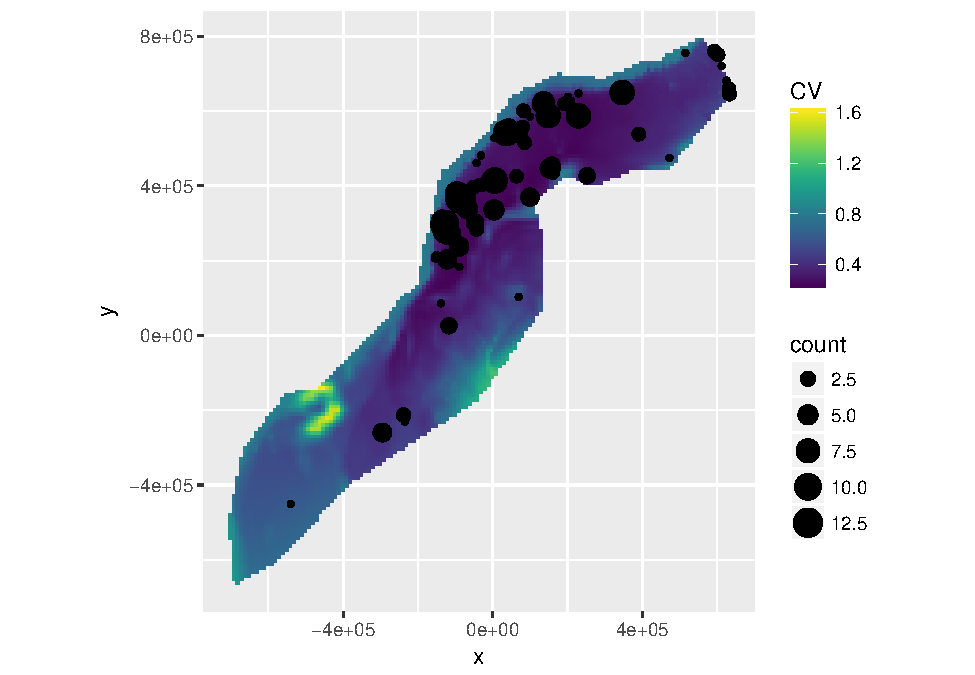
\includegraphics{_main_files/figure-latex/varest-map-obs-1.pdf}
\caption{\label{fig:varest-map-obs}Uncertainty (CV) in prediction surface
from bivariate spatial smooth with environmental covariates. Sightings
overlaid.}
\end{figure}

Note that here we overplot the segments where sperm whales were observed
(and scale the size of the point according to the number observed),
using \texttt{geom\_point()}.

We can also overplot the effort, which can be a useful way to see what
the cause of uncertainty is. Though it may not only be caused by lack of
effort but also covariate coverage, this can be useful to see.

First we need to load the segment data from the \texttt{gdb}

\begin{Shaded}
\begin{Highlighting}[]
\NormalTok{tracks <-}\StringTok{ }\KeywordTok{readOGR}\NormalTok{(}\StringTok{"Analysis.gdb"}\NormalTok{, }\StringTok{"Segments"}\NormalTok{)}
\end{Highlighting}
\end{Shaded}

\begin{verbatim}
## OGR data source with driver: OpenFileGDB 
## Source: "Analysis.gdb", layer: "Segments"
## with 949 features
## It has 8 fields
\end{verbatim}

\begin{Shaded}
\begin{Highlighting}[]
\NormalTok{tracks <-}\StringTok{ }\KeywordTok{fortify}\NormalTok{(tracks)}
\end{Highlighting}
\end{Shaded}

We can then just add this to the plot object we have built so far (with
\texttt{+}), but this looks a bit messy with the observations, so let's
start from scratch:

\begin{Shaded}
\begin{Highlighting}[]
\NormalTok{p <-}\StringTok{ }\KeywordTok{ggplot}\NormalTok{(predgrid_var_map) }\OperatorTok{+}
\StringTok{       }\KeywordTok{geom_tile}\NormalTok{(}\KeywordTok{aes}\NormalTok{(}\DataTypeTok{x=}\NormalTok{x, }\DataTypeTok{y=}\NormalTok{y, }\DataTypeTok{fill=}\NormalTok{CV, }\DataTypeTok{width=}\DecValTok{10}\OperatorTok{*}\DecValTok{1000}\NormalTok{, }\DataTypeTok{height=}\DecValTok{10}\OperatorTok{*}\DecValTok{1000}\NormalTok{)) }\OperatorTok{+}
\StringTok{       }\KeywordTok{scale_fill_viridis}\NormalTok{() }\OperatorTok{+}
\StringTok{       }\KeywordTok{coord_equal}\NormalTok{() }\OperatorTok{+}
\StringTok{       }\KeywordTok{geom_path}\NormalTok{(}\KeywordTok{aes}\NormalTok{(}\DataTypeTok{x=}\NormalTok{long, }\DataTypeTok{y=}\NormalTok{lat, }\DataTypeTok{group=}\NormalTok{group), }\DataTypeTok{data=}\NormalTok{tracks)}
\end{Highlighting}
\end{Shaded}

\begin{verbatim}
## Warning: Ignoring unknown aesthetics: width, height
\end{verbatim}

\begin{Shaded}
\begin{Highlighting}[]
\KeywordTok{print}\NormalTok{(p)}
\end{Highlighting}
\end{Shaded}

\begin{figure}
\centering
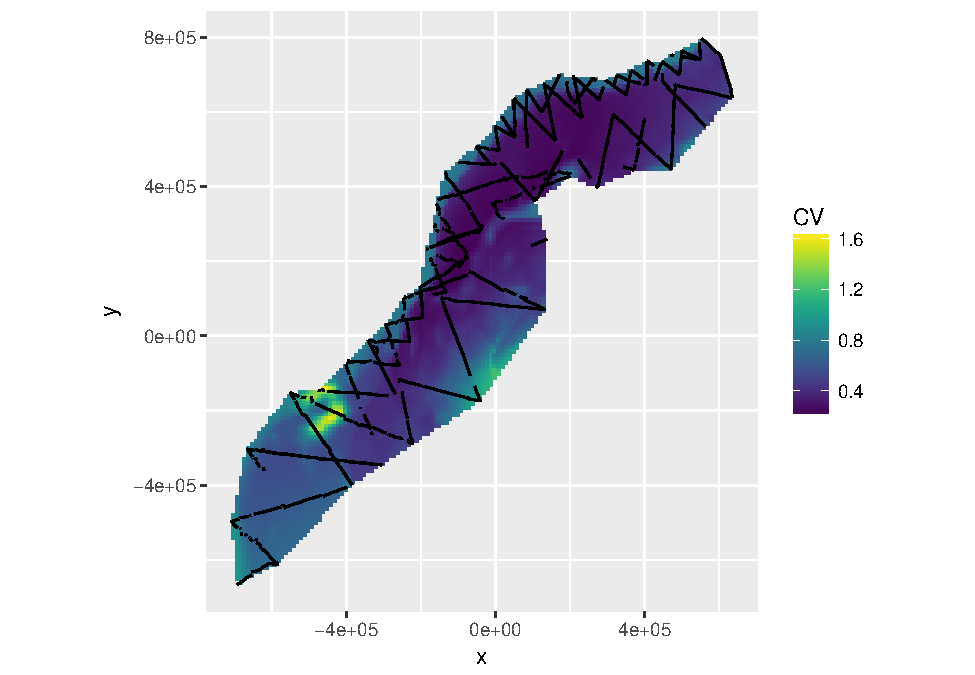
\includegraphics{_main_files/figure-latex/varest-map-obs-effort-1.pdf}
\caption{\label{fig:varest-map-obs-effort}Uncertainty (CV) in prediction
surface from bivariate spatial smooth with environmental covariates.
Effort overlaid.}
\end{figure}

Try this with the other models you fitted and see what the differences
are between the maps of coefficient of variation.

\section{Save the uncertainty maps to raster
files}\label{save-the-uncertainty-maps-to-raster-files}

As with the predictions, we'd like to save our uncertainty estimates to
a raster layer so we can plot them in ArcGIS. Again, this involves a bit
of messing about with the data format before we can save.

\begin{Shaded}
\begin{Highlighting}[]
\CommentTok{# setup the storage for the cvs}
\NormalTok{cv_raster <-}\StringTok{ }\KeywordTok{raster}\NormalTok{(predictorStack)}
\CommentTok{# we removed the NA values to make the predictions and the raster needs them}
\CommentTok{# so make a vector of NAs, and insert the CV values...}
\NormalTok{cv_na <-}\StringTok{ }\KeywordTok{rep}\NormalTok{(}\OtherTok{NA}\NormalTok{, }\KeywordTok{nrow}\NormalTok{(predgrid))}
\NormalTok{cv_na[}\OperatorTok{!}\KeywordTok{is.na}\NormalTok{(predgrid}\OperatorTok{$}\NormalTok{Depth)] <-}\StringTok{ }\NormalTok{cv}
\CommentTok{# put the values in, making sure they are numeric first}
\NormalTok{cv_raster <-}\StringTok{ }\KeywordTok{setValues}\NormalTok{(cv_raster, cv_na)}
\CommentTok{# name the new, last, layer in the stack}
\KeywordTok{names}\NormalTok{(cv_raster) <-}\StringTok{ "CV_nb_xy"}
\end{Highlighting}
\end{Shaded}

We can then save that object to disk as a raster file:

\begin{Shaded}
\begin{Highlighting}[]
\KeywordTok{writeRaster}\NormalTok{(cv_raster, }\StringTok{"cv_raster.img"}\NormalTok{, }\DataTypeTok{datatype=}\StringTok{"FLT4S"}\NormalTok{, }\DataTypeTok{overwrite=}\OtherTok{TRUE}\NormalTok{)}
\end{Highlighting}
\end{Shaded}

\section{Extra credit}\label{extra-credit-2}

\begin{itemize}
\tightlist
\item
  \texttt{dsm.var.prop} and \texttt{dsm.var.gam} can accept arbitrary
  splits in the data, not just whole areas or cells. Make a
  \texttt{list} with two elements: one a \texttt{data.frame} of all the
  cells with \(y>0\) and one with \(y\leq 0\). Estimate the variance for
  these regions. Note that you'll need to sum the offsets for each area
  to get the correct value to supply to \texttt{off.set=...}.
\end{itemize}

\chapter{Mark-recapture distance sampling of
golftees}\label{mark-recapture-distance-sampling-of-golftees}

This document is designed to give you some pointers so that you can
perform the Mark-Recapture Distance Sampling practical directly using
the \texttt{mrds} package in R, rather than via the Distance graphical
interface. I assume you have some knowledge of R, the \texttt{mrds}
package, and Distance.

\section{Golf tee survey}\label{golf-tee-survey}

Luckily for us, the golf tee dataset is provided aspart of the mrds
package, so we don't have to worry about obtaining the data from the
Distance GolfteesExercise project.

Open R and load the mrds library and golf tee dataset.

\begin{Shaded}
\begin{Highlighting}[]
\KeywordTok{library}\NormalTok{(mrds)}
\KeywordTok{data}\NormalTok{(book.tee.data)}
\CommentTok{#investigate the structure of the dataset}
\KeywordTok{str}\NormalTok{(book.tee.data)}
\end{Highlighting}
\end{Shaded}

\begin{verbatim}
List of 4
 $ book.tee.dataframe:'data.frame': 324 obs. of  7 variables:
  ..$ object  : num [1:324] 1 1 2 2 3 3 4 4 5 5 ...
  ..$ observer: Factor w/ 2 levels "1","2": 1 2 1 2 1 2 1 2 1 2 ...
  ..$ detected: num [1:324] 1 0 1 0 1 0 1 0 1 0 ...
  ..$ distance: num [1:324] 2.68 2.68 3.33 3.33 0.34 0.34 2.53 2.53 1.46 1.46 ...
  ..$ size    : num [1:324] 2 2 2 2 1 1 2 2 2 2 ...
  ..$ sex     : num [1:324] 1 1 1 1 0 0 1 1 1 1 ...
  ..$ exposure: num [1:324] 1 1 0 0 0 0 1 1 0 0 ...
 $ book.tee.region   :'data.frame': 2 obs. of  2 variables:
  ..$ Region.Label: Factor w/ 2 levels "1","2": 1 2
  ..$ Area        : num [1:2] 1040 640
 $ book.tee.samples  :'data.frame': 11 obs. of  3 variables:
  ..$ Sample.Label: num [1:11] 1 2 3 4 5 6 7 8 9 10 ...
  ..$ Region.Label: Factor w/ 2 levels "1","2": 1 1 1 1 1 1 2 2 2 2 ...
  ..$ Effort      : num [1:11] 10 30 30 27 21 12 23 23 15 12 ...
 $ book.tee.obs      :'data.frame': 162 obs. of  3 variables:
  ..$ object      : int [1:162] 1 2 3 21 22 23 24 59 60 61 ...
  ..$ Region.Label: int [1:162] 1 1 1 1 1 1 1 1 1 1 ...
  ..$ Sample.Label: int [1:162] 1 1 1 1 1 1 1 1 1 1 ...
\end{verbatim}

\begin{Shaded}
\begin{Highlighting}[]
\CommentTok{#extract the list elements from the dataset into easy-to-use objects}
\NormalTok{detections <-}\StringTok{ }\NormalTok{book.tee.data}\OperatorTok{$}\NormalTok{book.tee.dataframe}
\CommentTok{#make sure sex and exposure are factor variables}
\NormalTok{detections}\OperatorTok{$}\NormalTok{sex <-}\StringTok{ }\KeywordTok{as.factor}\NormalTok{(detections}\OperatorTok{$}\NormalTok{sex)}
\NormalTok{detections}\OperatorTok{$}\NormalTok{exposure <-}\StringTok{ }\KeywordTok{as.factor}\NormalTok{(detections}\OperatorTok{$}\NormalTok{exposure)}
\NormalTok{region <-}\StringTok{ }\NormalTok{book.tee.data}\OperatorTok{$}\NormalTok{book.tee.region}
\NormalTok{samples <-}\StringTok{ }\NormalTok{book.tee.data}\OperatorTok{$}\NormalTok{book.tee.samples}
\NormalTok{obs <-}\StringTok{ }\NormalTok{book.tee.data}\OperatorTok{$}\NormalTok{book.tee.obs}
\end{Highlighting}
\end{Shaded}

We'll start by fitting the initial full independence model, with only
distance as a covariate - just as was done in the ``FI - MR dist'' model
in Distance. Indeed, if you did fit that model in Distance, you can look
in the Log tab at the R code Distance generated, and compare it with the
code we use here.

Feel free to use \texttt{?} to find out more about any of the functions
used -- e.g., \texttt{?ddf} will tell you more about the ddf function.

\begin{Shaded}
\begin{Highlighting}[]
\CommentTok{#Fit the model}
\NormalTok{fi.mr.dist <-}\StringTok{ }\KeywordTok{ddf}\NormalTok{(}\DataTypeTok{method=}\StringTok{'trial.fi'}\NormalTok{,}\DataTypeTok{mrmodel=}\OperatorTok{~}\KeywordTok{glm}\NormalTok{(}\DataTypeTok{link=}\StringTok{'logit'}\NormalTok{,}\DataTypeTok{formula=}\OperatorTok{~}\NormalTok{distance),}
                \DataTypeTok{data=}\NormalTok{detections,}\DataTypeTok{meta.data=}\KeywordTok{list}\NormalTok{(}\DataTypeTok{width=}\DecValTok{4}\NormalTok{))}
\CommentTok{#Create a set of tables summarizing the double observer data (this is what Distance does)}
\NormalTok{detection.tables <-}\StringTok{ }\KeywordTok{det.tables}\NormalTok{(fi.mr.dist)}
\CommentTok{#Print these detection tables}
\NormalTok{detection.tables}
\end{Highlighting}
\end{Shaded}

\begin{verbatim}

Observer 1 detections
           Detected
            Missed Detected
  [0,0.4]        1       25
  (0.4,0.8]      2       16
  (0.8,1.2]      2       16
  (1.2,1.6]      6       22
  (1.6,2]        5        9
  (2,2.4]        2       10
  (2.4,2.8]      6       12
  (2.8,3.2]      6        9
  (3.2,3.6]      2        3
  (3.6,4]        6        2

Observer 2 detections
           Detected
            Missed Detected
  [0,0.4]        4       22
  (0.4,0.8]      1       17
  (0.8,1.2]      0       18
  (1.2,1.6]      2       26
  (1.6,2]        1       13
  (2,2.4]        2       10
  (2.4,2.8]      3       15
  (2.8,3.2]      4       11
  (3.2,3.6]      2        3
  (3.6,4]        1        7

Duplicate detections

  [0,0.4] (0.4,0.8] (0.8,1.2] (1.2,1.6]   (1.6,2]   (2,2.4] (2.4,2.8] 
       21        15        16        20         8         8         9 
(2.8,3.2] (3.2,3.6]   (3.6,4] 
        5         1         1 

Observer 1 detections of those seen by Observer 2
          Missed Detected Prop. detected
[0,0.4]        1       21      0.9545455
(0.4,0.8]      2       15      0.8823529
(0.8,1.2]      2       16      0.8888889
(1.2,1.6]      6       20      0.7692308
(1.6,2]        5        8      0.6153846
(2,2.4]        2        8      0.8000000
(2.4,2.8]      6        9      0.6000000
(2.8,3.2]      6        5      0.4545455
(3.2,3.6]      2        1      0.3333333
(3.6,4]        6        1      0.1428571
\end{verbatim}

\begin{Shaded}
\begin{Highlighting}[]
\CommentTok{# They could also be plotted, but I've not done so in the interest of space}
\CommentTok{# plot(detection.tables)}

\CommentTok{#Produce a summary of the fitted detection function object}
\KeywordTok{summary}\NormalTok{(fi.mr.dist)}
\end{Highlighting}
\end{Shaded}

\begin{verbatim}

Summary for trial.fi object 
Number of observations               :  162 
Number seen by primary               :  124 
Number seen by secondary (trials)    :  142 
Number seen by both (detected trials):  104 
AIC                                  :  452.8094 


Conditional detection function parameters:
             estimate        se
(Intercept)  2.900233 0.4876238
distance    -1.058677 0.2235722

                        Estimate          SE         CV
Average p              0.6423252  0.04069409 0.06335434
Average primary p(0)   0.9478579  0.06109655 0.06445750
N in covered region  193.0486185 15.84826458 0.08209468
\end{verbatim}

\begin{Shaded}
\begin{Highlighting}[]
\CommentTok{#Produce goodness of fit statistics and a qq plot}
\NormalTok{gof.result <-}\StringTok{ }\KeywordTok{ddf.gof}\NormalTok{(fi.mr.dist, }
                      \DataTypeTok{main=}\StringTok{"Full independence, trial mode goodness of fit}\CharTok{\textbackslash{}n}\StringTok{Golftee data"}\NormalTok{)}
\end{Highlighting}
\end{Shaded}

\begin{figure}
\centering
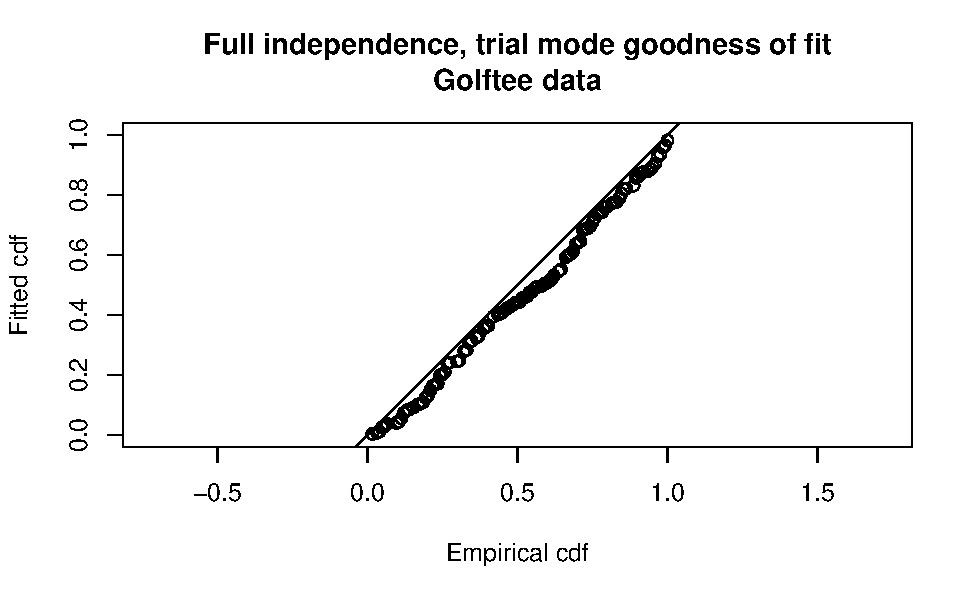
\includegraphics{_main_files/figure-latex/fit-nocovar-1.pdf}
\caption{\label{fig:fit-nocovar}Goodness of fit (FI-trial) to golftee data.}
\end{figure}

\begin{Shaded}
\begin{Highlighting}[]
\NormalTok{chi.distance <-}\StringTok{ }\NormalTok{gof.result}\OperatorTok{$}\NormalTok{chisquare}\OperatorTok{$}\NormalTok{chi1}\OperatorTok{$}\NormalTok{chisq}
\NormalTok{chi.markrecap <-}\StringTok{ }\NormalTok{gof.result}\OperatorTok{$}\NormalTok{chisquare}\OperatorTok{$}\NormalTok{chi2}\OperatorTok{$}\NormalTok{chisq}
\NormalTok{chi.total <-}\StringTok{ }\NormalTok{gof.result}\OperatorTok{$}\NormalTok{chisquare}\OperatorTok{$}\NormalTok{pooled.chi}
\end{Highlighting}
\end{Shaded}

Abbreviated \(\chi^2\) goodness of fit assessment shows the \(\chi^2\)
contribution from the distance sampling model to be 11.5 and the
\(\chi^2\) contribution from the mark-recapture model to be 3.4. The
combination of these elements produces a total \(\chi^2\) of 14.9 with
17 degrees of freedom, resulting in a P-value of 0.604

\begin{Shaded}
\begin{Highlighting}[]
\CommentTok{#Calculate density estimates using the dht function}
\NormalTok{tee.abund <-}\StringTok{ }\KeywordTok{dht}\NormalTok{(fi.mr.dist,region,samples,obs)}
\KeywordTok{kable}\NormalTok{(tee.abund}\OperatorTok{$}\NormalTok{individuals}\OperatorTok{$}\NormalTok{summary, }\DataTypeTok{digits=}\DecValTok{2}\NormalTok{, }
      \DataTypeTok{caption=}\StringTok{"Survey summary statistics for golftees"}\NormalTok{)}
\end{Highlighting}
\end{Shaded}

\begin{table}

\caption{\label{tab:abund-from-dist}Survey summary statistics for golftees}
\centering
\begin{tabular}[t]{l|r|r|r|r|r|r|r|r|r}
\hline
Region & Area & CoveredArea & Effort & n & ER & se.ER & cv.ER & mean.size & se.mean\\
\hline
1 & 1040 & 1040 & 130 & 229 & 1.76 & 0.12 & 0.07 & 3.18 & 0.21\\
\hline
2 & 640 & 640 & 80 & 152 & 1.90 & 0.33 & 0.18 & 2.92 & 0.23\\
\hline
Total & 1680 & 1680 & 210 & 381 & 1.81 & 0.14 & 0.08 & 3.07 & 0.15\\
\hline
\end{tabular}
\end{table}

\begin{Shaded}
\begin{Highlighting}[]
\KeywordTok{kable}\NormalTok{(tee.abund}\OperatorTok{$}\NormalTok{individuals}\OperatorTok{$}\NormalTok{N, }\DataTypeTok{digits=}\DecValTok{2}\NormalTok{, }
      \DataTypeTok{caption=}\StringTok{"Abundance estimates for golftee population with two strata"}\NormalTok{)}
\end{Highlighting}
\end{Shaded}

\begin{table}

\caption{\label{tab:abund-from-dist}Abundance estimates for golftee population with two strata}
\centering
\begin{tabular}[t]{l|r|r|r|r|r|r}
\hline
Label & Estimate & se & cv & lcl & ucl & df\\
\hline
1 & 356.52 & 32.35 & 0.09 & 294.54 & 431.53 & 17.13\\
\hline
2 & 236.64 & 44.14 & 0.19 & 147.33 & 380.09 & 5.06\\
\hline
Total & 593.16 & 60.38 & 0.10 & 478.32 & 735.57 & 16.06\\
\hline
\end{tabular}
\end{table}

Now, see if you can work out how to change the call to ddf to fit the
other models mentioned in the exercise, and then write code to enable
you to compare the models and select among them.

\section{Crabeater seal survey}\label{crabeater-seal-survey}

This analysis is described in Borchers et al.
(\protect\hyperlink{ref-Borchers_2005}{2005}) Biometrics paper of aerial
survey data looking for seals in the Antarctic pack ice. There were four
observers in the plane, two on each side (front and back).

The data from the survey has been saved in a \texttt{.csv} file. This
file can be easily read into R, and with the \texttt{checkdata()}
function, the information to construct the region, sample, and
observation table can be extracted. Note that these tables are only
needed when estimating abundance by scaling up from the covered region
to the study area.

\begin{Shaded}
\begin{Highlighting}[]
\KeywordTok{library}\NormalTok{(Distance)}
\NormalTok{crabseal <-}\StringTok{ }\KeywordTok{read.csv}\NormalTok{(}\StringTok{"crabbieMRDS.csv"}\NormalTok{)}
\CommentTok{#  Half normal detection function, 700m truncation distance, }
\CommentTok{#      logit function for mark-recapture component}
\NormalTok{crab.ddf.io <-}\StringTok{ }\KeywordTok{ddf}\NormalTok{(}\DataTypeTok{method=}\StringTok{"io"}\NormalTok{, }\DataTypeTok{dsmodel=}\OperatorTok{~}\KeywordTok{cds}\NormalTok{(}\DataTypeTok{key=}\StringTok{"hn"}\NormalTok{),}
                 \DataTypeTok{mrmodel=}\OperatorTok{~}\KeywordTok{glm}\NormalTok{(}\DataTypeTok{link=}\StringTok{"logit"}\NormalTok{, }\DataTypeTok{formula=}\OperatorTok{~}\NormalTok{distance),}
                 \DataTypeTok{data=}\NormalTok{crabseal, }\DataTypeTok{meta.data=}\KeywordTok{list}\NormalTok{(}\DataTypeTok{width=}\DecValTok{700}\NormalTok{))}
\KeywordTok{summary}\NormalTok{(crab.ddf.io)}
\end{Highlighting}
\end{Shaded}

\begin{verbatim}

Summary for io.fi object 
Number of observations   :  1740 
Number seen by primary   :  1394 
Number seen by secondary :  1471 
Number seen by both      :  1125 
AIC                      :  3011.463 


Conditional detection function parameters:
                estimate           se
(Intercept)  2.107762345 0.0994391200
distance    -0.003087713 0.0003159216

                        Estimate          SE          CV
Average primary p(0)   0.8916554 0.009606428 0.010773701
Average secondary p(0) 0.8916554 0.009606428 0.010773701
Average combined p(0)  0.9882614 0.002081614 0.002106339


Summary for ds object 
Number of observations :  1740 
Distance range         :  0  -  700 
AIC                    :  22314.4 

Detection function:
 Half-normal key function 

Detection function parameters 
Scale coefficient(s):  
            estimate        se
(Intercept) 5.828703 0.0268578

           Estimate         SE         CV
Average p 0.5845871 0.01247837 0.02134562


Summary for io object
Total AIC value :  25325.86 

                        Estimate          SE         CV
Average p              0.5777249  0.01239179 0.02144929
N in covered region 3011.8139211 79.84197966 0.02650960
\end{verbatim}

Goodness of fit could be examined in the same manner as the golf tees by
the use of \texttt{ddf.gof(crab.ddf.io)} but I have not shown this step.

Following model criticism and selection, estimation of abundance ensues.
the estimates of abundance for the study area are arbitrary because
inference of the study was restricted to the covered region. Hence the
estimates of abundance here are artificial, but if we wished to produce
them, we would need to produce the region, sample, and observation
tables and apply Horvitz-Thompson like estimators to produce estimates
of \(\hat{N}\). The use of \texttt{covert.units} adjusts the units of
perpendicular distance measurement (m) to units of transect effort (km).
Be sure to perform the conversion correctly or your abundance estimates
will be off by orders of magnitude.

\begin{Shaded}
\begin{Highlighting}[]
\NormalTok{tables <-}\StringTok{ }\NormalTok{Distance}\OperatorTok{:::}\KeywordTok{checkdata}\NormalTok{(crabseal[crabseal}\OperatorTok{$}\NormalTok{observer}\OperatorTok{==}\DecValTok{1}\NormalTok{,])}
\NormalTok{crab.ddf.io.abund <-}\StringTok{ }\KeywordTok{dht}\NormalTok{(}\DataTypeTok{region=}\NormalTok{tables}\OperatorTok{$}\NormalTok{region.table, }
                         \DataTypeTok{sample=}\NormalTok{tables}\OperatorTok{$}\NormalTok{sample.table, }\DataTypeTok{obs=}\NormalTok{tables}\OperatorTok{$}\NormalTok{obs.table,}
                         \DataTypeTok{model=}\NormalTok{crab.ddf.io, }\DataTypeTok{se=}\OtherTok{TRUE}\NormalTok{, }\DataTypeTok{options=}\KeywordTok{list}\NormalTok{(}\DataTypeTok{convert.units=}\FloatTok{0.001}\NormalTok{))}
\KeywordTok{kable}\NormalTok{(crab.ddf.io.abund}\OperatorTok{$}\NormalTok{individuals}\OperatorTok{$}\NormalTok{summary, }\DataTypeTok{digits=}\DecValTok{3}\NormalTok{,}
      \DataTypeTok{caption=}\StringTok{"Summary information from crabeater seal aerial survey."}\NormalTok{)}
\end{Highlighting}
\end{Shaded}

\begin{table}

\caption{\label{tab:crabsummary}Summary information from crabeater seal aerial survey.}
\centering
\begin{tabular}[t]{l|r|r|r|r|r|r|r|r|r}
\hline
Region & Area & CoveredArea & Effort & n & ER & se.ER & cv.ER & mean.size & se.mean\\
\hline
1 & 1e+06 & 8594.082 & 6138.63 & 2053 & 0.334 & 0.033 & 0.097 & 1.18 & 0.013\\
\hline
\end{tabular}
\end{table}

\begin{Shaded}
\begin{Highlighting}[]
\KeywordTok{kable}\NormalTok{(crab.ddf.io.abund}\OperatorTok{$}\NormalTok{individual}\OperatorTok{$}\NormalTok{N, }\DataTypeTok{digits=}\DecValTok{3}\NormalTok{,}
      \DataTypeTok{caption=}\StringTok{"Crabeater seal abundance estimates for study area of arbitrary size."}\NormalTok{)}
\end{Highlighting}
\end{Shaded}

\begin{table}

\caption{\label{tab:crabestimates}Crabeater seal abundance estimates for study area of arbitrary size.}
\centering
\begin{tabular}[t]{l|r|r|r|r|r|r}
\hline
Label & Estimate & se & cv & lcl & ucl & df\\
\hline
Total & 413493.2 & 41201.49 & 0.09964248 & 339670.9 & 503359.6 & 128.6257\\
\hline
\end{tabular}
\end{table}

\chapter*{References}\label{references}
\addcontentsline{toc}{chapter}{References}

\hypertarget{refs}{}
\hypertarget{ref-Amodio2014}{}
Amodio, Sonia, Massimo Aria, and Antonio D'Ambrosio. 2014. ``On
Concurvity in Nonlinear and Nonparametric Regression Models.''
\emph{Statistica} 74 (1): 85--98.
doi:\href{https://doi.org/10.6092/issn.1973-2201/4599}{10.6092/issn.1973-2201/4599}.

\hypertarget{ref-Borchers_2005}{}
Borchers, D. L., J. L. Laake, C. Southwell, and C. G. M. Paxton. 2005.
``Accommodating Unmodeled Heterogeneity in Double-Observer Distance
Sampling Surveys.'' \emph{Biometrics} 62 (2). Wiley-Blackwell: 372--78.
doi:\href{https://doi.org/10.1111/j.1541-0420.2005.00493.x}{10.1111/j.1541-0420.2005.00493.x}.

\hypertarget{ref-Faraway2006}{}
Faraway, J. J. 2006. \emph{Extending the Linear Model with R}. Chapman
\& Hall / CRC. \url{http://www.maths.bath.ac.uk/\%7Ejjf23/ELM/}.

\hypertarget{ref-Palka2006}{}
Palka, Debra L. 2006. ``Summer Abundance Estimates of Cetaceans in the
Us North Atlantic Operating Areas.'' Research report. US Dept of
Commerce, Northeast Fisheries Science Center.

\hypertarget{ref-Wood2006}{}
Wood, Simon N. 2006. \emph{Generalized Additive Models: An Introduction
with R}. CRC/Chapman \& Hall.

\hypertarget{ref-Zuur2009b}{}
Zuur, Alain F., Elena N. Ieno, Neil Walker, Anatoly A. Saveliev, and
Graham M. Smith. 2009. \emph{Mixed Effects Models and Extensions in
Ecology with R}. Springer.


\end{document}
